%%
%% This is file `sample-authordraft.tex',
%% generated with the docstrip utility.
%%
%% The original source files were:
%%
%% samples.dtx  (with options: `authordraft')
%% 
%% IMPORTANT NOTICE:
%% 
%% For the copyright see the source file.
%% 
%% Any modified versions of this file must be renamed
%% with new filenames distinct from sample-authordraft.tex.
%% 
%% For distribution of the original source see the terms
%% for copying and modification in the file samples.dtx.
%% 
%% This generated file may be distributed as long as the
%% original source files, as listed above, are part of the
%% same distribution. (The sources need not necessarily be
%% in the same archive or directory.)
%%
%% The first command in your LaTeX source must be the \documentclass command.
%,authordraft
%\documentclass[sigconf]{acmart}

%\documentclass[sigconf,review]{acmart}

\documentclass[acmsmall,nonacm]{acmart}

\acmConference[ICSE 2022]{The 44th International Conference on Software Engineering}{May 21–29, 2022}{Pittsburgh, PA, USA}


%% NOTE that a single column version may required for 
%% submission and peer review. This can be done by changing
%% the \doucmentclass[...]{acmart} in this template to 
%% \documentclass[manuscript,screen]{acmart}
%% 
%% To ensure 100% compatibility, please check the white list of
%% approved LaTeX packages to be used with the Master Article Template at
%% https://www.acm.org/publications/taps/whitelist-of-latex-packages 
%% before creating your document. The white list page provides 
%% information on how to submit additional LaTeX packages for 
%% review and adoption.
%% Fonts used in the template cannot be substituted; margin 
%% adjustments are not allowed.

\usepackage[utf8]{inputenc}
\usepackage[T1]{fontenc}
\usepackage{booktabs}
\usepackage{longtable}
\usepackage{amsmath}
\usepackage{array}
\usepackage{lipsum}
\usepackage{listings}
\definecolor{mGreen}{rgb}{0,0.6,0}
\definecolor{mGray}{rgb}{0.5,0.5,0.5}
\definecolor{mPurple}{rgb}{0.58,0,0.82}
\definecolor{backgroundColour}{rgb}{0.95,0.95,0.92}

\lstdefinestyle{CStyle}{
    backgroundcolor=\color{backgroundColour},   
    commentstyle=\color{mGreen},
    keywordstyle=\color{magenta},
    numberstyle=\tiny\color{mGray},
    stringstyle=\color{mPurple},
    basicstyle=\scriptsize\ttfamily,
    breakatwhitespace=false,         
    breaklines=true,                 
    captionpos=b,                    
    keepspaces=true,                 
    numbers=left,                    
    numbersep=5pt,                  
    showspaces=false,                
    showstringspaces=false,
    showtabs=false,                  
    tabsize=2,
    language=C
}


\lstset{ 
  backgroundcolor=\color{white},   % choose the background color; you must add \usepackage{color} or \usepackage{xcolor}; should come as last argument
  basicstyle=\footnotesize\ttfamily,        % the size of the fonts that are used for the code
  breakatwhitespace=false,         % sets if automatic breaks should only happen at whitespace
  breaklines=true,                 % sets automatic line breaking
  captionpos=b,                    % sets the caption-position to bottom
  commentstyle=\color{gray},    % comment style
  deletekeywords={...},            % if you want to delete keywords from the given language
  %escapeinside={\%*}{*)},          % if you want to add LaTeX within your code
  %extendedchars=true,              % lets you use non-ASCII characters; for 8-bits encodings only, does not work with UTF-8
  %firstnumber=1000,                % start line enumeration with line 1000
  frame=single,                    % adds a frame around the code
  keepspaces=true,                 % keeps spaces in text, useful for keeping indentation of code (possibly needs columns=flexible)
  keywordstyle=\color{blue},       % keyword style
  language=C,                 % the language of the code
  %morekeywords={*,...},            % if you want to add more keywords to the set
  numbers=left,                    % where to put the line-numbers; possible values are (none, left, right)
  numbersep=5pt,                   % how far the line-numbers are from the code
  numberstyle=\tiny\color{gray}, % the style that is used for the line-numbers
  rulecolor=\color{black},         % if not set, the frame-color may be changed on line-breaks within not-black text (e.g. comments (green here))
  showspaces=false,                % show spaces everywhere adding particular underscores; it overrides 'showstringspaces'
  showstringspaces=false,          % underline spaces within strings only
  showtabs=false,                  % show tabs within strings adding particular underscores
  stepnumber=1,                    % the step between two line-numbers. If it's 1, each line will be numbered
  stringstyle=\color{black},     % string literal style
  tabsize=2,                     % sets default tabsize to 2 spaces
}








%\usepackage{algorithmic}

\usepackage{xspace}
\usepackage{blindtext}
\usepackage{hyperref}

%\usepackage{longtable}
%\usepackage{cite}
%\usepackage{array}
%\usepackage{lipsum}
%\usepackage{algorithm}
%\usepackage{algpseudocode}
%
%\usepackage{listings}
%
\usepackage{multirow}
%\usepackage{subcaption}
%\usepackage{graphicx}
%\usepackage{booktabs}
%\usepackage{textcomp}
%\usepackage{xcolor}

\newcommand{\EMPH}[1]{\emph{#1}}

\newcommand{\D}{$\Delta$\xspace}

\newcommand{\APPR}{\emph{DaMAT}\xspace}
\newcommand{\GomSpace}{GomSpace\xspace}
\newcommand{\LuxSpace}{LuxSpace\xspace}
\newcommand{\ONE}{GSL\xspace}
\newcommand{\TWO}{LXS\xspace}
\newcommand{\CITONE}{~\cite{GSL}}
\newcommand{\CITTWO}{~\cite{LXS}}
\newcommand{\ESA}{ESA\xspace}

\newcommand{\ESAIL}{ESAIL\xspace}

\newcommand{\LAUNCH}{on September 2020~\cite{ESAILlaunch}}
\newcommand{\OPENCSP}{the open source CubeSat Space Protocol (\CSP) library~\cite{CSP}}
\newcommand{\SAIL}{\emph{\ESAIL}\xspace}

\newcommand{\GCSP}{\emph{LIBGCSP}\xspace}
\newcommand{\CSP}{\emph{LIBGCSP}\xspace}
\newcommand{\PARAM}{\emph{LIBParam}\xspace}
\newcommand{\UTIL}{\emph{LIBUTIL}\xspace}
\newcommand{\CITSAIL}{~\cite{ESAIL}}
\newcommand{\MLFS}{\emph{MLFS}\xspace}


\newcommand{\FIXME}[1]{\textcolor{red}{#1}}
\newcommand{\UPDATED}[1]{\textcolor{black}{#1}}

\newcommand{\CHANGED}[1]{\textcolor{black}{#1}}

\newcommand{\YAGO}{Yago Isasi Parache}
\newcommand{\ExaE}{ExactEarth}

\newcommand{\EduardoSpace}{GomSpace Luxembourg\xspace}
\newcommand{\YagoSpace}{LuxSpace\xspace}

\newcommand{\ADCS}{\emph{\ESAIL-ADCS}\xspace}
\newcommand{\GPS}{\emph{\ESAIL-GPS}\xspace}
\newcommand{\PDHU}{\emph{\ESAIL-PDHU}\xspace}
\newcommand{\SVF}{\emph{\ESAIL-SVF}\xspace}

%% \BibTeX command to typeset BibTeX logo in the docs
\AtBeginDocument{%
  \providecommand\BibTeX{{%
    \normalfont B\kern-0.5em{\scshape i\kern-0.25em b}\kern-0.8em\TeX}}}

%% Rights management information.  This information is sent to you
%% when you complete the rights form.  These commands have SAMPLE
%% values in them; it is your responsibility as an author to replace
%% the commands and values with those provided to you when you
%% complete the rights form.
%\setcopyright{acmcopyright}
\setcopyright{rightsretained}
\copyrightyear{2021}
\acmYear{2021}
\acmDOI{10.1145/1122445.1122456}


%% These commands are for a PROCEEDINGS abstract or paper.
%\acmConference[ASE '21]{ASE '21: IEEE/ACM International Conference on Automated Software Engineering}{September 21--25, 2021}{Melbourne, AU}
%\acmBooktitle{IEEE/ACM International Conference on Automated Software Engineering, September 21--25, 2021, Melbourne, AU}
\acmPrice{15.00}
\acmISBN{978-1-4503-XXXX-X/18/06}


%%
%% Submission ID.
%% Use this when submitting an article to a sponsored event. You'll
%% receive a unique submission ID from the organizers
%% of the event, and this ID should be used as the parameter to this command.
%%\acmSubmissionID{123-A56-BU3}

%%
%% The majority of ACM publications use numbered citations and
%% references.  The command \citestyle{authoryear} switches to the
%% "author year" style.
%%
%% If you are preparing content for an event
%% sponsored by ACM SIGGRAPH, you must use the "author year" style of
%% citations and references.
%% Uncommenting
%% the next command will enable that style.
%%\citestyle{acmauthoryear}

\usepackage{draftwatermark}
\SetWatermarkText{}
\SetWatermarkScale{1.1}



%%%% Graphics
\usepackage{graphicx}
\usepackage{tikz}
\definecolor{unilublue}{RGB}{55,149,218}
\definecolor{sntred}{RGB}{219,46,27}
\definecolor{sntpurple}{RGB}{86,30,130}
%\definecolor{sntblue}{RGB}{50,130,207}
\definecolor{sntblue}{RGB}{55,149,218}

\pgfdeclareimage[width=30mm]{logo-snt}{logos/logo-snt}
\pgfdeclareimage[width=30mm]{logo-uni-lu}{logos/logo-uni-lu}

%%%% Fancy
%\usepackage{fancyhdr}

%%%% Increase page length
%\addtolength{\textheight}{1in}

%%%% Sections
\usepackage{xspace}
%\usepackage{sectsty}
%\allsectionsfont{\sffamily}

%\setlength{\parskip}{1em}

%\renewcommand{\,}{$^{\cdot}$}

%%%% Title
\newcommand{\titleone}{\textsf{FR}}
\newcommand{\titletwo}{\textsf{Final Report}}
\newcommand{\titlethree}{\textsf{}}

\newcommand{\todoinline}[1]{\todo[color=orange,inline]{ \textbf{TODO}: #1 }}

\newcommand{\TODO}[1]{\todo[color=orange,inline]{ \textbf{TODO}: #1 }}
\newcommand{\DONE}[1]{\todo[color=green,inline]{ \textbf{DONE}: #1 }}


\usepackage{amsmath}
\usepackage{array}
\usepackage{lipsum}

\usepackage{algorithm}
\usepackage{algpseudocode}

\newcommand{\LXS}{LXS\xspace{}}
\newcommand{\GSL}{GSL\xspace{}}
%\newcommand{\ESA}{ESA\xspace{}}
%\newcommand{\ESAIL}{ESAIL\xspace}
%\newcommand{\PARAM}{LIBPARAM\xspace}
%\newcommand{\UTIL}{LIBUTIL\xspace}

%\newcommand{\SAIL}{\emph{ESAIL}\xspace}
%\newcommand{\MLFS}{\emph{MLFS}\xspace}
%\newcommand{\GCSP}{\emph{LIBGCSP}\xspace}

\newcommand{\MPTS}{\emph{MASS-reduced} test suite\xspace}
\newcommand{\MPTSs}{\emph{MASS-reduced} test suites\xspace}
%\newcommand{\ExaE}{ExactEarth}

%\newcommand{\GomSpace}{GomSpace\xspace}
%\newcommand{\LuxSpace}{LuxSpace\xspace}
%\newcommand{\ONE}{GSL\xspace}
%\newcommand{\TWO}{LXS\xspace}
%\newcommand{\CITONE}{~\cite{GSL}}
%\newcommand{\CITTWO}{~\cite{LXS}}
%\newcommand{\LAUNCH}{on September 2020~\cite{ESAILlaunch}}
%\newcommand{\OPENCSP}{the open source CubeSat Space Protocol (\CSP) library~\cite{CSP}}


%\newcommand{\ADCS}{\emph{\ESAIL-ADCS}\xspace}
%\newcommand{\GPS}{\emph{\ESAIL-GPS}\xspace}
%\newcommand{\PDHU}{\emph{\ESAIL-PDHU}\xspace}
%\newcommand{\SVF}{\emph{\ESAIL-SVF}\xspace}

%\newcommand{\CHANGED}[1]{{#1}}
\newcommand{\CHANGEDTWO}[1]{{#1}}
\newcommand{\CHANGEDOCT}[1]{{#1}}
\newcommand{\CHANGEDNOV}[1]{{#1}}

\newcommand{\TRFOUR}[1]{{#1}}

\newcommand{\STARTCHANGEDNOV}{\color{black}}
\newcommand{\ENDCHANGEDNOV}{\color{black}}


\newcommand{\STARTCHANGEDWPT}{\color{blue}}
\newcommand{\ENDCHANGEDWPT}{\color{black}}

%\newcommand{\UPDATED}[1]{#1}

%\newcommand{\D}[0]{$\Delta$}


%\newcommand{\MREVISION}[2]{\todo{\tiny{#1}}\textcolor{blue}{#2}}
\newcommand{\MREVISION}[2]{#2}

%\newcommand{\REVTWO}[2]{\todo[color=red]{\tiny{#1}}\textcolor{red}{#2}}
\newcommand{\REVTWO}[2]{#2}

\newcommand{\REVNOV}[2]{\textcolor{black}{#2}}

\newcommand{\REVTOOL}[2]{{#2}}

\newcommand{\JMR}[2]{\textcolor{black}{#2}}
\newcommand{\REVOCT}[2]{#2}
%\newcommand{\FIXME}[2]{#2}
\newcommand{\NEWFSCI}[1]{\textcolor{black}{#1}}

\newcommand{\JMRCHANGE}[1]{\textcolor{black}{#1}}
\newcommand{\UPDATE}[1]{\textcolor{black}{#1}}

%\newcommand{\EMPH}[1]{\textbf{\emph{#1}}}
\newcommand{\INDEX}[1]{\index{\MakeLowercase{#1}}\EMPH{#1}}

%\newcommand{\APPR}{\emph{MASS}\xspace}



%%
%% end of the preamble, start of the body of the document source.
\begin{document}

%%
%% The "title" command has an optional parameter,
%% allowing the author to define a "short title" to be used in page headers.
\title{Applicability of Mutation Testing Method for Flight Software: Fault-based, Automated Quality Assurance Assessment for Space Software (FAQAS)}

%%
%% The "author" command and its associated commands are used to define
%% the authors and their affiliations.
%% Of note is the shared affiliation of the first two authors, and the
%% "authornote" and "authornotemark" commands
%% used to denote shared contribution to the research.
\author{Enrico Viganò, Oscar Cornejo, Fabrizio Pastore, Lionel Briand}
\affiliation{%
  \institution{University of Luxembourg}
  \streetaddress{JFK 29}
  \city{Luxembourg }
  \country{Luxembourg}}
\email{{enrico.vigano,oscar.cornejo,fabrizio.pastore,lionel.briand}@uni.lu}

%\author{Enrico Viganò}
%\affiliation{%
%  \institution{SnT Centre, University of Luxembourg}
%  \streetaddress{JFK 29}
%  \city{Luxembourg}
%  \country{Luxembourg}}
%\email{enrico.vigano@uni.lu}
%
%\author{Oscar Cornejo}
%\affiliation{%
%  \institution{SnT Centre, University of Luxembourg}
%  \streetaddress{JFK 29}
%  \city{Luxembourg}
%  \country{Luxembourg}}
%\email{oscar.cornejo@uni.lu}
%
%\author{Fabrizio Pastore}
%\affiliation{%
%  \institution{SnT Centre, University of Luxembourg}
%  \streetaddress{JFK 29}
%  \city{Luxembourg}
%  \country{Luxembourg}}
%\email{fabrizio.pastore@uni.lu}
%
%\author{Lionel Briand}
%\affiliation{%
%  \institution{SnT Centre, University of Luxembourg}
%  \streetaddress{JFK 29}
%  \city{Luxembourg}
%  \country{Luxembourg}}
%  \affiliation{%
%  \institution{School of EECS, University of Ottawa}
%%  \streetaddress{JFK 29}
%  \city{Ottawa}
%  \country{Canada}}
%\email{lionel.briand@uni.lu}

%%
%% By default, the full list of authors will be used in the page
%% headers. Often, this list is too long, and will overlap
%% other information printed in the page headers. This command allows
%% the author to define a more concise list
%% of authors' names for this purpose.
%\renewcommand{\shortauthors}{Cornejo et al.}

%%
%% The abstract is a short summary of the work to be presented in the
%% article.
\begin{abstract}
\textbf{Abstract.} This document is the final report of the ESA activity \EMPH{ITT-1-9873-ESA (Applicability of Mutation Testing Method for Flight Software)}, which concerns the development of a framework for the automated assessment and the automated improvement of test suites for embedded software deployed on spacecrafts. 

The activity led to the development of a toolset, the \EMPH{FAQAS toolset}, which includes three tools \EMPH{MASS}, \EMPH{SEMuS}, and \EMPH{DAMAt}. MASS (Mutation Analysis for Space Software) is a tool for the assessment of test suites based on mutation analysis. Mutation analysis evaluates the quality of a test suite by generating faulty software versions called mutants and by reporting the percentage of mutants detected by the test suite. MASS scales to large software systems because it relies on mutants sampling based on confidence interval estimation.  SEMuS (Symbolic Execution Mutation testing for Space software) is a tool for the automated improvement of test suites; it automatically generates unit test cases that detect the presence of mutants. DAMAt (DAta-driven Mutation Analysis with Tables) is a tool that assesses the quality of test suites by simulating errors in the data exchanged by software components, different from MASS it simulates faults concerning components interoperability.

The \EMPH{scalability} and \EMPH{effectiveness} of the FAQAS toolset has been demonstrated through the application of the toolset to case study systems provided by GomSpace, LuxSpace, and ESA. Both MASS and SEMuS enabled the identification of faults affecting the software under analysis. Both MASS and DAMAt enabled the identification of major pitfalls in the test suite. Mutation analysis has been demonstrated to be feasible (i.e., executable in few days even for large systems); however, adequate computational resources (e.g., multiple computation nodes) are necessary. The automated generation of unit test cases, instead, can produce useful results in few minutes. Our results show that the FAQAS toolset enables ensuring high-quality in space software.

\end{abstract}

%%
%% The code below is generated by the tool at http://dl.acm.org/ccs.cfm.
%% Please copy and paste the code instead of the example below.
%%
\begin{CCSXML}
<ccs2012>
<concept>
<concept_id>10011007.10011074.10011099</concept_id>
<concept_desc>Software and its engineering~Software verification and validation</concept_desc>
<concept_significance>500</concept_significance>
</concept>
</ccs2012>
\end{CCSXML}

\ccsdesc[500]{Software and its engineering~Software verification and validation}

%%
%% Keywords. The author(s) should pick words that accurately describe
%% the work being presented. Separate the keywords with commas.
\keywords{Mutation analysis, CPS, CPS Interoperability, Integration testing}

%% A "teaser" image appears between the author and affiliation
%% information and the body of the document, and typically spans the
%% page.


%\usepackage{fontspec,xltxtra,xunicode}
%\defaultfontfeatures{Mapping=tex-text}


%\newcommand{\MREVISION}[2]{\todo{\tiny{#1}}\textcolor{blue}{#2}}


%\newcommand{\REVTWO}[2]{\todo[color=red]{\tiny{#1}}\textcolor{red}{#2}}








%%
%% This command processes the author and affiliation and title
%% information and builds the first part of the formatted document.
\maketitle

% !TEX root = MAIN.tex

\section{Introduction}
\label{sec:introduction}
\addcontentsline{toc}{chapter}{Introduction}

%This document is the summary report of the ESA activity ITT-1-9873-ESA, which concerns the development of a framework for the automated assessment and the automated improvement of test suites for space software\footnote{In this report, we use the term space software to indicate software to be deployed on hardware that runs on-orbit.}.
 
From spacecrafts to ground stations, software has a prominent role in space systems; for this reason, the success of space missions depends on the quality of the system hardware as much on the dependability of its software. Mission failures due to insufficient software sanity checks~\cite{Schiaparelli} are unfortunate examples, pointing to the necessity for systematic and predictable quality assurance procedures in space software. 


Since one of the primary objectives of software testing is to identify the presence of software faults, an effective way to assess the quality of a test suite consists of artificially injecting faults in the software under test and verifying the extent to which the test suite can detect them. 
This approach is known as \emph{mutation analysis}~\cite{DeMillo78}. 
In mutation analysis, faults are automatically injected in the program through automated procedures referred to as mutation operators. Mutation operators enable the generation of faulty software versions that are referred to as \emph{mutants}.  
Mutation analysis helps evaluate the effectiveness of a test suite, \JMRCHANGE{for a specific software system,} based on its mutation score, which is the percentage of mutants leading to test failures. Also, mutation analysis enables \emph{mutation testing}, which concerns the automated generation of test cases that discover mutants.

Despite its potential, mutation analysis is not widely adopted by industry. The main reasons include its limited scalability and the pertinence of the mutation score as an adequacy criterion~\cite{papadakis2016threats}. Indeed, for a large software system, the number of generated mutants might prevent the execution of the test suite against all the mutated versions. Also, the generated mutants might be either 
semantically equivalent to the original software~\cite{madeyski2013overcoming} or redundant with each other~\cite{Shin:TSE:DCriterion:2018}. Equivalent and redundant mutants may bias the mutation score as an adequacy criterion. 
Finally, test generation approaches are preliminary and cannot be applied in industrial space context. For example, they can generate test inputs only for batch programs that can be compiled with the LLVM infrastructure~\cite{chekam2021killing}.

%The mutation analysis literature has proposed several optimizations to address problems related to scalability and mutation score pertinence~\cite{zhang2013operator,gopinath2015hard,zhang2013faster,grun2009impact,schuler2010covering,schuler2013covering,schuler2009efficient}. 
%However, these approaches 
%have not been evaluated on industrial, embedded systems
%and there are no feasibility studies concerning the integration of such optimizations and their resulting, combined benefits.
%Also, existing mutation analysis approaches cannot identify problems related to the interoperability of integrated components (integration testing), which is a major problem in 
%Cyber-physical Systems~\cite{Givehchi:2017,Jirkovsk:2017} and, consequently, space software --- mainly due to the wide variety and heterogeneity of the technologies and standards adopted.

The FAQAS activity addresses the problems above. It is a joint work between the SnT Centre of the University of Luxembourg\footnote{https://wwwen.uni.lu/snt}, Gomspace Luxembourg\footnote{https://gomspace.com/} (GSL) and OHB Luxspace\footnote{https://luxspace.lu/} (LXS).
FAQAS led to the development of a toolset that addresses the challenges above. It includes four tools:
\EMPH{MASS} (Mutation Analysis for Space Software), 
\EMPH{DAMAt} (DAta-driven Mutation Analysis with Tables), 
\EMPH{SEMuS} (Symbolic Execution-based MUtant analysis for Space software),
and \EMPH{DAMTE} (DAta-driven Mutation TEsting).



% of code-driven mutation analysis in the space context. The evaluation has shown that the most effective solutions to improve scalability and mutation score accuracy are mutants sampling and equivalence metrics based on compiler optimizations, respectively. To guarantee a scalable mutation testing process and the accurate computation of the mutation score, mutants sampling should be based on sequential analysis relying on fixed-width sequential confidence interval, a research discovery done within FAQAS.
%
%•	An empirical evaluation demonstrating the feasibility of data-driven mutation analysis with space software.
%•	The definition of an approach for code-driven mutation testing that relies on symbolic execution to identify test inputs that enable killing mutants not killed by the test suite under analysis.
%•	Demonstrating the feasibility of automated test generation for mutation testing based on symbolic execution. More precisely, symbolic execution can be successfully used to select test inputs that kill live mutants within unit test cases. However, unsurprisingly, it cannot be adopted when, to kill a mutant, it is necessary to rely on external components (e.g., networks or simulators), in such cases, which are common for integration and system test suites, symbolic execution alone is insufficient to generate test cases (e.g., because it cannot translate the simulator logic into an SMT formula to derive test cases from).
%\item The definition of guidelines for the adoption of mutation analysis and testing strategies within ECSS activities. The proposed guidelines support both quality assurance activities described in ECSS standards and Independent Software Verification and Validation (ISVV) practices.
%\end{itemize}

\begin{figure*}[tb]
\begin{center}
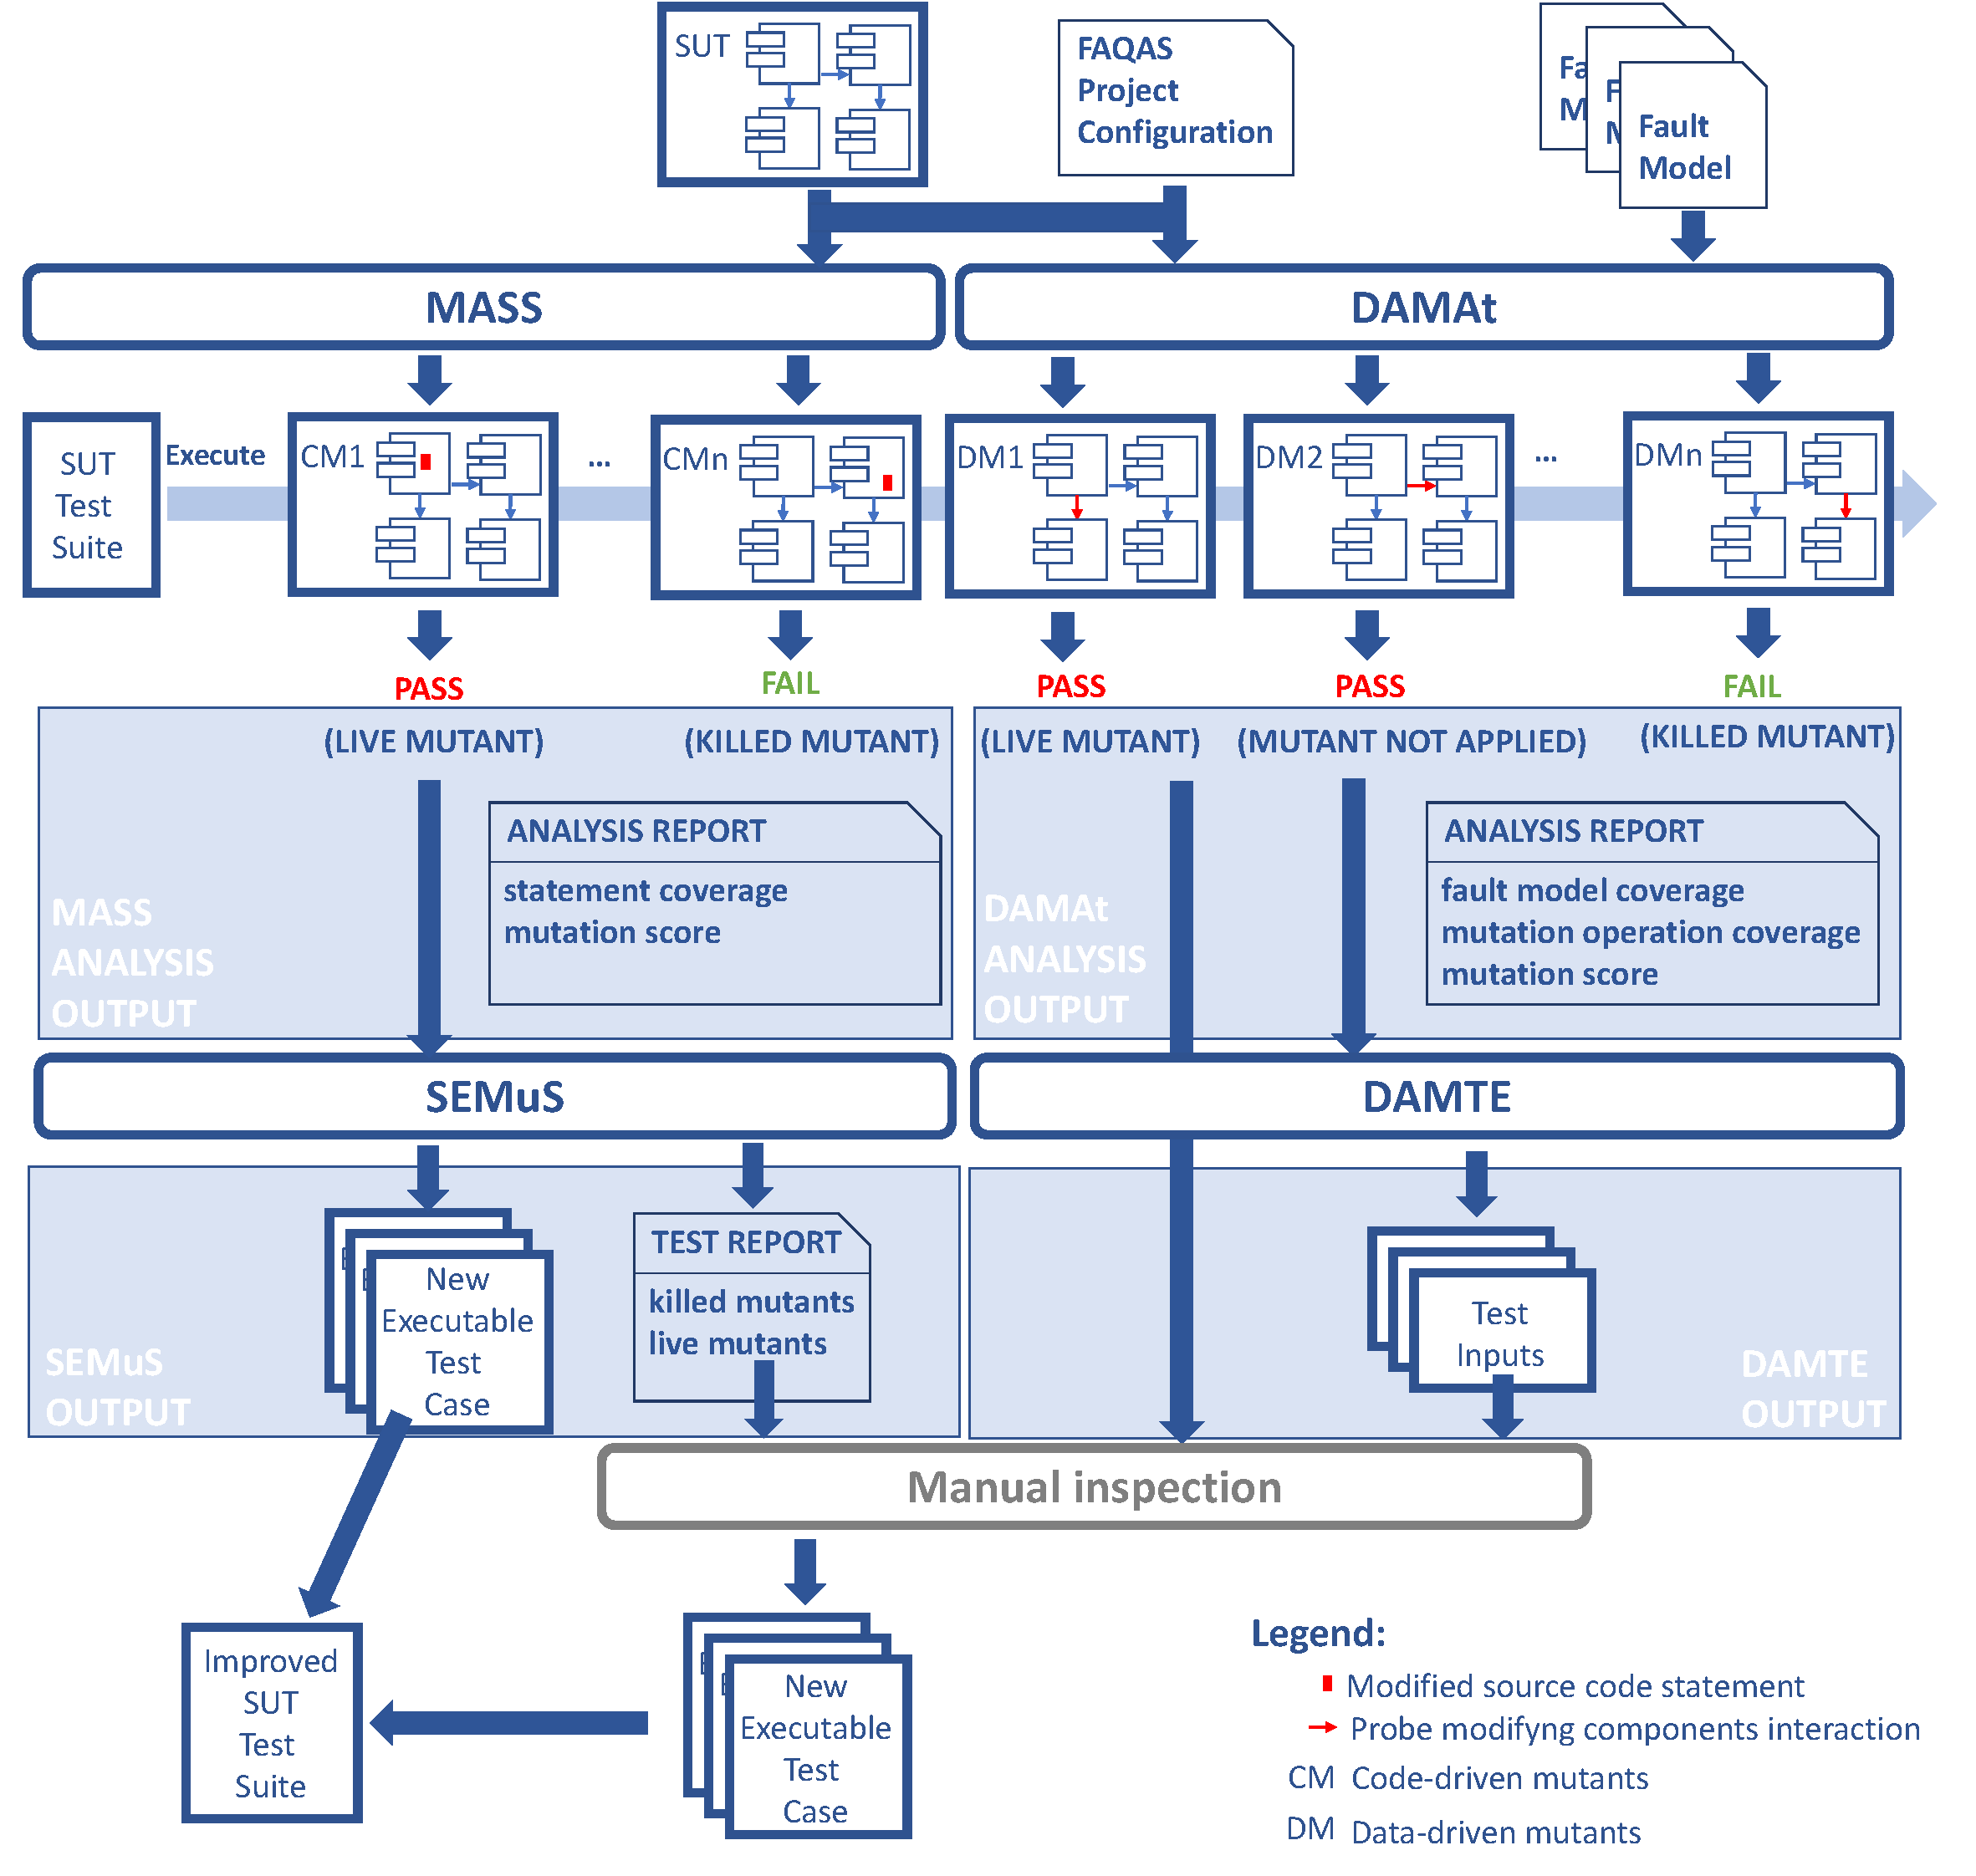
\includegraphics[width=0.7\textwidth]{images/FAQAS-overview.pdf}
\caption{Overview of the FAQAS toolset}
\label{fig:FAQAS:toolset}
\end{center}
\end{figure*}

Figure~\ref{fig:FAQAS:toolset} provides an overview of the input and outputs of the FAQAS toolset. It relies on the idea of generating multiple modified versions of the software system under test (SUT), some are derived by modifying the implementation of the software (code-driven mutants) other by integrating a mutation API that alters the messages exchanged by the software components of the SUT (data-driven mutants). 
The SUT test suite shall be executed with all the mutants, if it is effective then it shall fail with each of them. The mutants for which a failure is not observed are said to be \EMPH{live} and indicate a pitfall in the test suite.
All the FAQAS tools take as input the software under test (SUT), its test suite, and a set of configuration files. 

\EMPH{MASS} generates code-driven mutants. It integrates a pipeline of solutions that make mutation analysis feasible with large SUT. The three main contributions of MASS are (1) the automated identification of trivially equivalent mutants using an ensemble of compiler optimization options, (2) the computation of the mutation score based on mutant sampling with fixed size confidence interval approach (FSCI), (3) the automated identification of equivalent mutants based on coverage. 
MASS reports the set of live mutants, the set of killed mutants (i.e., mutants that are discovered by the test suite), and information useful to draft a verification report, which includes the statement coverage of the SUT test suite and the mutation score (i.e., the percentage of mutants discovered by the test suite).

\EMPH{DAMAt} generates mutants for data-driven mutation analysis. Data-driven mutation analysis is a research contribution of FAQAS. Instead of mutating the implementation of the SUT, it consists of altering the data exchanged by software components. 
DAMAt relies on fault models that specify how to mutate the data exchanged by software components through data-driven mutation operators. DAMAt can automatically alter data that is stored in data buffers (e.g., before serialization on the communication channel).
DAMAt enables the simulation of faults that affect simulated components (e.g., sensors), which is not feasible with traditional, code-driven mutation analysis. 
DAMAt generates as output a set of killed mutants (i.e., mutants that, during testing, successfully alter the data, and lead to test case failures), a set of live mutants (i.e., mutants that, during testing, successfully alter the data, but do not lead to test case failures), and a set of mutants not applied (i.e., mutants that, during testing, could not alter any data because the data they target is never exercised by the SUT); also, it provides information useful to draft a verification report, which includes the fault model coverage (i.e., percentage of fault models with at least one mutant applied), the mutation operation coverage (i.e., percentage of mutants applied), and the mutation score.

\EMPH{SEMuS} automatically generates executable unit test cases based on code-driven mutation analysis results. The generated unit test cases detect mutants not detected by the original test suite. The generated test cases include test oracles that shall be manually validated by engineers, which enables detecting faults. The generated test cases can be integrated into regression test suites.

SEMuS takes as input the list of live mutants detected by MASS. It generates a set of additional test cases that can be integrated into the SUT test suite. Also, it reports the list of killed mutants and the list of mutants that remain live (i.e., for which SEMuS did not generate a test case that kill them). Live mutants shall be manually inspected by engineers to either determine if they are equivalent or to manually derive a test case capable of killing them.

\EMPH{DAMTE} is a manual procedure supported by an automated symbolic execution toolset; it automatically identifies the test inputs that make software components exchange the data targeted by data-driven mutation operators. The derived test inputs can then be manually integrated into the SUT test suite.
 
The activity also included an extensive empirical evaluation demonstrating the feasibility, effectiveness, and scalability of the proposed toolsets in the space context, as described in the following sections.
 
%FAQAS.drawio.pdf

%Sections~\ref{ch:mass:approach} to~\ref{sec:data:test_suite_augmentation} provide an overview of the FAQAS tools: MASS, SEMuS, DAMAt, and DAMTE.
%Section~\ref{chapter:caseStudies} introduces the case study subjects considered for empirical evaluation.
%Section~\ref{sec:summary:results} provides an overview of the empirical results obtained.
%Section~\ref{sec:conclusion} concludes this report.



% !TEX root =  Main.tex
\section{Code-driven Mutation Analysis: MASS}
\label{ch:mass:approach}

\subsection{Overview}
\label{sec:approach}

\begin{figure}[tb]
\begin{center}
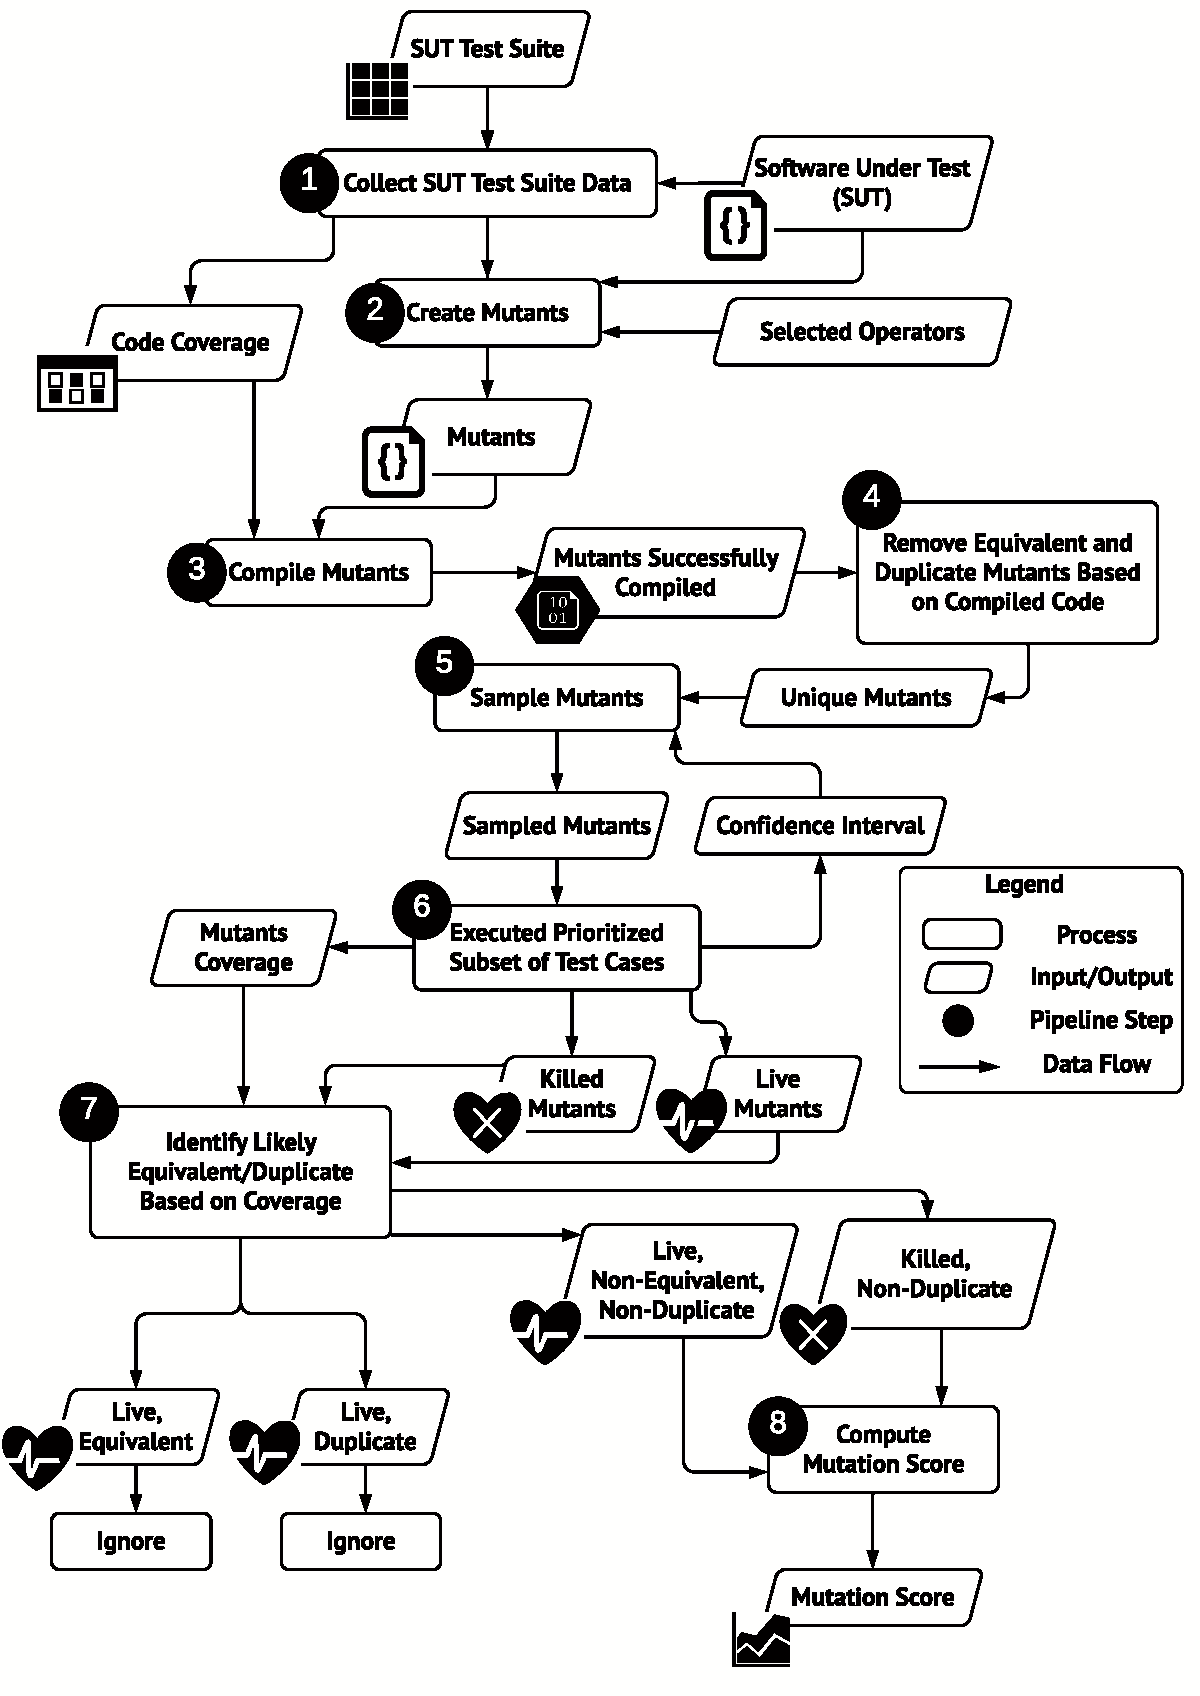
\includegraphics[width=0.6\textwidth]{images/Approach}
\caption{Overview of MASS}
\label{fig:approach}
\end{center}
\end{figure}

Figure~\ref{fig:approach} provides an overview of the mutation analysis process that we propose, \emph{Mutation Analysis for Space Software (\APPR)}. Its goal is to propose a comprehensive solution for making mutation analysis applicable to embedded software in industrial cyber-physical systems. \JMR{3.4}{The ultimate goal of \APPR is to assess the effectiveness of test suites with respect to detecting violations of functional requirements.}
 
\JMR{3.3}{Different from the mutation analysis pipeline presented in related work~\cite{papadakis2019mutation}, \APPR enables the integration of all mutation analysis optimization techniques that are feasible in our context to address scalability and pertinence problems (see Section~\ref{sec:back:summary}). 
\APPR consists of eight steps: (Step 1) Collect SUT Test Suite Data, (Step 2) Create Mutants, (Step 3) Compile Mutants, (Step 4) Remove Equivalent and Duplicate Mutants Based on Compiled Code, (Step 5) Sample Mutants,  (Step 6) Execute Prioritized Subset of Test Cases, 
(Step 7) Identify Likely Equivalent / Duplicate mutants Based on Coverage, and
(Step 8) Compute the Mutation Score. Different from related work, \APPR enables FSCI-based sampling by iterating between mutants sampling (Step 5) and test cases execution (Step 6). 
Also, it integrates test suite prioritization and reduction (Step 6) before the computation of the mutation score.
Finally, it includes methods to identify likely equivalent and duplicate mutants based on code coverage (Step 7).}
We describe each step in the following paragraphs. 

\clearpage
\subsection{Step 1: Collect SUT Test Data}

In Step 1, the test suite is executed against the SUT 
%software under test (SUT) 
and code coverage information is collected. 
More precisely, we rely on the combination of gcov~\cite{GCOV}
and GDB~\cite{GDB}, enabling the collection of coverage information for embedded systems without a file system~\cite{THANASSIS}.
% and Vector CAST~\cite{VectorCAST} 
%to record the number of times each line of code of the SUT has been exercised by a test case.

\subsection{Step 2: Create Mutants}

In Step 2, we automatically generate mutants for the SUT by relying on a set of selected mutation operators.
In \APPR, we rely on an extended sufficient set of mutation operators, which are listed in Table~\ref{table:operators}.
%In addition, in our experiments, we also evaluate the feasibility of relying only on the SDL operator, combined or not with OODL operators, instead of the entire sufficient set of operators.

% !TEX root =  ../Main.tex

\newcommand{\op}{\mathit{op}}
\newcommand{\ArithmeticSet}{ \texttt{+}, \texttt{-}, \texttt{*}, \texttt{/}, \texttt{\%} }
\newcommand{\LogicalSet}{ \texttt{&&}, \texttt{||} }
\newcommand{\RelationalSet}{ \texttt{>}, \texttt{>=}, \texttt{<}, \texttt{<=}, \texttt{==}, \texttt{!=} }
\newcommand{\BitWiseSet}{ \texttt{\&}, \texttt{|}, \land }
\newcommand{\ShiftSet}{ \texttt{>>}, \texttt{<<} }


\begin{table}[h]
\caption{Implemented set of mutation operators.}
\label{table:operators} 
\centering
\scriptsize
\begin{tabular}{|@{}p{4mm}@{}|@{}p{2cm}@{\hspace{1pt}}|@{}p{11.1cm}@{}|}
\hline
&\textbf{Operator} & \textbf{Description$^{*}$} \\
\hline
\multirow{7}{*}{\rotatebox{90}{\emph{Sufficient Set}}}&ABS               & $\{(v, -v)\}$	\\
\cline{2-3}
&AOR               & $\{(\op_1, op_2) \,|\, \op_1, \op_2 \in \{ \ArithmeticSet \} \land \op_1 \neq \op_2 \} $       \\
&    			  & $\{(\op_1, \op_2) \,|\, \op_1, \op_2 \in \{\texttt{+=}, \texttt{-=}, \texttt{*=}, \texttt{/=}, \texttt{\%} \texttt{=}\} \land \op_1 \neq \op_2 \} $       \\
\cline{2-3}
&ICR               & $\{i, x) \,|\, x \in \{1, -1, 0, i + 1, i - 1, -i\}\}$           \\
\cline{2-3}
&LCR               & $\{(\op_1, \op_2) \,|\, \op_1, \op_2 \in \{ \texttt{\&\&}, || \} \land \op_1 \neq \op_2 \}$            \\
&				  & $\{(\op_1, \op_2) \,|\, \op_1, \op_2 \in \{ \texttt{\&=}, \texttt{|=}, \texttt{\&=}\} \land \op_1 \neq \op_2 \}$            \\
&				  & $\{(\op_1, \op_2) \,|\, \op_1, \op_2 \in \{ \texttt{\&}, \texttt{|}, \texttt{\&\&}\} \land \op_1 \neq \op_2 \}$            \\
\cline{2-3}
&ROR               & $\{(\op_1, \op_2) \,|\, \op_1, \op_2 \in \{ \RelationalSet \}\}$            \\
&				  & $\{ (e, !(e)) \,|\, e \in \{\texttt{if(e)}, \texttt{while(e)}\} \}$ \\
\cline{2-3}
&SDL               & $\{(s, \texttt{remove}(s))\}$            \\
\cline{2-3}
&UOI               & $\{ (v, \texttt{--}v), (v, v\texttt{--}), (v, \texttt{++}v), (v, v\texttt{++}) \}$            \\   
\hline
\hline
\multirow{5}{*}{\rotatebox{90}{\emph{OODL}}}&AOD               & $\{((t_1\,op\,t_2), t_1), ((t_1\,op\,t_2), t_2) \,|\, op \in \{ \ArithmeticSet \} $       \\ 
\cline{2-3}
&LOD               & $\{((t_1\,op\,t_2), t_1), ((t_1\,op\,t_2), t_2) \,|\, op \in \{  \} \}$       \\ 
\cline{2-3}
&ROD               & $\{((t_1\,op\,t_2), t_1), ((t_1\,op\,t_2), t_2) \,|\, op \in \{ \RelationalSet \} \}$       \\ 
\cline{2-3}
&BOD               & $\{((t_1\,op\,t_2), t_1), ((t_1\,op\,t_2), t_2) \,|\, op \in \{ \BitWiseSet \} \}$       \\ 
\cline{2-3}
&SOD               & $\{((t_1\,op\,t_2), t_1), ((t_1\,op\,t_2), t_2) \,|\, op \in \{ \ShiftSet \} \}$       \\ 
%\hline
%COR               & $\{(\op_1, \op_2) \,|\, \op_1, \op_2 \in \{ \texttt{\&\&}, \texttt{||}, \land \} \land \op_1 \neq \op_2 \}$            \\
\hline
\hline
\multirow{3}{*}{\rotatebox{90}{\emph{Other}}}&LVR			& $\{(l_1, l_2) \,|\, (l_1, l_2) \in \{(0,-1), (l_1,-l_1), (l_1, 0), (\mathit{true}, \mathit{false}), (\mathit{false}, \mathit{true})\}\}$\\
&&\\
&&\\
\hline
\end{tabular}

$^{*}$Each pair in parenthesis shows how a program element is modified by the mutation operator. Th eleft element of the pair is replaced with the right element. We follow standard syntax~\cite{kintis2018effective}. Program elements are literals ($l$), integer literals ($i$), boolean expressions ($e$), operators ($\op$), statements ($s$), variables ($v$), and terms ( $t_i$, which might be either variables or literals).
\end{table}

%To automatically generate mutants, we have extended SRCIRor~\cite{hariri2018srciror} to include all the 
%operators in Table~\ref{table:operators}. 
%After mutating the original source file, our extension saves the mutated source file and keeps track of the mutation applied. Our toolset is available under the ESA Software Community Licence Permissive~\cite{ESAlicence} at the following URL \textbf{https://faqas.uni.lu/}.

\subsection{Step 3: Compile mutants}
\label{sec:appr:compile}

In Step 3, we 
compile mutants by relying on an optimized compilation procedure that leverages the build system of the SUT. To this end, we have developed a toolset that, for each mutated source file: (1) backs-up the original source file, (2) renames the mutated source file as the original source file, (3) runs the build system (e.g., executes the command \texttt{make}), (4) copies the generated executable mutant in a dedicated folder, (5) restores the original source file. Mutants that lead to compilation errors are discarded.

%Build systems \JMR{1.15}{(e.g., GNU make~\cite{MAKE} driving the GCC~\cite{GCC} compiler)} create one object file for each source file to be compiled and then link these object files together into the final executable. 
%\CHANGED{After the first build, in subsequent builds, 
%build systems
%%they 
%recompile only the modified files and link them to the rest.}
%For this reason, our optimized compilation procedure, which modifies at most two source files for each mutant (i.e., the mutated file and the file restored to eliminate the previous mutation), can reuse almost all the compiled object files in subsequent compilation runs, thus speeding up the compilation of multiple mutants. The experiments conducted with our subjects have shown that 
%%additional optimizations are not necessary to make the compilation of mutants feasible.
%\CHANGED{our optimization is sufficient to make the compilation of mutants feasible for large projects. Other state-of-the-art solutions introduce additional complexity (e.g., change the structure of the software under test~\cite{untch1993mutation}) that does not appear to be justified by scalability needs.}
 
% Concerning compilation warnings, we assume the build system of the SUT has been properly configured; more precisely, if the system should compile without warnings, the compiler is expected to be configured to treat warnings as errors otherwise mutants that lead to warning are retained.}

\subsection{Step 4: Remove equivalent and redundant mutants based on compiled code}

In Step 4, we rely on trivial compiler optimizations to identify and remove equivalent and redundant mutants. 
\REVNOV{C-P-15}{We compile the original software and every mutant multiple times once for each every available optimization option (i.e., \texttt{-O0}, \texttt{-O1}, \texttt{-O2}, \texttt{-O3}, \texttt{-Os}, \texttt{-Ofast} in GCC) or a subset of them.
After each execution of the compiler, we compute the SHA-512 hash summary of the generated executable.}To detect equivalent mutants, \APPR compares the hash summaries of the mutants with that of the original executable. To detect duplicate mutants but avoid combinatorial explosion, \APPR focuses its comparison of hash summaries on pairs of mutants belonging to the same source file (restricting the scope of the comparison is common practice~\cite{kintis2017detecting}).
Hash comparison allows us to (1) determine the presence of equivalent mutants (i.e., mutants having the same hash as the original executable), and (2) identify duplicate mutants (i.e., mutants with the same hash). %Mutants that are identified as being either equivalent and duplicate mutants are ignored in the following steps of \APPR. 
Equivalent and duplicate mutants are then discarded. 

%We compare hash summaries rather than executable files because it is much faster, an important consideration when dealing with a large number of mutants.
%The outcome of Step 4 is a set of \INDEX{unique mutants}, i.e., mutants with compiled code that differs from the original software and any other mutant.


\subsection{Step 5: Sample Mutants}
\label{sec:codeDriven:samplingStep}
\STARTCHANGEDNOV


In Step 5, \APPR samples the mutants to be executed to compute the mutation score. 
\JMR{1.8 3.3}{\APPR does not selectively generate mutants but samples them from the whole set of successfully compiled, nonequivalent, and nonduplicated mutants (result of Steps 2 to 4). This choice aims to avoid sampling bias which may result from the presence of such mutants; indeed, there is no guarantee that these mutants, if they were discarded after being sampled, would be uniformly distributed across program statements. Our choice does not affect the feasibility of \APPR since Steps 2 to 4 have negligible cost.}

Our pipeline supports different sampling strategies: \INDEX{proportional uniform sampling}, \INDEX{proportional method-based sampling},  \INDEX{uniform fixed-size sampling}, and \INDEX{uniform FSCI sampling}, which is an innovative contribution of the FAQAS actvity~\cite{Oscar:MASS:TSE}. 

%The strategies \INDEX{proportional uniform sampling} and \INDEX{proportional method-based sampling} were selected based on the results of Zhang et al.~\cite{zhang2013operator}, who compared eight strategies for sampling mutants. 
%The former was the best performing strategy and consists of sampling mutants evenly across all functions of the SUT, i.e., sampling $r\%$ mutants from each set of mutants generated inside the same function.
%The latter consists of randomly selecting $r\%$ mutants from the complete mutants set. This is included in our study because it is simpler to implement and showed to be equivalent to stratified sampling strategies, based on recent work~\cite{gopinath2015hard}.
%
%The \INDEX{uniform fixed-size sampling} strategy stems from the work of Gopinath et al.~\cite{gopinath2015hard} and consists of selecting a fixed number $N_M$ of mutants for the computation of the mutation score. Based their work, with 1,000 mutants, one can guarantee an accurate estimation of the mutation score.
%% In our empirical evaluation, we assess the accuracy obtained for $N_M$ values across the range [100;1000].}
%
%In this paper, we introduce the \INDEX{uniform FSCI sampling} strategy that determines the sample size dynamically, while exercising mutants, based on a fixed-width sequential confidence interval approach.
%With \INDEX{uniform FSCI sampling}, we introduce a cycle between Step 6 and Step 5, such that a new mutant is sampled only if deemed necessary.
%% of the mutation testing results collected so far. 
% More precisely, \APPR iteratively selects a random mutant from the set of unique mutants and exercises it using the SUT test suite. 
%% The result of each mutant execution (i.e., killed or live) is treated as a Bernoulli trial that is used to compute the confidence interval according to the FSCI method. 
%Based on related work, we assume that the mutation score computed with a sample of mutants follows a binomial distribution (see Section~\ref{sec:scalability}).
%For this reason, to compute the confidence interval for the FSCI analysis, we rely on the Clopper-Pearson method since it is reported to provide the best results (see Section~\ref{sec:scalability}).
%Mutation analysis (i.e., sampling and testing a mutant) stops when the confidence interval is below a given threshold $T_{\mathit{CI}}$ (we use $T_{\mathit{CI}}=0.10$ in our experiments). More formally, given a confidence interval 
%$[\mathit{L}_{S};\mathit{U}_{S}]$, with $\mathit{L}_{S}$ and $\mathit{U}_{S}$ indicating the lower and upper bound of the interval, mutation analysis stops when the following condition holds:
%\begin{equation}
%\label{eq:CI:T}
%(\mathit{U}_{S}-\mathit{L}_{S})<T_{\mathit{CI}}.
%\end{equation}
%
%Unfortunately, the assumption about the estimated mutation score following a binomial distribution may not hold when a subset of the test suite is executed for every mutant (which could happen in Step 6). Without going into the details behind the implementation of Step 6, which is described in Section~\ref{sec:step:prioritize}, 
%we can expect that a reduced test suite may not be able to kill all the mutants killed by the entire test suite, i.e., the estimated mutation score may be affected by negative bias. Consequently, over multiple runs, the mean of the estimated mutation score may not be close to the \INDEX{actual mutation score} (i.e., the mutation score computed with the entire test suite exercising all the mutants for the SUT)
% but may converge to a lower value. 
%To compute a correct confidence interval that includes the actual mutation score of the SUT, we thus need to take into account this negative bias.
%
%To study the effect of negative bias on the confidence interval, we address first the relation between the actual mutation score and the mutation score computed with the reduced test suite when the entire set of mutants for the SUT is executed. 
%A mutant killed by the entire test suite has a probability $P_{\mathit{KErr}}$ of not being killed by the reduced test suite.
%The probability $P_{\mathit{KErr}}$  can be estimated as the proportion of mutants (erroneously) not killed by the reduced test suite 
%\begin{equation}
%P_{\mathit{KErr}} = \frac{|E_R|}{|M|}
%\end{equation}
%with 
%$E_R$ being the subset of mutants that are killed by the entire test suite but not by the reduced test suite, and $M$ being the full set of mutants for the SUT.
%
%The mutation score for the reduced test suite ($\mathit{MS}_R$) can be computed as
%
%\begin{equation}
%\small
%\mathit{MS}_R=\frac{|K|-|E_R|}{|M|}=\frac{|K|}{|M|}-\frac{|E_R|}{|M|}=\mathit{MS}-\frac{|E_R|}{|M|}=\mathit{MS}-P_{\mathit{KErr}}
%\end{equation}
%
%where $K$ is the set of mutants killed by the whole test suite, $M$ is the set of all the mutants of the SUT,  and $\mathit{MS}$ is the actual mutation score. Consequently, the actual mutation score can be computed as 
%\begin{equation}
%\label{eq:MS}
%\mathit{MS}=\mathit{MS}_R+P_{\mathit{Err}_R}
%\end{equation}
%
%We now discuss the effect of a reduced test suite on the confidence interval for a mutation score estimated with mutants sampling. When mutants are sampled and tested with the entire test suite, the actual mutation score is expected to lie in the confidence interval $[\mathit{L}_{S};\mathit{U}_{S}]$. 
%\CHANGED{In the presence of a reduced test suite, we can still rely on the Clopper-Pearson method to compute the confidence interval $\mathit{CI}_R=[\mathit{L}_{R};\mathit{U}_{R}]$.
%However, }
%%in the presence of a reduced test suite,
%we have to take into account the probability of an error in the computation of the mutation score $\mathit{MS}_R$;  $\mathit{MS}_R$ can be lower than $\mathit{MS}$ and, based on Equation~\ref{eq:MS}, we expect the actual mutation score to lie in 
%%the interval.
%\JMR{NEW}{an interval that is shifted with respect to the interval for $\mathit{MS}_R$:}
%
%\begin{equation}
%\label{eq:CI}
%\mathit{CI}=[\mathit{L}_{R}+P_\mathit{KErr};\mathit{U}_{R}+P_{\mathit{KErr}}]
%\end{equation}
%
%We can only estimate  $P_{\mathit{KErr}}$ since computing it would require the execution of all the mutants with the complete test suite, thus undermining our objective of reducing test executions. 
%To do so, we can randomly select a subset $M_R$ of mutants, on which to execute the entire test suite and identify the mutants killed by the reduced test suite. %\footnote{In our implementation, we record the outcome of each test case of the whole suite and then simulate the execution of the reduced test suite, thus saving time.} 
%The size of the set $M_R$ should be lower than the number of mutants we expect FSCI sampling to return, 
%%(e.g., we use $M_R=100$ in our experiments\footnote{Though it would be possible to also estimate $P_{\mathit{KErr}}$ with FSCI, we leave it for future work.}), 
%otherwise sampling would not provide any cost reduction benefit.
%Since, for every mutant in $M_R$, we can determine if it is erroneously reported as not killed by the reduced test suite R,
%we can 
%%end up with a vector of boolean evaluations $E=e_1, ..., e_n$ where each evaluation $e_i$ is equal to \emph{true} if the $i^{th}$ mutant has been erroneously indicated as not killed by the reduced test suite.
%%This population of evaluations enable us to 
%estimate the probability $P_{\mathit{KErr}}$ as the percentage of such mutants.
%As for the case of the mutation score, 
%%these mutants tend to be positively  correlated\footnote{If a line of code contains a mutant that is not killed by the reduced test suite, it may contain another such mutant.} and, for this reason,
%we assume that the binomial distribution provides a conservative estimate of the variance for $P_{\mathit{KErr}}$. 
%
%We can estimate the confidence interval for $P_{\mathit{KErr}}$ using one of the methods for binomial distributions.
%We rely on the Wilson score method because it is known to perform well with small samples~\cite{Newcombe:Wilson:1998}. 
%The value of $P_{\mathit{KErr}}$ will thus lie within $\mathit{CI}_E=[\mathit{L}_{E};\mathit{U}_{E}]$,  with $\mathit{L}_{E}$ and $\mathit{U}_{E}$ indicating the lower and upper bounds of the interval.
%
%
%
%\NEWFSCI{Based on Equation~\ref{eq:CI}, 
%%to ensure that the actual mutation score lies in the computed confidence interval, we should assume the worst case, i.e., $P_{\mathit{KErr}}=\mathit{U}_{E}$.
%the confidence interval to be used with FSCI sampling in the presence of a reduced test suite should thus be }
%\begin{equation}
%\label{eq:CI:FSCI}
%\mathit{CI}=[\mathit{L}_{R}+\mathit{L}_{E};\mathit{U}_{R}+\mathit{U}_{E}]
%\end{equation}
%
%\JMRCHANGE{The estimated mutation score is the value lying in the middle of the interval.}
%
%\UPDATE{Since the width of the confidence interval CI (hereafter, $|CI|$) results from the sum of $|\mathit{CI}_R|$ and $|\mathit{CI}_E|$,
%%Also, from a practical perspective, \JMRCHANGE{the terms $+\mathit{L}_{E}$ and} $+\mathit{U}_{E}$ may augment the size of the interval returned by the Clopper-Pearson method; consequently, 
%mutation sampling with a reduced test suite may lead to the execution of a larger set of mutants.}
%
%\UPDATE{Based on Equations~\ref{eq:CI:T} and~\ref{eq:CI:FSCI}, $|\mathit{CI}_R| \le T_{\mathit{CI}} - |\mathit{CI}_E|$.
%Consequently, when $|\mathit{CI}_E|>T_{\mathit{CI}}$, the reduced test suite cannot lead to sufficiently accurate results. 
%Also, a large $|\mathit{CI}_E|$ may prevent the identification of accurate results with a feasible number of mutants. For example, Clopper-pearson may require up to 1568 samples for a confidence interval below 0.05~\cite{Goncalves2012}}. 
%%the interval is 3.5, you will need a $[\mathit{L}_{R};\mathit{U}_{R}]$ of 7.5, which may require XXXX samples in the worst case).
%%https://select-statistics.co.uk/calculators/sample-size-calculator-population-proportion/
%%Basic Business Statistics, Global Edition, 13th Edition
%\UPDATE{
%We shall thus identify a threshold ($T_{\mathit{CE}}$) for the confidence interval $|\mathit{CI}_E|$ that enables 
%%$|\mathit{CI}_R| \le (T_{\mathit{CI}} - |\mathit{CI}_E|)$ 
%accurate estimates 
%with a small sample size (e.g., in the worst case, with less than 1000 samples, the sample size for related work).
%For this reason, starting from a minimal number of samples to estimate $P_{\mathit{KErr}}$ (150 in our experiments), \APPR keeps estimating $P_{\mathit{KErr}}$ until it yields $|\mathit{CI}_E| \le T_{\mathit{CE}}$. 
%In our experiments we set $T_{\mathit{CE}} = 0.035$.
%To select $T_{\mathit{CE}}$, we have identified a reasonable minimal mutation score to be expected in space software (i.e., 65\%) and identified, based on confidence interval estimation methods with finite population correction factor~\cite{BasicBusinessStatistics}, 
%the minimal value for $|\mathit{CI}_E|$ that requires a number of samples below 850 (i.e., $1000-150$).
%%Indeed, for a binomial proportion with a probability of success above 65\% (the minimal mutation score), a confidence interval width of 0.065 (i.e., $0.1-0.035$) shall be achieved with a sample size of 821.}
%}
%
%When it is not possible to estimate $|\mathit{CI}_E| \le T_{\mathit{CE}}$ \UPDATE{or when the number of samples required to estimate $|\mathit{CI}_E| \le T_{\mathit{CE}}$ is sufficient to accurately estimate the mutation score,} the test suite can be prioritized but not reduced and the confidence interval is computed using the traditional Clopper-Pearson method, i.e., $[\mathit{L}_{S};\mathit{U}_{S}]$.
%
%
%\ENDCHANGEDNOV

\subsection{Step 6: Execute prioritized subset of test cases}
\label{sec:step:prioritize}

In Step 6, we execute a prioritized subset of test cases. 
We select only the test cases that satisfy 
the reachability condition (i.e., cover the mutated statement) and  execute them in sequence.
Similarly to the approach of Zhang et al. \cite{zhang2013faster}, we define the order of execution of test cases based on their estimated likelihood of killing a mutant.
\CHANGED{However, in our work, this likelihood is estimated differently since, as discussed above, the measurements they rely on are not applicable in the context of system-level testing and complex cyber-physical systems 
(see Section~\ref{sec:scalability}).} \CHANGEDNOV{In contrast, to minimize the impact of measurements on real-time constraints, we only collect code coverage information for a small part of the system.}
%However, we redefined the criteria for the prioritization and selection of test cases because of the inapplicability of the ones proposed by Zhang et al. (see Section~\ref{sec:scalability}).

%However, we notice that such optimization may not be sufficient when test suites are particularly large; indeed, prioritizing test cases may not be sufficient to reduce execution time. For example, live mutants may lead to the execution of a large number of test cases when almost all the test cases of the test suite exercise the mutated statement. 
\REVNOV{C-P-46}{We execute only covered statements assuming that the test suite is optimal with respect to code coverage. More precisely, we addume that if a statement is not covered there is a good reason for it (e.g., it depends on hardware). 
If a statement is not covered by the test suite, there is no chance that a mutant generated in the non-covered statement can be possibly detected by any test case. 
If the test suite does not reach the required coverage there is no reason to perform mutation testing, because is already known that the test suite is not good.}

%To reduce the number of test cases to be executed with a mutant, 
%we should first execute the ones that more likely satisfy the necessity condition. 
%This might be achieved by executing a test case that exercises the mutated statement with variable values not observed before. 
%Unfortunately, in our context, the size of the SUT and its real-time constraints prevent us from recording all the variable values processed during testing. 
%
%Therefore, we rely on code coverage to determine if two test case executions exercise the mutated statement with diverse variable values. Such coverage is collected by efficient procedures provided by compilers, thus having lower impact on execution performance than other types of dynamic analysis solutions (e.g., tracing variable values).
%% as a surrogate indicator of  variable values diversity.
%%diversity in values assigned to the variables used in a statement. 
%Since, because of control- and data-flow dependencies, a different set of input values may lead to differences in code coverage, 
%the latter helps determine if two or more test cases likely exercise a mutated statement with different variable values. %Indeed, a difference in the set of 
%%statements covered by two test cases depends on the values reaching some of the program statements, including the mutated one.
%%Indeed, a difference in the set of 
%%statements covered by two or more test cases that exercise a same mutated statement may depend on the values used in such statement. 
%%For example, the definition of a variable may lead to the execution of different branches when different values are assigned across distinct executions.
%To increase the likelihood that the observed differences in code coverage are due to the use of different variable values to exercise the mutated statement, we restrict the scope of code coverage analysis 
%to the functions belonging to the component (i.e., the source file) that contains the mutated statement.
%%However, two test case executions may also present coverage differences 
%%because of a diverse set of variable values used by statements other than the mutated one. 
%%For this reason, we restrict the scope of code coverage analysis 
%%to the functions belonging to a same component (i.e., a same source file).
%Indeed, such functions typically present several control- and data-flow dependencies, thus 
%augmenting the likelihood that a coverage difference is due to the execution of the mutated statement with a diverse set of values. Also, collecting code coverage for a small part of the system further reduces the impact of our analysis on system performance.
%
%%to the mutated function, its callers, and its callees.
%%to maximize the chances that a change in the behaviour of the software depends on the values used in a mutated statement, we determine that two executions likely exercise a mutated statement with diverse values by focussing on the coverage of 
%%the mutated function, its callers, and its callees.
%%A reduced scope is effective in determining behavioural differences based on the analysis of variable valuations~\cite{Pastore:VART:2014}.
%
%%Since related work focuses on either statement coverage or the frequency of execution of a statement, 
%Based on related work, we have identified two possible strategies to characterize test case executions based on code coverage:
%\begin{itemize}
%\item[S1] Compare the sets of source code statements that have been covered by test cases~\cite{grun2009impact}.
%%\item[C2] Identify the set of unique pairs $\langle\mathit{statement},\mathit{arity}\rangle$, where $\mathit{statement}$ is a unique identifier for the source code statement, and $\mathit{arity}$ is a symbol (i.e., $1$ or $*$) indicating if the statement has been covered one or more times.
%\item[S2] Compare the number of times each statement has been covered by test cases~\cite{schuler2013covering}.
%\end{itemize}
%
%
%To determine how dissimilar two test cases are and, consequently, how likely they exercise the mutated statement with different values, we rely on widely adopted distance metrics. 
%In the case of S1, we rely on the Jaccard and Ochiai index, which are two similarity indices for binary data and have successfully been used to compare program executions based on code coverage~\cite{Zou:Ochiai:2019,Keller:Jaccard:2017,Briand:2019}. 
%\REVNOV{C-P-18}{The Jaccard index is also known as \INDEX{intersection over union} 
%it measures similarity between sets, and is defined as the size of the intersection divided by the size of the union.
%The Jaccard distance measures dissimilarity between sample sets and results from subtracting the Jaccard coefficient from 1.
%The Ochiai index calculates cosine similarity with binary data, it is used in molecular biology and software engineering.}
%Given two test cases $T_A$ and $T_B$, the Jaccard  ($D_J$) and Ochiai ($D_O$) distances are computed as follows:
%
%$D_J(T_a,T_b)=1-\frac{|C_a \cap C_b|}{|C_a \cup C_b|}$ \hspace{2mm} $D_O(T_a,T_b)=1-\frac{|C_a \cap C_b|}{\sqrt{|C_a| * |C_b|}}$, 
%where $C_a$ and $C_b$ are the set of covered statements exercised by $T_a$ and $T_b$, respectively.
%
%In the case of S2, we compute the distance between two test cases by relying on the euclidean distance ($D_E$) and the cosine similarity distance ($D_C$), two popular distance metrics used in machine learning.
%\REVNOV{C-P-18}{Euclidean distance is the straight-line distance between two points in Euclidean space; precisely, the Euclidean distance between two points is the length of the line segment connecting them. In our context, the two vectors consist of the number of times the program statements had been exercised by a test. Cosine similarity measures similarity between two vectors of an inner product space. It results from the inner product of the same vectors normalized to both have length 1, which matches the the cosine of the angle between them. It is widely adopted to measure cohesion within clusters in data mining.}
%Given two vectors $V_A$ and $V_B$, whose elements capture the number of times a statement has been covered by test cases $T_A$ and $T_B$, the distances $D_E$ and $D_C$ can be computed as follows:
%
%$D_E=\sqrt{\sum_{i=1}^{n}(A_i-B_i)^2}$
%
%$D_C= 1-\frac{\sum_{i=1}^{n}A_i*B_i}{\sqrt{\sum_{i=1}^{n}{A_i}^2}*\sqrt{\sum_{i=1}^{n}{B_i}^2}}$,
%%Their main difference is that cosine similarity is used when the magnitude of the vectors should not matter.
%where $A_i$ and $B_i$ refer to the number of times the i-th statement had been covered by $T_A$ and $T_B$, respectively.
%
%Figure~\ref{alg:prioritize} shows the pseudocode of our algorithm for selecting and prioritizing test cases. It generates as output
%a prioritized test suite (\INDEX{PTS}).
%Based on the findings of Zhang et al. \cite{zhang2013faster}, we first select the test case that exercises the mutated statement the highest number of times (Line~\ref{alg:prioritize:first}) \CHANGED{ and add it to the prioritized test suite (Line~\ref{alg:prioritize:add}).}
%Then, in the next iterations, the test case selected is the one with the largest distance from the closest test case already selected (Lines~\ref{alg:prioritize:selectStart} to~\ref{alg:prioritize:selectEnd}). 
%When two or more test cases have the same distance, we select randomly among the test cases that exercise the mutated statement the most.
%%is most different than any other test case already included in the prioritized test suite.
%
%%Then, since we aim to maximize test cases diversity, the next selected test case should be the one that is most different than any other test case already included in the prioritized test suite.
%%For this reason, for each test case $n$ not selected yet (Line~\ref{alg:prioritize:notSel}), we identify the test case $t$ showing the most similar coverage (i.e., the one with the minimal distance $d$, Line~\ref{alg:prioritize:minD}). We then select the test case $n$ with the highest distance from its closest test case (Lines~\ref{alg:prioritize:selectStart} to~\ref{alg:prioritize:selectEnd}). 
%
%The algorithm iterates as long as it identifies a test case
%showing a difference in code coverage from the 
%%that exercises 
%%the program statements differently than 
%already selected test cases (Line~\ref{alg:prioritize:until}).
%
%Test cases are then executed in the selected order. During  execution, we collect code coverage information and identify killed and live mutants.
%
%
%% !TEX root =  ../Main.tex

\newcommand{\INDA}{10}
\newcommand{\INDB}{15}
\newcommand{\INDC}{5}

%\vspace{-3mm}
\begin{figure}[tb]

\begin{algorithmic}[1]

%\footnotesize
\scriptsize
\Require \emph{TS}, the test suite of the software under test
\Require \emph{Cov}, coverage information, for each test case
\Require \emph{ms}, the mutated statement
\Ensure \emph{PTS}, a list of test cases to be executed, sorted by priority
% (source inputs, follow-up inputs, output data).

\State $\mathit{TS}_m \gets$ subset of $\mathit{TS}$ that cover the mutated statement $\mathit{ms}$, based on \emph{Cov} \label{alg:prioritize:select}
\State $\mathit{PTS} \gets \mathit{new} \mathit{list}$ \textcolor{darkgray}{//this list is initially empty}
\State $\mathit{PTS} \gets$ based on \emph{Cov} select from $\mathit{TS_m}$ the test case $t$ that exercises $\mathit{ms}$ more times \label{alg:prioritize:first}
\State $\mathit{PTS} \gets \mathit{PTS} \cup t$ \textcolor{darkgray}{//include first the test case selected above}  \label{alg:prioritize:add}

\State \textbf{repeat} \label{alg:prioritize:repeat}
\State \hspace{\INDC mm} \textbf{for each} $n$ in the set ($\mathit{TS}_m$ - $\mathit{PTS}$) \textcolor{darkgray}{, which is the set of test cases not already added to $\mathit{PTS}$} \label{alg:prioritize:notSel}
\State \hspace{\INDA mm} \textbf{for each} $t$ in $\mathit{PTS}$
\State \hspace{\INDB mm} compute the distance between $t$ and $n$
\State \hspace{\INDA mm} identify $t_n$ i.e., the test case $t$ with the minimal $d$ \label{alg:prioritize:minD}
\State \hspace{\INDC mm} among all the $t_n$ identified, select the one with the highest distance $d$ \label{alg:prioritize:selectStart}
\State \hspace{\INDC mm} \textbf{if} $d > 0$ \textcolor{darkgray}{//there is at least a test case with a different coverage}
\State \hspace{\INDA mm} \textcolor{darkgray}{//note: $n$ is the test case in the set ($\mathit{TS}_m$ - $\mathit{PTS}$) closer to $t_n$}
\State \hspace{\INDA mm} $\mathit{PTS} \gets \mathit{PTS} \cup n$ \label{alg:prioritize:selectEnd}
\State \textbf{until} $d > 0$ \label{alg:prioritize:until}


\end{algorithmic}
\vspace{-3mm}
\caption{Algorithm for prioritizing test cases}
%\vspace{-0.2cm}
\label{alg:prioritize}
\end{figure}




\subsection{Step 7: Discard Mutants}
\label{sec:algostepSeven}


In this step, we identify likely nonequivalent and likely nonduplicate mutants by relying on code coverage information \CHANGED{collected in the previous step}.

Similarly to related work~\cite{schuler2013covering}, 
%since the size of a program may determine the degree of non-determinism in statement coverage, 
we identify nonequivalent and nonduplicate mutants based on a threshold.

In our case, consistently with previous steps of \APPR,
we compute normalized distances based on the distance metrics $D_J$, $D_O$, $D_E$, and $D_C$. A mutant is considered nonequivalent when the distance from the original program is above the threshold $T_E$, for at least one test case.
Similarly, a mutant is considered nonduplicate when the distance from every other mutant is above the threshold $T_D$, for at least one test case. For the identification of nonequivalent mutants, we consider live mutants only. To identify nonduplicate mutants, we consider both live and killed mutants; however, to avoid combinatorial explosion, we compare only mutants belonging to the same source file (indeed, mutants belonging to different files are unlikely to be redundant). 
Killed mutants that lead to the failure of different test cases are not duplicate, regardless of their distance.

Thresholds $T_E$ and $T_D$ should enable the identification of mutants that are guaranteed to be nonequivalent and nonduplicate. In particular, we are interested in the set of \emph{live, nonequivalent, nonduplicate mutants} (hereafter, $\mathit{LNEND}$) and the set of \emph{killed, nonduplicate mutants} (hereafter, $\mathit{KND}$). With such guarantees, the mutation score can be adopted as an adequacy criterion in safety certification processes. For example, certification agencies may require safety-critical software to reach a mutation score of 100\%, which is feasible in the presence of nonequivalent mutants. 
%This will enable the adoption of mutation score as an adequacy criterion, 

%\REVNOV{C-P-19}{Figure~\ref{alg:nonEquivalent:nonRedeundat} shows the algorithm for detecting nonequivalent and nonduplicate mutants.
%It first identify among the list of killed mutants all the non-duplicate ones (Line~\ref{alg:equivalent:KND}).
%Then it identifies the non-equivalent mutants among the list of live mutants (Line~\ref{alg:equivalent:LNE}).
%Finally, it further filters the list of non-equivalent mutants to keep only the ones that appear to be nonduplicate (Line~\ref{alg:equivalent:LNEND}).}
%
%% !TEX root =  ../Main.tex

\renewcommand{\INDA}{5}
\renewcommand{\INDB}{10}
\renewcommand{\INDC}{15}
\newcommand{\INDD}{20}
\newcommand{\INDE}{25}

\renewcommand{\Comment}[1]{\textcolor{darkgray}{\textit{//#1}}}

%\vspace{-3mm}
\begin{figure}[tb]

\begin{algorithmic}[1]

%\footnotesize
\scriptsize
\Require \emph{D}, the distance function to use to identify equivalent/duplicate mutants
\Require \emph{KM}, list of killed mutants
\Require \emph{LM}, list of live mutants
\Require $\mathit{Cov}_O$, coverage information for all the test cases, for the original program
\Require $\mathit{Cov}_M$, coverage information for all the executed test cases, for every mutant
\Require \emph{TS}, list of test cases
\Require \emph{TR}, test results, for all the executions
\Ensure \emph{KNR}, a list of killed, non-duplicate  mutants
\Ensure \emph{LNENR}, a list of live, non-equivalent, non-duplicate mutants
% (source inputs, follow-up inputs, output data).

%\State $\mathit{TS}_m \gets$ subset of $\mathit{TS}$ that cover the mutated statement $\mathit{ms}$, based on \emph{Cov} \label{alg:equivalent:select}
%\State $\mathit{PTS} \gets \mathit{new} \mathit{list}$ \textcolor{darkgray}{//this list is initially empty}
%\State $\mathit{PTS} \gets$ based on \emph{Cov} select from $\mathit{TS_m}$ the test case $t$ that exercises $\mathit{ms}$ more times \label{alg:equivalent:first}
\State $\mathit{KNR} \gets \mathit{identifyNonDuplicateMutants(} \mathit{KM}, \mathit{TS}, \mathit{TR}, \mathit{Cov}_M)$ \label{alg:equivalent:KNR}
\State $\mathit{LNE} \gets \mathit{identifyNonEquivalentMutants(} \mathit{LNR}, \mathit{TS}, \mathit{Cov}_M, \mathit{Cov}_O)$ \label{alg:equivalent:LNE}
\State $\mathit{LNENR} \gets \mathit{identifyDuplicateMutants(} \mathit{LNE}, \mathit{TS}, \mathit{Cov}_M)$ \label{alg:equivalent:LNENR}


\Procedure{identifyNonDuplicateMutants}{$\mathit{M},\mathit{TS},\mathit{TR},\mathit{Cov}_M$}\Comment{$M$ is a  list of mutants, $\mathit{TS}$, $\mathit{TR}$, and $\mathit{Cov}_M$ are defined above}
\State $\mathit{NR} \gets \mathit{empty} \mathit{set}$
\State $\mathit{k1} \gets $ extract and remove first element of M
\State $\mathit{NR} \gets \mathit{NR} \cup \mathit{k1}$
\While {$\mathit{M}$ not empty}
\State $\mathit{k2} \gets $ extract and remove first element of M
\For {mutant $k1$ in $\mathit{NR}$}
\State $\mathit{duplicate}=\mathit{TRUE}$
\For {test case $t$ in $\mathit{TS}$}
\If {$t$ has different result in $k1$ and $k2$ }
\State $\mathit{duplicate}=\mathit{FALSE}$
\State \textbf{break}
\Else
\State $\mathit{cov}_{k1t} \gets $ extract coverage information for test case $t$ executed with mutant $k1$
\State $\mathit{cov}_{\mathit{k2}t} \gets $ extract coverage information for test case $t$ executed with mutant $k2$
\If {$D(\mathit{cov}_{k1t},\mathit{cov}_{\mathit{k2}t}) > T_R$ }
\State $\mathit{duplicate}=\mathit{FALSE}$
\State \textbf{break}
\EndIf
\EndIf
\EndFor
\If {$\mathit{duplicate}==\mathit{FALSE}$}
\State \textbf{break} \Comment{No need to compare with all the mutants if we know that it is not duplicate}
\EndIf
\EndFor
\If {$\mathit{duplicate}==\mathit{FALSE}$}
\State $\mathit{NR} \gets \mathit{NR} \cup \mathit{k2}$
\EndIf
\EndWhile
\State \textbf{return} $\mathit{NR}$
\EndProcedure


\Procedure{identifyNonEquivalentMutants}{$\mathit{M},\mathit{TS},\mathit{Cov}_M,\mathit{Cov}_O$}\Comment{$M$ is a  list of mutants, $\mathit{TS}$, and $\mathit{Cov}_M$, and $\mathit{Cov}_O$ are defined above}
\State $\mathit{NE} \gets \mathit{empty} \mathit{set}$
\While {$\mathit{M}$ not empty}
\State $\mathit{m} \gets $ extract and remove first element of M

\For {test case $t$ in $\mathit{TS}$}
\State $\mathit{cov}_{m} \gets $ extract coverage information for test case $t$ executed with mutant $m$
\State $\mathit{cov}_{o} \gets $ extract coverage information for test case $t$ executed with original program

\If {$D(\mathit{cov}_{m},\mathit{cov}_{o}) > T_E$ }
\State $\mathit{equivalent}=\mathit{FALSE}$
\State \textbf{break}
\EndIf

\EndFor

\If {$\mathit{equivalent}==\mathit{FALSE}$}
\State $\mathit{NE} \gets \mathit{NE} \cup \mathit{m}$
\EndIf

\EndWhile

\State \textbf{return} $\mathit{NE}$
\EndProcedure



%
%
%\State \hspace{\INDA mm} \textbf{if} $\mathit{KM}$ not empty
%\State \hspace{\INDB mm} compute the distance between $t$ and $n$
%\State \hspace{\INDA mm} identify $t_n$ i.e., the test case $t$ with the minimal $d$ \label{alg:equivalent:minD}
%\State \hspace{\INDC mm} among all the $t_n$ identified, select the one with the highest distance $d$ \label{alg:equivalent:selectStart}
%\State \hspace{\INDC mm} \textbf{if} $d > 0$ \textcolor{darkgray}{//there is at least a test case with a different coverage}
%\State \hspace{\INDA mm} \textcolor{darkgray}{//note: $n$ is the test case in the set ($\mathit{TS}_m$ - $\mathit{PTS}$) closer to $t_n$}
%\State \hspace{\INDA mm} $\mathit{PTS} \gets \mathit{PTS} \cup n$ \label{alg:equivalent:selectEnd}
%\State \textbf{until} $d > 0$ \label{alg:equivalent:until}


\end{algorithmic}
\vspace{-3mm}
\caption{Algorithm for identifying non-equivalent and non-duplicate mutants}
%\vspace{-0.2cm}
\label{alg:nonEquivalent:nonRedeundat}
\end{figure}



\subsection{Step 8: Compute Mutation Score}
\label{sec:appr:score}


The \INDEX{mutation score} (MS) is computed as the percentage of killed nonduplicate mutants 
%(hereafter, \emph{KND}) 
over the number of nonequivalent, nonduplicate mutants identified in Step 7):

\begin{equation}
\label{equation:ms}
\mathit{MS} = \frac{|\mathit{KND}|}{|\mathit{LNEND}|+|\mathit{KND}|}
\end{equation}
%Similarly,
%
%obof at lest one test case with respect
%
%
%The code coverage difference between the mutant and the original program is represented by a \textit{threshold T\%}, a difference of code coverage over a certain T\% indicates that both versions are not equivalent.


% !TEX root =  MAIN.tex

\newpage

\section{Code-driven Mutation Testing: SEMuS}

\subsection{Overview}
\label{sec:semus}





To achieve \INDEX{test suite augmentation} (i.e., automatically generate test cases that kill mutants), in FAQAS, we have implemented an extension of SEMu that we call SEMu for Space Software (\INDEX{SEMuS}).

%Symbolic Execution-based Mutant analysis for Space software (FAQAS-SEMuS), is an extension of SEMu that implements test generation for space software. 

% \TODO{I've extended the following paragraph; please check}

In the FAQAS context, we cannot use SEMu as it is, since it requires mutants to be compiled with the \INDEX{LLVM compiler} in LLVM-IR format. As demonstrated with our preliminary evaluation of existing mutation analysis tools, any analysis requiring compilation into LLVM format is unlikely applicable to space software because of two reasons:  (1) our case studies rely on compiler pipelines (e.g., RTEMS) that include architecture-specific optimizations that are not supported by LLVM, and (2) there is no guarantee that the compiled objects produced by LLVM are equivalent to those produced by the original compiler (e.g., memory allocation). 

To overcome the limitations above and \EMPH{apply the test generation approach of SEMu in FAQAS} we have implemented three solutions. 
First, to avoid mutants to behave differently than the original software because of LLVM specificities (case 2 above), we rely on  MASS to identify killed and live mutants, and then compile only the live mutants into LLVM-IR format. 
Second, to increase the likelihood of successfully compiling the SUT with LLVM (case 1 above),  instead of compiling the whole software, we compile only the mutated function and its dependencies, which enables the generation of unit test cases and shall be sufficient to ensure the quality of the system under test in this context (e.g., unit test cases are normally used to ensure high code coverage). Third, to enable the generation of the meta-mutants, which is necessary to apply SEMu, we have extended MASS to (1) generate, for each source file of the SUT, both a meta-mutant processed by SEMu and the mutants processed by MASS, and (2) trace each mutant, after mutation analysis, to each mutant contained into the meta-mutant. 





% \TODO{Please add an example of a meta-mutant and single mutants generated by MASS; also, add an sentence above to refer to such listings}





Figure~\ref{fig:semus_architecture} shows the architecture of SEMuS and how it interacts with MASS. SEMuS consists of five components, which are \INDEX{Test Template Generator},  \INDEX{Pre-SEMu},  \INDEX{KLEE-SEMu},  \INDEX{KTest to Unit Test}, and \INDEX{LLVM}.
They are detailed in the following paragraphs.

\begin{figure}[h]
\begin{center}
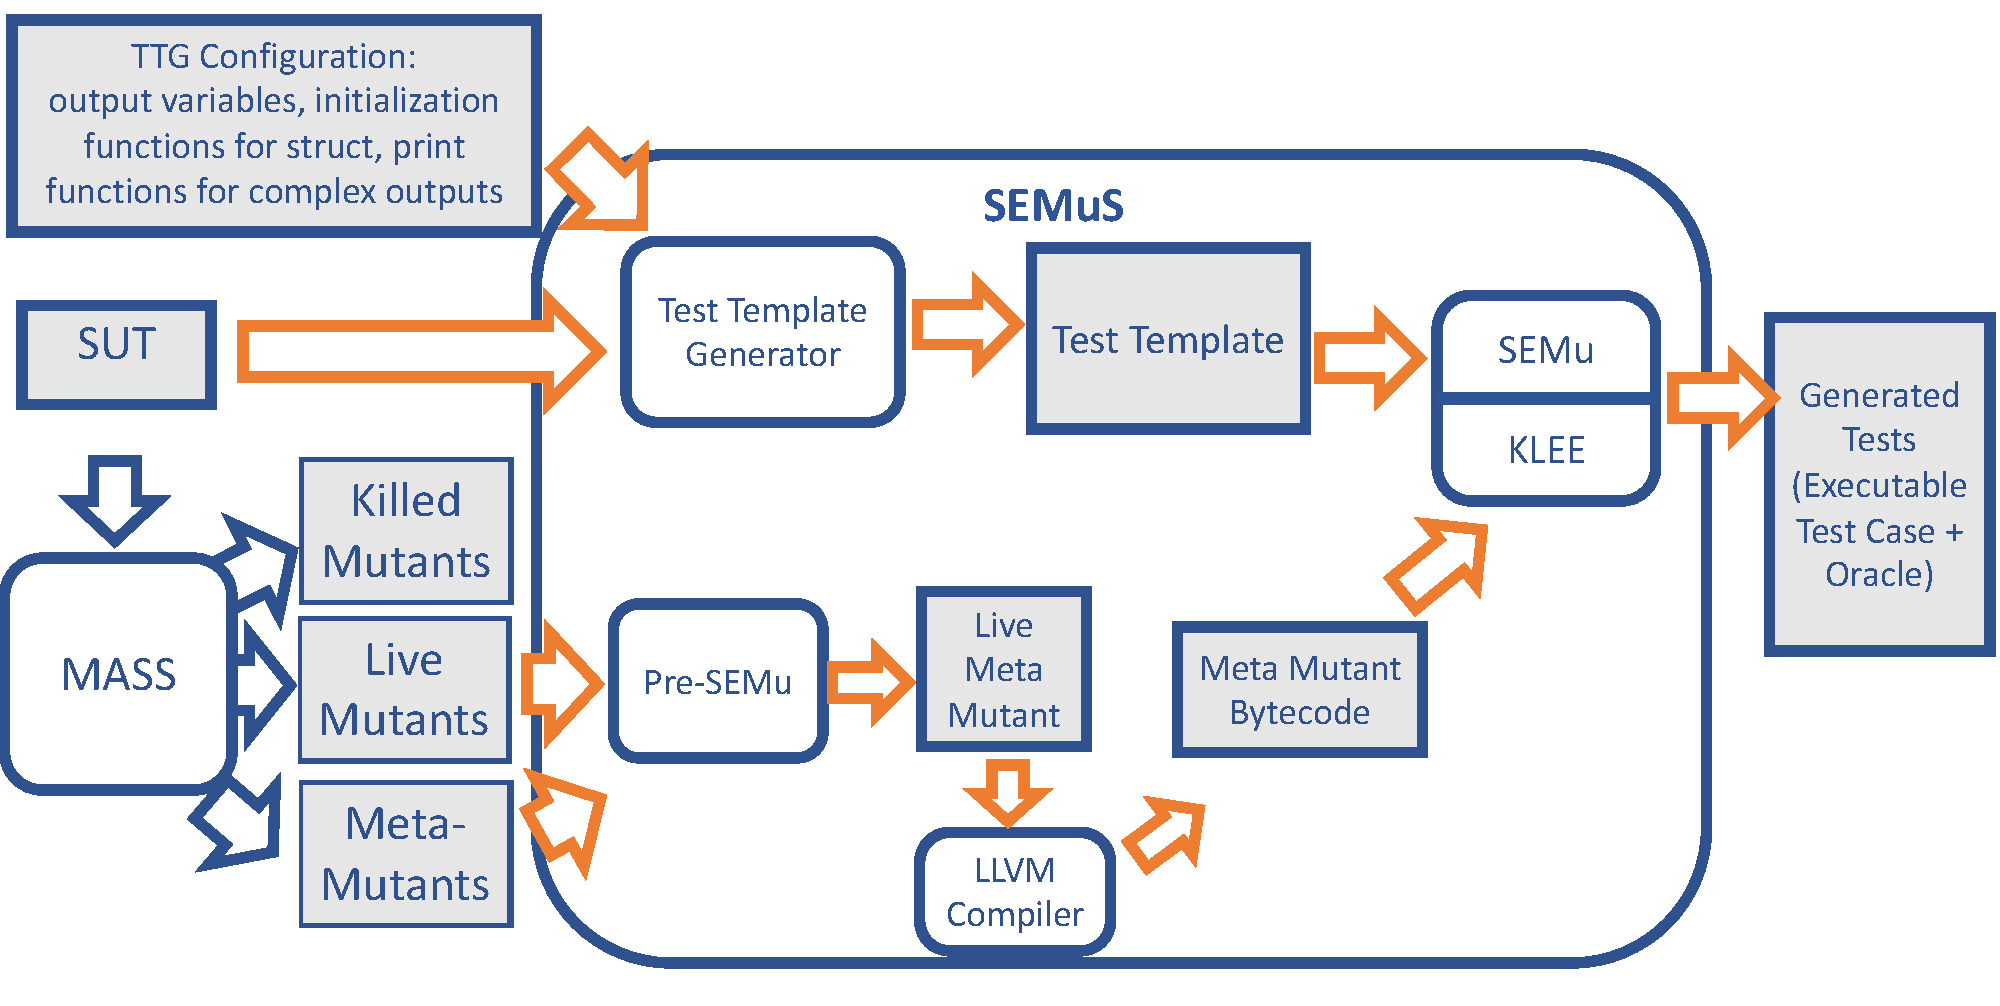
\includegraphics[width=0.8\textwidth]{images/semus-architecture2}
\caption{FAQAS-SEMuS Architecture and Workflow}
\label{fig:semus_architecture}
\end{center}
\end{figure}

%enable the adoption of SEMu in the space context. In particular, SEMuS (1) automates the generation of a test template including symbolic variables that guides the generation of test inputs, and (2) compiles the test template and the mutant into the format required by SEMu (i.e., LLVM-IR). 

\subsection{Test Template Generator}

The \INDEX{Test Template Generator} (TTG) component automates the generation of templates for the symbolic execution search. The component receives as inputs the SUT source code and the list of SUT functions. 

Listing~\ref{test_template} shows an example of a test template generated by the TTG. The TTG generates a template for every SUT function. The TTG parses the function arguments and declares them symbolic through use of the KLEE function \texttt{klee\_make\_symbolic}. Then, it adds a call to the function under analysis with symbolic values, and it saves the return value into a support variable (i.e., \texttt{result\_faqas\_semu} in Listing~\ref{test_template}). Finally, it generates a number of invocations of the \emph{printf} function that print the value of the software outputs and adds a return statement with the value returned by the function under test (e.g., \texttt{result\_faqas\_semu} in Listing~\ref{test_template}). 
Such \emph{printf} invocations are necessary because of the way SEMu determines that a mutant is killed; two are the cases in which the mutant is considered killed: (1) the main function returns a different return value, (2) different values are printed to the standard output. Consequently, it is necessary to print out all the values of the software outputs.
To select which variables to print, for every source file under test, the engineer can specify, in the SEMuS configuration file, the arguments (typically pointers) that should be either considered output or considered both input and outputs. By default, the TTG considers all the function arguments as inputs, in case some argument (e.g., a pointer to a memory buffer) is used both as input and as output the engineer shall specify it as such; similarly, in case some some argument (e.g., a pointer to a struct) is used to store outputs, the engineer shall indicate that it is an output. Moreover, since, in  the C language, the function \emph{printf} cannot automatically determine how to print the different fields specified in a data structure (i.e., it prints only the memory address of the pointer), the engineer can also specify how to printout the different fields of a data structure.

Listing~\ref{test_config} shows an example configuration file for SEMuS. In addition to output arguments (i.e., \emph{OUT\_\-ARGS\_NAMES}), input/output arguments (i.e., \emph{IN\_OUT\_ARGS\_NAMES}), and customized printf instructions (i.e., \emph{TYPES\_TO\_PRINTCODE}), the SEMuS configuration file enables the engineer to customize the generation of the test template further. Indeed, engineers can specify input argument types that should not be treated symbolically but that shall be initialized using a specific function of the SUT (i.e., \emph{TYPE\_TO\_INITIALIZATION\-CODE}); also, engineers can specify the fields, within such types (e.g., the attributes of a struct), that shall be treated symbolically.
Moreover, since the template returns the value of the function under test, the engineer can specify how to convert the returned value to int, if necessary (see parameter \emph{TYPES\_TO\_INTCONVERT}). Finally, in case the function under test receives a pointer to an array (which is typically passed as a pointer), the engineer can specify the size of such array (see parameter \emph{ARG\_TYPE\_TO\_ITS\_POINTER\_ELEM\_NUM}); by default, SEMuS assumes that a pointer refers to a single element (i.e., it is a pointer to a variable not an array).  


% !TEX root =  ../MAIN.tex

\begin{lstlisting}[style=CStyle, caption=SEMuS test template., label=test_template]
int main(int argc, char** argv) {
    // Declare variable to hold function returned value
    _Bool result_faqas_semu; 
    // Declare arguments and make input ones symbolic
    unsigned long pVal;
    int pErrCode;
    klee_make_symbolic(&pVal, sizeof(pVal), "pVal"); // Call function under test
    result_faqas_semu = T_INT_IsConstraintValid(&pVal, &pErrCode); // Make some output
    printf("FAQAS-SEMU-TEST_OUTPUT: %d\n", pErrCode);
    printf("FAQAS-SEMU-TEST_OUTPUT: %d\n", result_faqas_semu);
    return (int)result_faqas_semu;
}

\end{lstlisting}


\begin{lstlisting}[language={}, caption=Klee-test output, label=ktest]
ktest file : 'test000001.ktest'
args       : ['/MakeSym-TestGen-Input/direct/T_INT_IsConstraintValid/test.MetaMu.bc']
num objects: 2
object    0: name: b'model_version'
object    0: size: 4
object    0: data: b'\x01\x00\x00\x00'
object    1: name: b'pVal'
object    1: size: 8
object    1: data: b'\x00\x00\x00\x00\x00\x00\x00\x00'
\end{lstlisting}

% !TEX root =  ../MAIN.tex

\begin{lstlisting}[float=h, style=CStyle, caption=SEMuS configuration example., label=test_config]
{
"TYPES_TO_INTCONVERT": {},
"TYPES_TO_PRINTCODE": {"gs_timestamp_t": "printf(\"FAQAS-SEMU-TEST-OUTPUT: result_faqas_semu = tv_sec: %u, tv_nsec: %u\\n\", {}.tv_sec, {}.tv_nsec);"},
"OUT_ARGS_NAMES": ["pErrCode"],
"IN_OUT_ARGS_NAMES": ["base"],
"TYPE_TO_INITIALIZATIONCODE": {},
"TYPE_TO_SYMBOLIC_FIELDS_ACCESS": {},
"VOID_ARG_SUBSTITUTE_TYPE": "",
"ARG_TYPE_TO_ITS_POINTER_ELEM_NUM": {"char *": 6}
}
\end{lstlisting}


\subsection{Pre-SEMu}

The \INDEX{Pre-SEMu} component generates \INDEX{mutant schemata}; specifically, the component includes and compiles all the live mutants (i.e., MASS output) into a single bytecode file named the \emph{Meta Mutant}. SEMu will select which mutant to consider for test generation based on a parameter. The compilation of the Meta Mutant into LLVM bitcode is supported by the \emph{LLVM} compiler infrastructure. 

% !TEX root =  ../MAIN.tex



\begin{lstlisting}[style=CStyle, float=h, caption=Function T\_INT\_IsConstraintValid., label=original_meta]
flag T_INT_IsConstraintValid(const T_INT* pVal, int* pErrCode)
{
    flag ret = TRUE;
    (void)pVal;

    ret = ((*(pVal)) <= 50UL);
    *pErrCode = ret ? 0 :  ERR_T_INT;

    return ret;
}
\end{lstlisting}

\begin{lstlisting}[style=CStyle, float=h, caption=Mutant 1 of function T\_INT\_IsConstraintValid., label=meta_mutant_1]
flag T_INT_IsConstraintValid(const T_INT* pVal, int* pErrCode)
{
    flag ret = TRUE;
    (void)pVal;

    ret = ((*(pVal)) <= 50UL);
    *pErrCode = ret ? 1 :  ERR_T_INT;

    return ret;
}
\end{lstlisting}

\begin{lstlisting}[style=CStyle, float=h, caption=Mutant 2 of function T\_INT\_IsConstraintValid., label=meta_mutant_2]
flag T_INT_IsConstraintValid(const T_INT* pVal, int* pErrCode)
{
    flag ret = TRUE;
    (void)pVal;

    ret = ((*(pVal)) <= 50UL);
    *pErrCode = ret ? (-1) :  ERR_T_INT;

    return ret;
}
\end{lstlisting}

\begin{lstlisting}[style=CStyle, float=h, caption=Meta-Mutant for function T\_INT\_IsConstraintValid., label=meta_mutant_example]
flag T_INT_IsConstraintValid(const T_INT* pVal, int* pErrCode)
{
    flag ret = TRUE;
    (void)pVal;

    ret = ((*(pVal)) <= 50UL);

    klee_semu_GenMu_Mutant_ID_Selector_Func(1,2);
    *pErrCode = ret ? 
    	( klee_semu_GenMu_Mutant_ID_Selector==2 ?
    		((-1)):
		    (klee_semu_GenMu_Mutant_ID_Selector==1?
			    (1):
			    (0))) 
			    :  ERR_T_INT;
    klee_semu_GenMu_Post_Mutation_Point_Func(0,0);
    klee_semu_GenMu_Post_Mutation_Point_Func(1,2);

    return ret;
}
\end{lstlisting}

Listings~\ref{original_meta} provides the source code of function \emph{T\_INT\_IsConstraintValid}, while Listings~\ref{meta_mutant_1} and~\ref{meta_mutant_2} provide two example mutants generated by MASS.
Listing~\ref{meta_mutant_example} provides an example \INDEX{meta-mutant} including the same two mutants of Listings~\ref{meta_mutant_1} and~\ref{meta_mutant_2}. 
To select the mutants to analyze at runtime, SEMu relies on three support functions that shall be invoked within the eta-mutant:

\begin{itemize}
	\item \texttt{klee\_semu\_GenMu\_Mutant\_ID\_Selector\_Func}: function that takes two mutant IDs as arguments, representing a range of mutant IDs. It specifies where a portion of code containing mutants start.
    \item \texttt{klee\_semu\_GenMu\_Mutant\_ID\_Selector}: global variable that contains the ID of the mutant to be activated durng the analysis with SEMu.
	\item \texttt{klee\_semu\_GenMu\_Post\_Mutation\_Poin\_Func}: 
	function that takes two mutant IDs as arguments, it specifies where a portion of code containing mutants ends.
	It is used by SEMu to identify the portion of the code where to compare the state of the original and the mutated program and determine if the mutation has affected the program state (i.e., the \INDEX{necessity} condition to kill a mutant). In other words, it enables SEMu to perform conservative pruning and remove the mutant states that are not infected.
\end{itemize}

In Listing~\ref{meta_mutant_example}, mutant 2 from Listing~\ref{meta_mutant_2} appears on line 11 (indeed, the value \emph{-1} is selected when the mutant ID is equal to 2). Mutant 1 from Listing~\ref{meta_mutant_1} appears on line 12 (indeed, the value \emph{1} is selected when the mutant ID is equal to 1). The original software is represented by the mutant ID zero; indeed the value \emph{0} (i.e., what appears in line 7 of the Listing~\ref{original_meta}) is selected on line 14 (i.e., when the mutant ID is neither \emph{2} nor \emph{1}).

\subsection{KLEE-SEMu}



\INDEX{KLEE-SEMu} is the underlying test generation component, previously described in Section~\ref{sec:testGen:CP}. This component receives as inputs the \emph{LLVM bitcode} of the \emph{Meta Mutant} and the \emph{Test Template} for the function under test, and proceeds to apply dynamic symbolic execution to generate test inputs to kill the mutants. The output of this component are the \emph{KLEE tests}.

% \TODO{you need to list what are "the parameters of the execution"}
A \INDEX{KLEE test} is a binary file that contains information about the execution of KLEE such as the entry point of the analysis, and the generated test inputs.


An example of a KLEE test is presented in Listing~\ref{ktest}. The field \emph{args} report the entry point of the analysis; in this case, the test generation was performed for live mutants present in the function \texttt{T\_INT\_Is\-Constraint\-Valid}, which SEMuS stores in a dedicated folder. The fields named \emph{object} provide information about the outputs generated by KLEE (e.g., the generated test inputs). 
For each object, the KLEE test provides a \emph{name} (usually the name of the symbolic variable), its \emph{size}, and the actual \emph{value} generated by KLEE through constraint solving (usually this is reported in binary form).
Objects are numbered. Object number \emph{0} reports information about the data structure used by KLEE, that is, the version of the structure. The other objects report information about the generated test inputs.
Our example shows that one value of size 8 was generated for the variable \texttt{pVal}, the data field shows the binary representation of the \texttt{pVal} variable, in this case \texttt{pVal=0}.

% !TEX root =  ../MAIN.tex
\begin{lstlisting}[float=t, language={}, caption=Klee-test output, label=ktest]
ktest file : 'test000001.ktest'
args       : ['/MakeSym-TestGen-Input/direct/T_INT_IsConstraintValid/test.MetaMu.bc']
num objects: 2
object    0: name: b'model_version'
object    0: size: 4
object    0: data: b'\x01\x00\x00\x00'
object    1: name: b'pVal'
object    1: size: 8
object    1: data: b'\x00\x00\x00\x00\x00\x00\x00\x00'
\end{lstlisting}

\subsection{KTest to Unit Test}

% !TEX root =  ../MAIN.tex

\begin{lstlisting}[float=t, style=CStyle,  caption=Generated test case, label=gen_test_case]
#include <stdio.h>
#include <string.h>

#include "asn1crt.c"
#include "asn1crt_encoding.c"
#include "asn1crt_encoding_uper.c"


int main(int argc, char** argv)
{
    (void)argc;
    (void)argv;

    // Declare variable to hold function returned value
    _Bool result_faqas_semu;

    // Declare arguments and make input ones symbolic
    unsigned long pVal;
    int pErrCode;
    memset(&pVal, 0, sizeof(pVal));
    const unsigned char pVal_faqas_semu_test_data[] = {0x00, 0x00, 0x00, 0x00, 0x00, 0x00, 0x00, 0x00};
    memcpy(&pVal, pVal_faqas_semu_test_data, sizeof(pVal)); // Unsigned val is 0

    // Call function under test
    result_faqas_semu = T_INT_IsConstraintValid(&pVal, &pErrCode);

    // Make some output
    printf("FAQAS-SEMU-TEST_OUTPUT: pErrCode = %d\n", pErrCode);
    printf("FAQAS-SEMU-TEST_OUTPUT: result_faqas_semu = %d\n", result_faqas_semu);
    return (int)result_faqas_semu;
}
\end{lstlisting}



The component \INDEX{KTest to Unit Test} (KTU) converts a KLEE test into a human readable, compilable, and executable C test case. The unit test case generated by KTU, match the test template generated by TTG except for the declaration of variables where symbolic variables are replaced with concrete variables initialized with the values stored in the KTest file.
 
Listing~\ref{gen_test_case} shows an example of a test case generated for a mutant present in the function \texttt{T\_INT\_Is\-ConstraintValid}. For instance, line 20 shows that the variable \texttt{pVal} is initially filled with zeros, then in line 21, it is filled with the value stored in the variable \texttt{pVal\_faqas\_semu\_test\_data}, which holds the binary output produced by KLEE. In line 25, the function under test is invoked with the concrete value of \texttt{pVal}. 

The test case generated by the KTU prints the function return value and the value of every variable passed by reference, using the same instructions of the test template.
KTU cannot generate test assertions because only engineers can know, based on specifications, what are the values to be expected at the end of the test case execution.
However, the generated printf invocations still play the role of an oracle for regression testing, as explained in the next sections.

\subsection{Test suite augmentation} 
\label{sec:Semus:augment}
The procedure for testing with SEMuS is shown in Figure~\ref{fig:semus:test:example}.
In Step 1, the engineer executes SEMuS, which generates an output folder for every live mutant that is killed by the generated test cases.
Every folder contains: a script (i.e., \emph{runTest.sh}) that can be used to execute the generated test case, (2) the test case itself (i.e., test1.c), and (3) a text file with extension \emph{.expected} that contains the output that is observed when executing the test case with the SUT.
In Step 2, the engineer visually inspects every file with extension \emph{.expected} to determine if the observed output matches the specifications; if not, the software is faulty and needs to be fixed. In this case mutation testing enables detecting a fault. 
After verifying all the generated files with extension \emph{.expected} the engineer can reuse the test cases generated by SEMuS for regression testing in future versions of the SUT. Basically, the output folders generated by SEMuS become part of the test suite of the SUT.

When there is a new version of the SUT (Step 3, in Figure~\ref{fig:semus:test:example}), the folder with the source code of the SUT is replaced with the new version of the SUT (this can be done automatically with version control software).
The engineer can then trigger test execution by simply re-executing all the scripts \emph{runTest.sh} generated by SEMuS.
The script \emph{runTest.sh} first executes the test case (Step 4.1), then it stores the test outputs into a text file with extension \emph{.got}, finally if compares the observed output with the output generated for the previous version. If the function under test was not modified, differences may indicate that the test case FAILED.

\begin{figure}[h]
\begin{center}
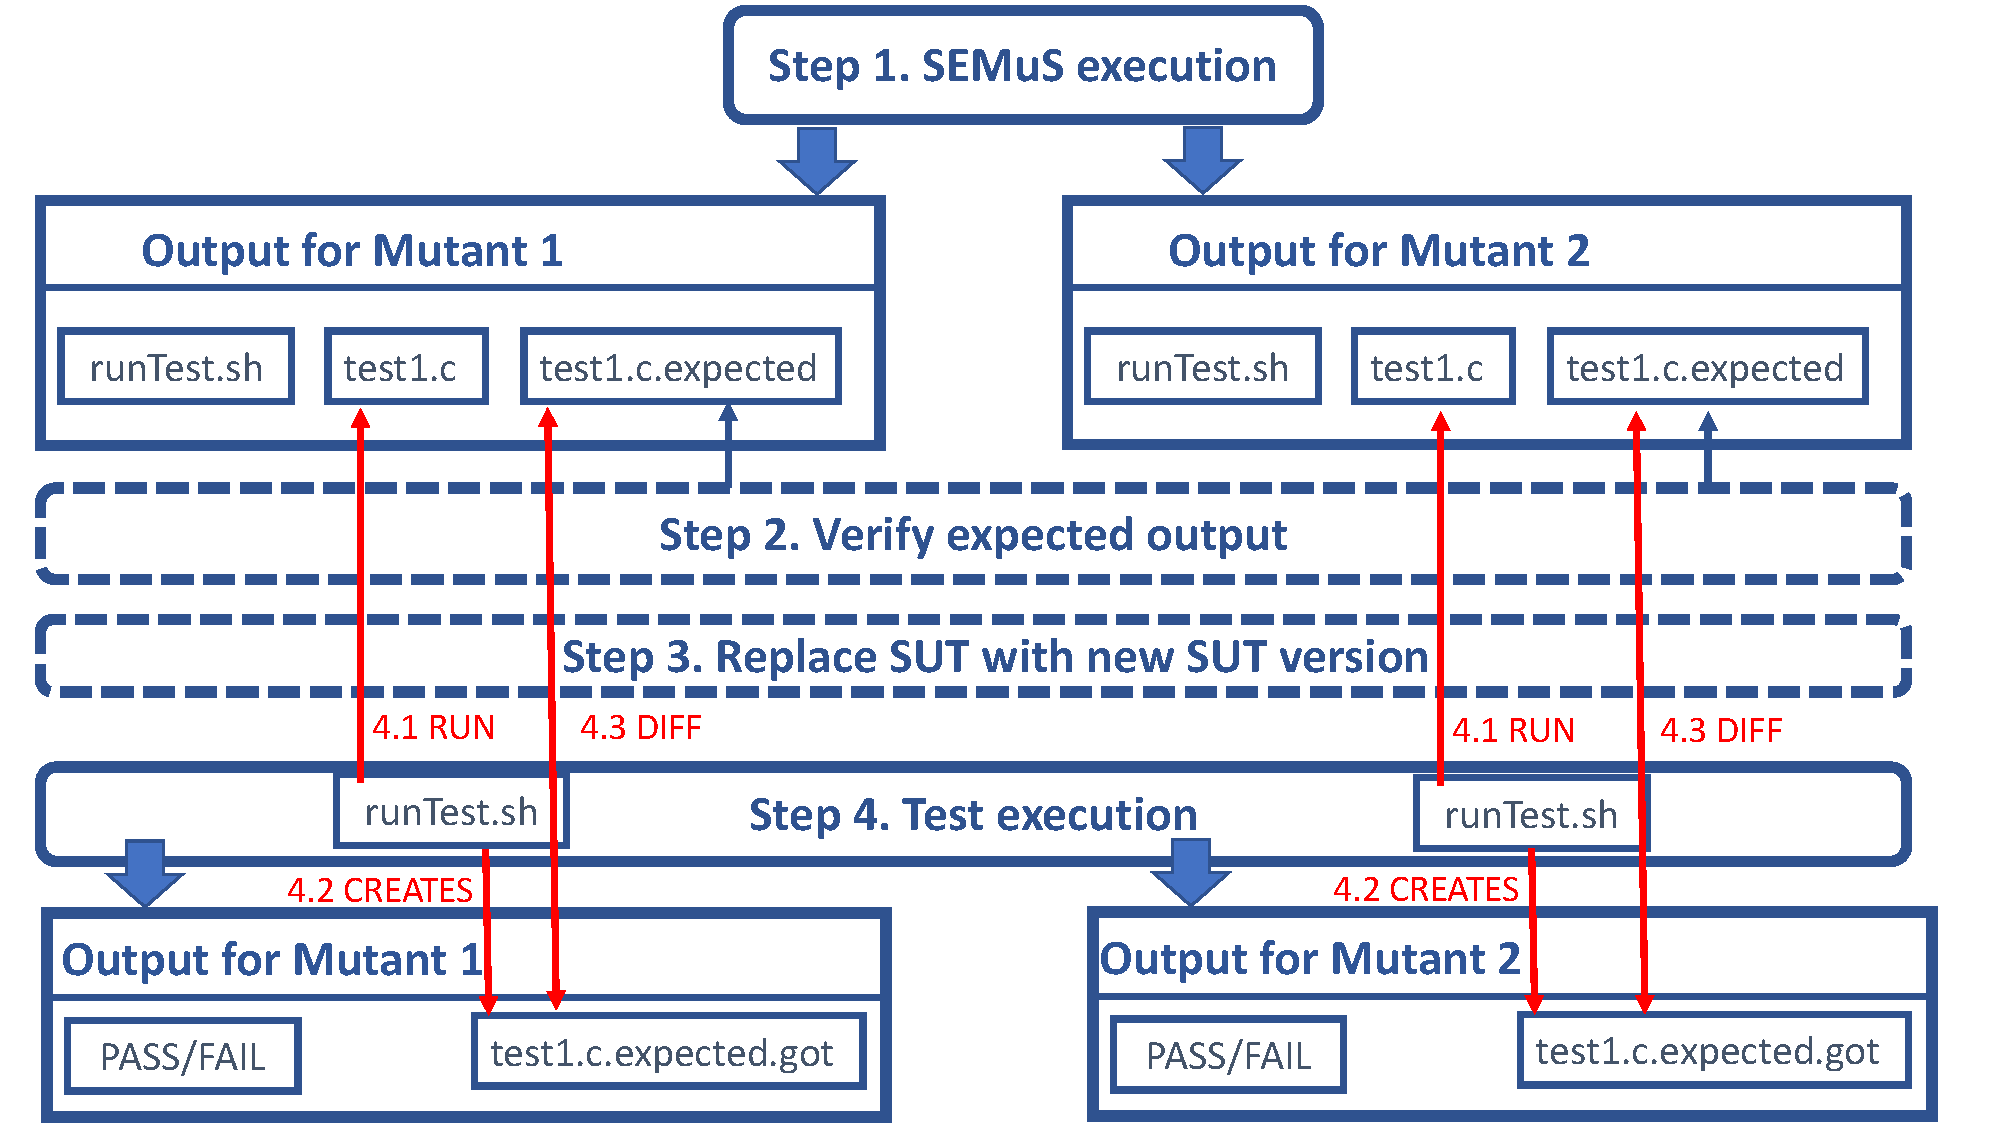
\includegraphics[width=0.8\textwidth]{images/semus-out}
\caption{Workflow for test suite augmentation with SEMuS}
\label{fig:semus:test:example}
\end{center}
\end{figure}

\subsection{Live mutants}

SEMuS may not be capable of selecting test inputs that kill the mutant under analysis. We may distinguish two cases:
\begin{itemize}
\item SEMuS execution terminates and no test case is generated.
\item SEMuS execution does terminate (i.e., it is killed after a timeout configured by the end-user, usually 15 minutes are sufficient to generate test cases).
\end{itemize}

In the first case, SEMuS has successfully exercised all the execution paths covering the mutated statements but did not identify inputs that satisfy the killing conditions. This may case indicate that the mutant is equivalent and may be discarded (however, the engineer shall verify that the test template is configured correctly). Also, we may be in such situations when some of the functions under test belong to libraries not compiled with LLVM that, consequently are not correctly processed by KLEE-SEMu; to detect these cases the engineer shall look for errors in the output generated by KLEE.

In the second case, SEMuS did not complete the analysis of the possible execution paths covering the mutated statement. Such cases may indicate that test generation is complex and probably an engineer may more efficiently select test inputs than the underlying constraint solving solution implemented by KLEE-SEMu.

% !TEX root =  ../MAIN.tex
\clearpage
\section{Data-driven Mutation Analysis: DAMAt}

\renewcommand{\APPR}{DAMAt\xspace{} }


\subsection{Overview}

In this Section, we propose \INDEX{data-driven mutation analysis}, 
a new mutation analysis paradigm
that alters the data exchanged by software components to evaluate the capability of a test suite to detect interoperability faults. Also, we present a technique, \INDEX{data-driven mutation analysis with tables} (\APPR),
to automate data-driven mutation analysis by relying on
a fault model that captures, for a specific set of components, both the characteristics of the data to mutate (e.g., the size and structure of the messages generated by the ADCS) and the types of fault that may affect such data (e.g., a  value out of the nominal range). The latter is formalized as a set of parameterizable mutation operators. 
To simplify adoption, we rely on fault models in tabular form where each row specifies, for a given data item, what mutation operator (along with its corresponding parameter values) to apply to which elements of the data item.
At runtime, \APPR modifies the data exchanged by components according to the provided fault model (e.g., replaces a nominal voltage value with a value out of the nominal range).






\INDEX{Data-driven mutation analysis} aims to evaluate the effectiveness of a test suite in detecting \INDEX{semantic interoperability \UPDATED{faults}}. 
It is achieved by modifying (i.e., mutating) the data exchanged by CPS components. It generates \INDEX{mutated data} that is representative of data that might be observed at runtime in the presence of a component that behaves differently than expected in the test case; also, it mutates  data that is not automatically corrected by the software 
(e.g., through cyclic redundancy check codes)
%(e.g., through CRC mechanisms, which aim to correct technical interoperability problems) 
and thus causes software failures (i.e., the mutated data shall have a different semantic than the original data). For these reasons, data mutation is driven by a fault model specified by the engineers based on domain knowledge.

Although different types of fault models might be envisioned,
%see background
we propose a technique (\INDEX{data-driven mutation analysis with tables}, \APPR),
which automates data-driven mutation analysis by relying on
a tabular \CHANGED{block model}, itself tailored to the \UPDATED{SUT} through predefined mutation operators.
To concretely perform data mutation at runtime, \APPR relies on a set of \INDEX{mutation probes} that shall be integrated by software engineers into the software layer that handles the communication between components. The runtime behaviour of mutation probes (i.e, what data shall be mutated and how) is driven by the fault model. Thus, \APPR can automatically generate the implementation of mutation probes from the provided fault model.
Depending on the CPS, probes might be inserted either into the \UPDATED{SUT}, into the simulator infrastructure, or both.
For example, Figure~\ref{fig:appr:mutateProbesInserted} shows the architecture of the \ESAIL satellite system with mutation probes integrated into the SVF
%\footnote{Software Validation Facility~\cite{Isasi2019}; it usually includes one or more simulators, an emulator to run the code compiled for the target hardware, and test harnesses.} 
functions that handle communication with external components (PDHU, GPS, and ADCS in this case). 






\APPR works in six steps, which are shown in Figure~\ref{fig:appr:approach}. 
In Step 1, based on the provided methodology and predefined mutation operators, the engineer prepares a fault model specification tailored to the SUT.
% capturing the data format and the types of faults that shall be injected for every data item exchanged by the system components.
In Step 2, \APPR generates a mutation API with the functions that modify the data according to the provided fault model.
In Step 3, the engineer modifies the \UPDATED{SUT} by introducing mutation probes (i.e., invocations to the mutation API) into it.
\REVTOOL{P-2}{Instead of modifying the SUT the engineer may modify the test harness (e.g., the SVF simulator); such choice depends on the software under test, if the test cases are executed through a simulator, such choice prevents introducing damaging changes into the SUT (e.g., delay task execution and break strict real-time requirements).}
In Step 4, \APPR generates and compiles mutants. 
Since the \APPR mutation operators may generate mutated data by applying multiple mutation procedures, \APPR may generate several mutants, one for each \UPDATED{mutation operation (i.e., a mutation procedure configured for a data item, according to our terminology, see Section~\ref{sec:mutantsGeneration})}.
In Step 5, \APPR executes the test suite with all the mutants including a mutant (i.e., the coverage mutant) which does not  modify the data but traces the coverage of the fault model.
In Step 6, \APPR generates mutation analysis results.

%\UPDATED{
%In our context, the \emph{software under test (SUT)} is the CPS embedded software that is verified by a test suite, which is the target of data-driven mutation analysis. Therefore, we refer to the software developed by the engineers as the \emph{original SUT}. An \emph{SUT mutant} (simply, a \emph{mutant}) is a version of the SUT that integrates a \emph{mutation probe} and shall make test cases fail. 
%%A mutation operator simulates one specific interoperability error (a specific type of that automatically alters data by applying one specific \emph{mutation operation}.
%}

In the following sections we describe the structure of our fault model and each step of \APPR.

\begin{figure}[h]
	\centering
		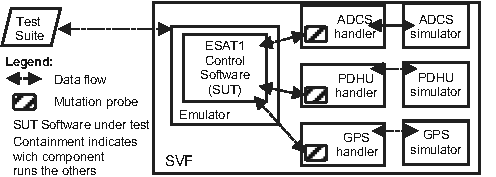
\includegraphics[width=8.4cm]{damat/images/dataMutationExample}
		\caption{\CHANGED{Data mutation probes integrated into \ESAIL.}}
		\label{fig:appr:mutateProbesInserted}
	\end{figure}

\begin{figure}[h]
	\centering
		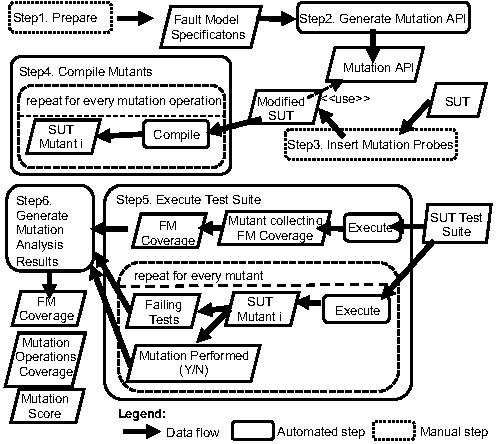
\includegraphics[width=8cm]{damat/images/dataDrivenBufferProcess}
		\caption{The \APPR process.}
		\label{fig:appr:approach}
	\end{figure}


\subsubsection{Fault Model Structure}
\label{sec:faultModelStructure}





The \APPR fault model enables the specification of the format of the data exchanged between components along with the type of faults that may affect such data. 
In this paper, we refer to the data exchanged by two components as \INDEX{message}; also, each CPS component may generate or receive different \INDEX{message types}.
For a single CPS, more than one fault model can be specified. For example, in the case of \ESAIL{} we have defined one fault model for every message type that could be exchanged by the three components under test (i.e., ADCS, PDHU, and GPS). In total, for \ESAIL, we have 14 fault models, 10 for the communication concerning ADCS (we have 10 different message types), 3 for PDHU, and 1 for GPS.

The \APPR fault model enables the modelling of data that is exchanged through a specific data structure: the data buffer. This was decided because it is a simple and widely adopted data structure for data exchanges between components in CPS. Also, more complex data structures (e.g., hierarchical ones like trees) are often flattened into data buffers in order to be exchanged by different components (e.g., through the network). When the CPS software is implemented in C or C++ (common CPS development languages) data buffers are implemented as arrays. Figure~\ref{fig:appr:bufferStructure} shows three block diagrams representing (part of) the buffer structure used to exchange messages of type InterfaceHouseKeeping and InterfaceStatus in \ESAIL.

A data buffer is characterized by a \INDEX{unit size} that specifies the dimension, in bytes, of the single cell of the underlying array and a \INDEX{buffer size}, which specifies the total number of units belonging to the buffer. Each data buffer can contain one or more \INDEX{data items}; the size of data items may vary as they may span over multiple units. Also, each data item is interpreted by the CPS software according to a specific \INDEX{representation} (e.g., integer, double, etc.). 
In \ESAIL, the unit size is one byte and the data items may span over one or two buffer units (see Figure~\ref{fig:appr:bufferStructure}). 
%Figure~\ref{} provides an example buffer instance for a \emph{Magnetorquer Set PWM RSP message}.

The \APPR fault model enables engineers to specify (1) the \emph{position} of each data item in the buffer, (2) their \emph{span}, and (3) their \emph{representation type}. Our current implementation supports six data representation types: int, long int, float, double, bin (i.e., data that should be treated in its binary form), hex (i.e., data that should be treated as hexadecimal).
Further, for each data item, \APPR enables engineers to specify one or more data faults using the mutation operator identifiers. For each operator, the engineer 
shall provide values for the required configuration parameters.

Table~\ref{table:operators} provides the list of mutation operators included in \APPR along with their description. The \APPR mutation operators generate \INDEX{mutated data item instances} through one or more \INDEX{mutation procedures}, which are the functions that generate a mutated data item instance given a correct data item instance observed at runtime. For example, the \emph{VAT} operator includes only one mutation procedure (i.e., setting the current value above the threshold) while the \emph{VOR} operator includes two mutation procedures, which are
(1) replacing the current value with a value above the specified valid range and (2) replacing the current value with a value below the valid range.
The operators VOR, BF, INV, and SS have been inspired by related work~\cite{di2015generating,PeachFuzzer,Matinnejad19}; the operators VAT, VBT, FVAT, FVBT, FVOR, IV, ASA,  and HV
are a contribution of this paper and were derived and conceptualised as a result of discussion with domain experts.
Although other data representation types (e.g., null terminated strings) and operators (e.g., replacement of a random char in a string) might be envisioned, in this paper, we focus on operators that are necessary in the CPS context, based on our experience.
For example, CPS components are unlikely to exchange strings.
%are a contribution of this paper, based on discussion with domain experts. 

\begin{figure}
	\centering
		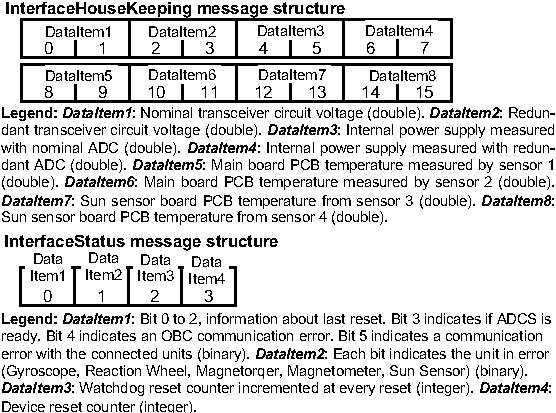
\includegraphics[width=8.4cm]{damat/images/BufferStructuresSmall}
		\caption{Structure of data buffers in \ESAIL.}
		\label{fig:appr:bufferStructure}
	\end{figure}
	
	% !TEX root = ../MAIN-DataDrivenMutationAnalysis.tex


\begin{table*}[tb]
\caption{Data-driven mutation operators}
\label{table:operators}
\scriptsize
\begin{tabular}{|p{40mm}|p{90mm}|}
\hline
\textbf{Fault Class}&\textbf{Description}\\
\hline
Value above threshold (VAT)&
Replaces the current value with a value above the threshold T for a delta (\D). 
\\
\hline
Value below threshold (VBT)&
Replaces the current value with a value below the threshold T for a delta (\D). 
\\
\hline
Value out of range (VOR)&
Replaces the current value with a value out of the range $[MIN;MAX]$.\\
\hline
Bit flip (BF)&
A number of bits randomly chosen in the positions between MIN and MAX are flipped.
\\
\hline
Invalid numeric value (INV)&
Replace the current value with a mutated value that is legal (i.e., in the specified range) but different than current value. 
\\
\hline
Illegal Value (IV)
&
Replace the current value with a value that is equal to the parameter \emph{VALUE}. 
\\
\hline
Anomalous Signal Amplitude (ASA)
&
The mutated value is derived by amplifying the observed value by a factor \emph{V} and by adding/removing a constant value \D from it. 
\\
\hline
Signal Shift (SS)
&
The mutated value is derived by adding a value \D to the observed value. 
\\
\hline
Hold Value (HV)
&
This operator keeps repeating an observed value for $V$ times. It emulates a constant signal replacing a signal supposed to vary.
\\
\hline
Fix value above threshold (FVAT)&
In the presence of a value above the threshold, it replaces the current value with a value below the threshold T for a delta \D. 
\\
\hline
Fix value below threshold (FVBT)&
It is the counterpart of FVAT for the operator VBT.
\\
\hline
Fix value out of range (FVOR)&
In the presence of a value out of the range  $[MIN;MAX]$ it replaces the current value with a random value within the range. 
\\
\hline
\end{tabular}
\end{table*}%

\clearpage

%\begin{figure}
%	\centering
%		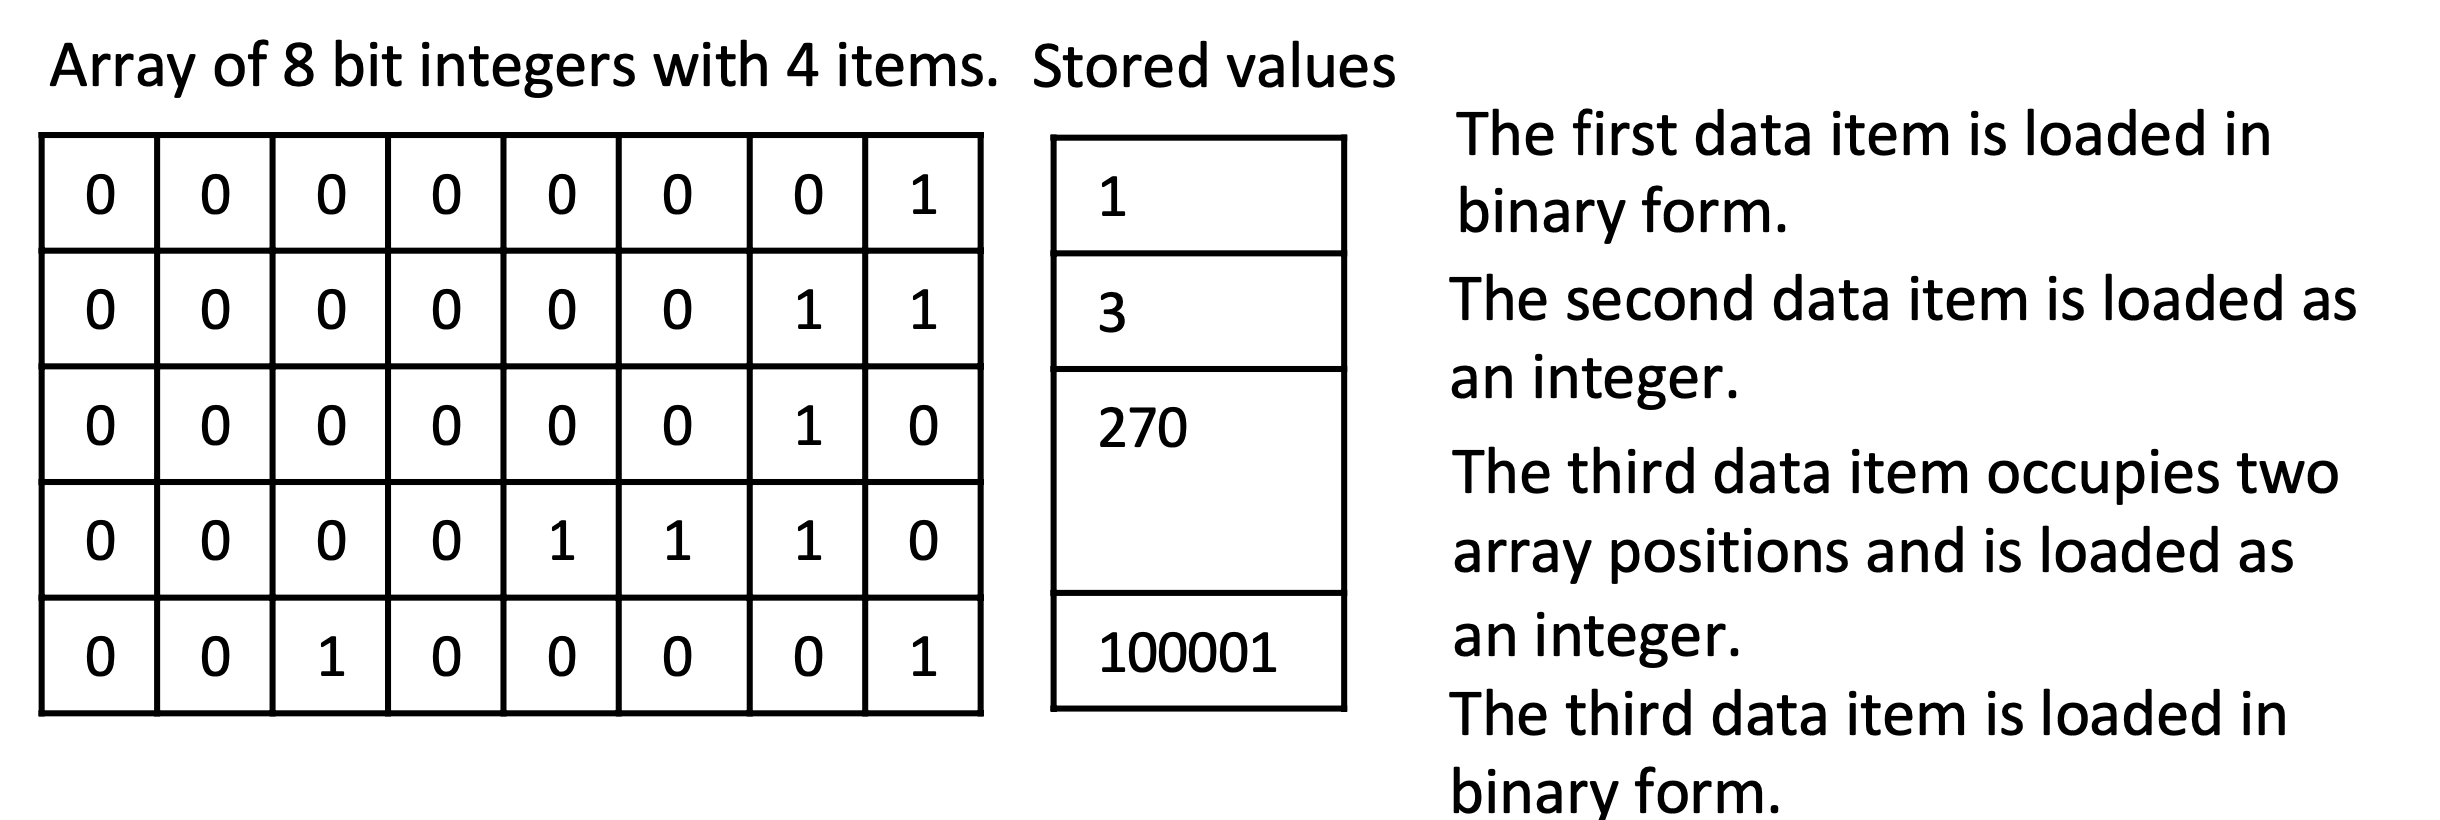
\includegraphics[width=8cm]{damat/images/bufferExample}
%		\caption{Example of a data buffer. \TODO{UPDATE PICTURE}}
%		\label{fig:appr:buffer}
%	\end{figure}

\subsubsection{Fault Modelling Methodology (Step 1)}
\label{sec:methodology}

% !TEX root =  ../MAIN-DataDrivenMutationAnalysis.tex

%
%\setlength\LTleft{0pt}
%\setlength\LTright{0pt}
%\begin{longtable}{@{\extracolsep{\fill}}|p{2.5cm}|p{5cm}|p{5cm}|@{}}
%\toprule


\begin{table}[tb]
\caption{\APPR fault modelling methodology}
\label{table:method}
\center
\scriptsize
\begin{tabular}{|
@{\hspace{1pt}}>{\raggedleft\arraybackslash}p{10mm}@{\hspace{1pt}}|
@{\hspace{1pt}}>{\raggedleft\arraybackslash}p{15mm}@{\hspace{1pt}}|
@{\hspace{1pt}}>{\raggedleft\arraybackslash}p{15mm}@{\hspace{1pt}}|
@{\hspace{1pt}}>{\raggedleft\arraybackslash}p{10mm}@{\hspace{1pt}}|
@{\hspace{1pt}}>{\raggedleft\arraybackslash}p{13mm}@{\hspace{1pt}}|
@{\hspace{1pt}}>{\raggedleft\arraybackslash}p{17mm}@{\hspace{1pt}}|
}
\hline
\textbf{Data} \textbf{nature}&\textbf{Representation} \textbf{type}&\textbf{Dependencies}&\textbf{\# of input} \textbf{partitions}&\textbf{Operators}&\textbf{Comments}\\
\hline
numerical&I, L, F, D&stateless/stateful&2&[VAT,FVAT]&Nominal below T\\
&&&&or [VBT,FVBT]&Nominal above T\\
\cline{4-6}
&&&3 or more&[VOR,FVOR]&\\
\cline{3-6}
&&stateful&&INV&For valid range\\
\cline{4-6}
&& &&[VOR,FVOR]&For out of range\\
\cline{3-6}
&&signal&&ASA, SS, HV&\\
\hline
categorical&I, H&N/A&N/A&IV&\\
\cline{2-6}
%&string&N/A&N/A&BF\\
%\cline{2-5}
&B&N/A&N/A&BF&\\
\hline
ordinal&I, H&N/A&N/A&ASA&\\
\hline
other&B&N/A&N/A&BF&\\
\hline
\end{tabular}\\
\textbf{Legend:} N/A not applicable.
\end{table}
%\normalsize

The fault model shall enable the specification of 
all possible interoperability problems in the SUT while minimizing equivalent and redundant mutants.
Equivalent mutants have the same observable output as the original SUT. 
Instead, redundant mutants have the same observable output as other mutants.
We use the term \INDEX{observable output} to refer to any output that can be verified by the test suite.
The equivalent or redundant nature of a mutant depends
on the equivalence relation for observable outputs
(i.e., how to determine if two outputs are the same).
In a testing context, such equivalence relation depends on the type of testing being performed. For example, system test cases, different than unit test cases,  are unlikely to verify the values of all the state variables of the system and thus mutants that are nonequivalent for unit test suites might be considered equivalent for system test suites. 
For example, in satellite systems, the correctness of the GPS triangulation algorithm output is verified by unit test cases; system test cases, instead, verify 
if the software takes appropriate actions when the satellite is out of orbit. Consequently, slight changes in the coordinates communicated by the GPS component may not lead to any change in the observable output verified by the test suite.
%When defining a fault model, engineers shall thus select and configure mutation operators in such a way that the mutations performed trigger changes in the observable output of the SUT (to avoid equivalent mutants) and (2) distinct mutations do not lead to the same observable outputs (to avoid redundant mutants).


We provide a set of guidelines for the definition of fault models that 
are summarized in Table~\ref{table:method}. 
For guidance,
% are based on the characteristics of the data being exchanged by CPS components.
we account for the nature of the data (i.e., numerical, categorical, ordinal, or binary) and their representation type.
Also, for numerical data, 
we consider 
%the type of measurement, that is, if the data is counted (i.e., it is discrete) or measured (i.e., it is continuous) and
%For numerical data, mutations shall be defined taking into consideration
the data dependencies, that is how data values depend on the previously observed values; we identified three categories: stateless (i.e., there are no dependencies between consecutive values), stateful (i.e, values depend on previous ones), and signal (i.e., values derive from a function of independent variables like time).
\CHANGED{Data dependencies determine the granularity of the mutation (i.e., with data dependencies, small differences shall be noticed); for non numerical data, we do not provide mutation operators with different granularities and data dependencies can be ignored.}
%on previous values and the time in which they are observed).

 

For \INDEX{stateless numerical data}, our guidelines are driven by input space partitioning concepts~\cite{Ammann:Offutt:2008}.
Indeed, given equivalence relations among outputs, it is unlikely that every change in \INDEX{stateless numerical data} will result into nonequivalent mutants; however, we can partition the input domain into regions with equivalent values (partitions).
Precisely, we rely on the  
\INDEX{interface-based input domain modeling} approach~\cite{Ammann:Offutt:2008}:
%Within data-driven mutation analysis, 
for each data item we identify a number of input partitions (set of values or value ranges) according to the interface specifications of the interacting components.
%each data item represents an input partition that shall be split into sets of values (or value ranges) identified according to the interface specifications of the interacting components.
%an input partition corresponds to a single data item and it shall be split into a set of blocks defined according to the interface specifications of the interacting components. 
In our methodology, the number and type of mutation operators selected for stateless numerical data depend on the number of input partitions identified.
With \emph{two input partitions} (e.g., nominal and exceptional data values), engineers can rely either on the pair [VBT,FVBT] or the pair [VAT,FVAT]. 
%Engineers shall select the pair of operators that simplifies the reading of the fault model.
%FABRIZIO: initially, I have explained what I mean with simplyfiy the reading (see below), however, these are details that may not be that necessary in a 10 pages conference paper.
%Engineers shall select the pair of operators that simplifies the reading of the data model; precisely, when the two input partitions capture  ranges for nominal and exceptional data values, the selection depends on how exceptional cases are identified (i.e., below or above the threshold). For other cases (i.e., two input partitions not related to exceptional cases), engineers can select any of the two pairs.
With \emph{three partitions}, engineers must configure one VOR and one FVOR operator. If a different delta (\D) is considered for the upper and lower bounds, engineers may configure two pairs [VBT,FVBT] and [VAT,FVAT], for the lower and upper bound, respectively. In the presence of \emph{more than three} partitions, engineers shall configure one [VOR,FVOR] pair for each extra partition above three (e.g., two pairs in the case of five partitions). The parameter \D{} is used to determine the partition to which the mutated data belongs. 
%Please note that mutants belonging to each pair shall not lead to redundant mutants.
%Engineers can configure multiple [VOR,FVOR] pairs in case several combinations needs to be tested.


In the presence of \INDEX{stateful data}, replacement with random values in the valid range (i.e., the INV operator) will lead to nonequivalent mutants (e.g., because it leads to data values that are systematically different than the values expected for the current system state). Alternatively, the valid data range might be partitioned as for stateless data. However, to avoid redundant mutants, engineers should rely either on the INV operator or the partitioning of the valid data range. 
The effect of data outside the valid data range should instead be verified by means of the [VOR, FVOR] pair.

For \INDEX{signal values}, depending on the shape of the expected signal, engineers should configure one operator among the ASA, SS, and HV. The configuration of more than one of these operators may lead to redundant mutants (e.g., because each of them triggers the same warning in the SUT).

With \INDEX{categorical data} represented using \emph{integers and hexadecimals}, engineers must configure one IV operator for each possible value; indeed, a change in the observed category shall trigger a different behaviour in the SUT. 
%With categorical data represented using labels (e.g., strings), engineers shall configure one BF operator with the MAX parameter set to the minimum number of characters taken by the string; indeed, such a bit flip mutation ensures to alter the transmitted label (e.g., change a characater of the string label) and thus introduce a nonequivalent mutant.
With categorical data in \emph{binary form}, each bit indicates a specific class (e.g., the unit in error for the DataItem2 in the IFStatus message of Figure~\ref{fig:appr:bufferStructure}).  
To verify that the test suite can detect any possible category change, engineers must configure two BF operators for every bit (both MIN and MAX must coincide with the bit position), one operator must flip a bit when it is set (i.e., $\mathit{STATE}=1$), and the last one when it is unset (i.e., $\mathit{STATE}=0$). 
%If only two categories are represented by the data item (i.e., only one bit is used), it is sufficient to configure one BF operator.

For \INDEX{ordinal data}, which is represented by means of either integers or hexadecimals, we suggest to apply the ASA operator with \emph{T} being set to the middle point of the ordinal scale and \D set to the step distance between consecutive data (usually $1$). For data in binary form (e.g., pictures), engineers must configure a BF operator to flip a number of bits  that is sufficient to alter the semantics of the data (e.g., introduce sufficient noise in images).

%, and values are selected from each region.
%
%==> the structure of the input domain in terms of input characteristics. The test engineer creates a partition for each characteristic. The partition is a set of blocks, each of which contains a set of values. From the perspective of that particular characteristic, the values in each block are considered equivalent.



%observable output difference.
%For stateless data, changes in the observable output of the SUT shall be expected when a data item value is replaced with a data item value that belongs to a differ
%
%For visible output we refer to any (e.g., two mutants causing the same failures in the test suite).
%
%We have an equivalent mutant..
%In system and integration test suites (i.e., the ones exercising components interoperability) it is unlikely that any change in the data exchanged by components result in a test case failure. 
% 
%
%Somehow, to make a system test case fail, the granularity of the error observed the data shall be coarser than the one require to make a unit test case fail. In a mutation analysis context this means that, to avoid equivalent mutants (that is 
%
%targeting functional correctness of the results computed after processing
%
%and thus make test cases fail.

% !TEX root = ../MAIN.tex
\begin{table}[h]
\begin{center}
\scriptsize
\begin{tabular}{|p{2cm}|p{2cm}|p{4cm}|p{6cm}|}
\hline
\textbf{Fault Class}&\textbf{Types}&\textbf{Parameters}&\textbf{Description}\\
\hline
Value above threshold (VAT)&
\begin{minipage}{6cm}
INT\\
LONG INT\\
FLOAT\\
DOUBLE
\end{minipage}
&
\begin{minipage}{6cm}
T: threshold\\
D: delta with respect to threshold\\
\end{minipage}
&
\begin{minipage}{6cm}
The value is above a threshold T for a delta D. 

\EMPH{Data mutation operation:} The mutation is performed by replacing the current value (a number) with a value of the same type that is equal to $(T+D)$.
\end{minipage}
\\

\hline
Value below threshold (VBT)&
\begin{minipage}{6cm}
INT\\
LONG INT\\
FLOAT\\
DOUBLE
\end{minipage}
&
\begin{minipage}{6cm}
T: threshold\\
D: delta with respect to threshold\\
\end{minipage}
&
\begin{minipage}{6cm}
The value is below a threshold T for a delta D. 

\EMPH{Data mutation operation:} The mutation is performed by replacing the current value (a number) with a value of the same type that is equal to $(T-D)$.
\end{minipage}
\\



\hline
Value out of range (VOR)&
\begin{minipage}{4cm}
INT\\
LONG INT\\
FLOAT\\
DOUBLE
\end{minipage}
&
\begin{minipage}{4cm}
MIN: minimum valid value\\
MAX: maximum valid value\\
D: delta with respect to minimum/maximum valid value
\end{minipage}
&
\begin{minipage}{6cm}
The value is out of the valid range MIN-MAX. 

\EMPH{Data mutation operations (2):}  The mutation is performed by replacing the current value (a number) with 
\begin{itemize}
\item a value of the same type that is equal to $(MIN-D)$
\item a value of the same type that is equal to $(MAX+D)$
\end{itemize}
\end{minipage}
\\

\hline
Bit flip (BF)&
BIN
&
\begin{minipage}{4cm}
MIN: lower bit\\
MAX: higher bit\\
STATE: mutate only if the bit is in the given state\\
\TRFOUR{VALUE: integer specifying the number of bits to mutate}\\
\end{minipage}
&
\begin{minipage}{6cm}
A number of bits randomly chosen in the positions between MIN and MAX (included) are flipped.

\EMPH{Data mutation operation:} the operator flips N randomly selected bit.
If STATE is specified, the mutation is applied only if  the bit is in the specified state. Parameter VALUE specifies the number of bits to mutate.
\end{minipage}
\\

\hline
Invalid numeric value (INV)&
\begin{minipage}{6cm}
INT\\
LONG INT\\
FLOAT\\
DOUBLE
\end{minipage}
&
\begin{minipage}{4cm}
MIN: lower valid value\\
MAX: higher valid value\\
\TRFOUR{D: distribution to follow}\\
\TRFOUR{VALUE: mean value for normal distribution}\\
\end{minipage}
&
\begin{minipage}{6cm}
The value is legal (i.e., in the specified range) but different than the current one, which, in this case, is expected to be consistent with the status of the system.

\EMPH{Data mutation operation:} Mutation is performed by replacing the current value with a different value randomly sampled in the specified range. The parameter D specified the distribution to follow when performing the mutation\footnote{In our implementation 0 indicates uniform, 1 indicates normal around the specified value (but in range).}
\end{minipage}
\\

\hline
Illegal Value (IV)
&
\begin{minipage}{6cm}
INT\\
LONG INT\\
FLOAT\\
DOUBLE
\end{minipage}
&
\begin{minipage}{6cm}
VALUE: illegal value that is observed\\
\end{minipage}
&
\begin{minipage}{6cm}
The value is illegal and equal to the provided one (i.e., parameter \emph{VALUE}).

\EMPH{Data mutation operation:} Mutation is performed by replacing the current value with the value \emph{VALUE}, if different than the current one.
\end{minipage}
\\

\hline
\TRFOUR{Anomalous Signal Amplitude (ASA)}
&
\begin{minipage}{6cm}
INT\\
LONG INT\\
FLOAT\\
DOUBLE
\end{minipage}
&
\begin{minipage}{6cm}
T: change point\\
D: delta to add/remove\\
V: value to multiply\\
\end{minipage}
&
\begin{minipage}{6cm}
The value is modified by amplifying/reducing it by a factor V and adding or removing D from the observed value. It is used to "amplify" a signal in a constant manner to simulate unusual signal. T indicates the observed value below which instead of adding  we subtract .

\EMPH{Data mutation operation:} Mutation is performed by replacing the current value ($v$) with the value ($v'$) computed as follows:

\[
v' =  
    \begin{cases}
      T+(  (v-T)*V  ) + D   & \mathit{if}\ v \ge T\\
      T - (  (T-v)*V  ) - D   & \mathit{if}\ v < T
    \end{cases}       
\]
\end{minipage}
\\


\hline
\TRFOUR{Signal Shift (SS)}
&
\begin{minipage}{6cm}
INT\\
LONG INT\\
FLOAT\\
DOUBLE
\end{minipage}
&
\begin{minipage}{6cm}
D: delta by which the signal should be shifted\\
\end{minipage}
&
\begin{minipage}{6cm}
The value is modified by adding a value D. It simulate an anomalous shift in the signal.
\end{minipage}
\\





\hline
\TRFOUR{Hold Value (HV)}
&
\begin{minipage}{6cm}
BIN\\
INT\\
LONG INT\\
FLOAT\\
DOUBLE
\end{minipage}
&
\begin{minipage}{6cm}
V: number of times to repeat the same value\\
\end{minipage}
&
\begin{minipage}{6cm}
This operator keeps repeating an observed value for $V$ times. It emulates a constant signal replacing a signal supposed to vary.
\end{minipage}
\\



\hline
\TRFOUR{Array Swap (AS)}
&
\begin{minipage}{6cm}
ARRAY\_*\\
\end{minipage}
&
\begin{minipage}{6cm}
MIN: position of element A\\
MAX: position of element B\\
VALUE: number of elements to move\\
\end{minipage}
&
\begin{minipage}{6cm}
Replace a number of elements (number specified by VALUE) located starting from position MIN, with a number of elements located starting from position MAX, and viceversa.
\EMPH{Data mutation operation:} Mutation is performed by replacing the two set of elements with each other.
\end{minipage}
\\


\hline
\TRFOUR{Array Random Swap (ARS)}
&
\begin{minipage}{6cm}
ARRAY\_*\\
\end{minipage}
&
\begin{minipage}{6cm}
MIN: min position of element A/B\\
MAX: max position of element A/B\\
VALUE: number of elements to move\\
\end{minipage}
&
\begin{minipage}{6cm}
Replace a number of elements (number specified by VALUE) located in a position between MIN and MAX, with a number of elements located in a position between MIN and MAX. MIN and MAX specify a position with respect to the beginning and end of the array.  For example, MIN=0 indicates the first element of teh array, MIN=-2 indicates the second element of the array.
\EMPH{Data mutation operation:} Mutation is performed by replacing the two set of elements with each other.
\end{minipage}
\\



%Incorrect Identifier& Several transmission data fields have fixed values, for example fields identifying the transmitting satellite. Hardware/software errors may assign incorrect identifiers.\\
%%Incorrect Checksum& Hardware/software errors may result in an incorrect checksum for a Packet or VCDU.\\
%Incorrect Counter& Counters are used to track Packet or VCDU ordering. Hardware/software errors may assign incorrect counter values.\\
%Flipped Data Bits& Physical channel noise may flip one or more bits in the data transmission.\\
\hline
\end{tabular}
\end{center}
\caption{Data Fault Classes}
\label{table:faultModel:FAQAS}
\end{table}%

Table~\ref{table:faultModel} provides a specification in tabular form (i.e, the format processed by \APPR) of two fault models configured for the IfKH (i.e., Interface House Keeping) and IfStatus (i.e, Interface Status) messages. In the fault models, each row captures the configuration of a mutation operator for a specific data item. For example, row number 5 indicates that \APPR interprets as double the data inside the two buffer units starting at position 10 (units 10 and 11) and applies the VAT operator. Rows 1 and 2 show that, for a same numerical data item (i.e., the one covering units 8 and 9), we can apply both the VAT and VBT operators, using a different delta for each. 
Rows 2 and 4 show the FVAT and FVBT operators complementing the VAT and VBT operators in rows 1 and 3. They simulate the case in which data for the nominal cases is observed instead of data for exceptional cases, as visible in Table~\ref{table:operators}.
Rows 8 to 23 show that different bits of a same data item can be targeted by different BF operators. %Rows 12 to 14 concern binary categorical data with two categories each, which is the reason why we configured one BF with no STATE setting, according to our methodology. 
\UPDATED{Rows 8 to 13 concern binary categorical data with two categories each, thus we configured two BF each}. 
Rows 14 to 23 concern binary categorical data with five categories; consequently, they present ten BF operators configured for the five categories.
%of DataItem 1.




Figure~\ref{fig:dataMutationFMExamples} provides a visual representation of an array of 8 bit unsigned integers (i.e., unsigned chars) that is modelled using the \EMPH{FMExample} fault model in Table~\ref{table:faultModel:example}. It also provides an example of the mutated data generated by the six mutation operation instances derived from the fault model in Table~\ref{table:faultModel:example}.


% !TEX root = ../MAIN.tex
\begin{table}[h]
\begin{center}
\small
\begin{tabular}{|p{1cm}|p{2cm}|p{1cm}|p{1cm}|p{1cm}|p{1cm}|p{1cm}|p{2cm}|p{1cm}|p{1cm}|}
\hline
\textbf{Fault Model Name}&\textbf{DataItem}&\textbf{Span}&\textbf{Type}&\textbf{Fault Class}&\textbf{Min}&\textbf{Max}&\textbf{Threshold}&\textbf{Delta}&\textbf{State}\\
\hline
IfHK&0&1&BIN&BF&0&0&-&-&-\\
IfHK&1&1&INT&VOR&0&5&-&1&-\\
IfHK&2&2&BIN&BF&0&63&-&-&-\\
IfHK&4&1&BIN&BF&0&0&-&-&-\\
\hline
IfStatus&0&1&BIN&BF&0&0&-&-&-\\
\hline
\end{tabular}
\end{center}
\caption{Driven Fault Model Buffer}
\label{table:faultModel:example}
\end{table}%

\begin{figure}[h]
  \centering
    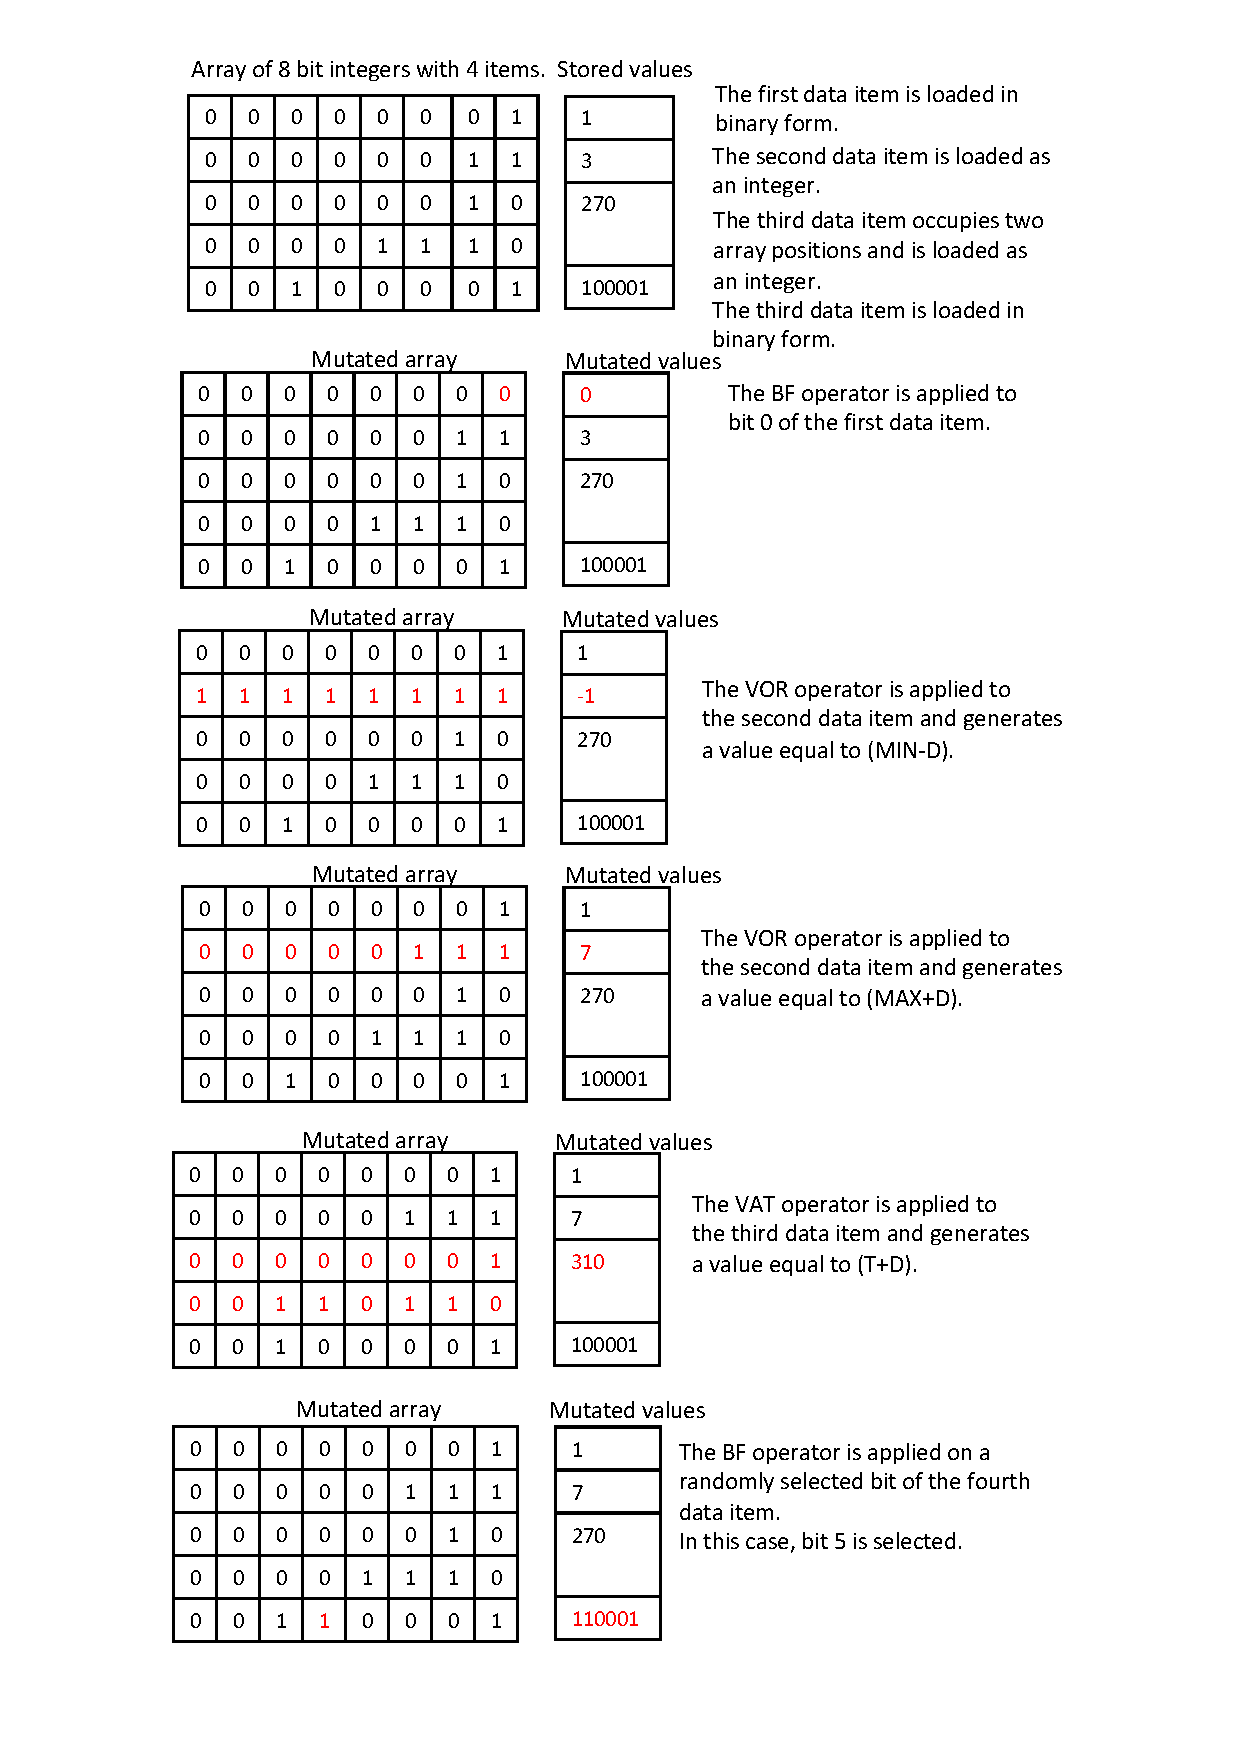
\includegraphics[width=12cm]{images/dataMutationFMExample.pdf}
      \caption{Example of original data and  data mutated according to the fault model in Table~\ref{table:faultModel:example}.}
      \label{fig:dataMutationFMExamples}
\end{figure}





\clearpage


\subsubsection{Automated Generation of Mutation API (Step 2) and Probe Insertion (Step 3)}
\label{sec:generateAPI}

\begin{figure}[tb]
\centering
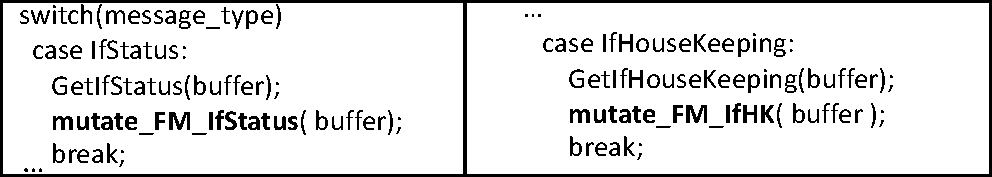
\includegraphics[width=7cm]{damat/images/ProbesExample}
\caption{Example of \APPR mutation probes (in bold).}
\label{fig:appr:ProbesExample}
\end{figure}

\APPR automatically generates a \INDEX{mutation API} to perform mutations at runtime. The API implements a set of functions (called \INDEX{mutate\_FM\_<name>}) that mutate a data buffer according to the given fault model. 
These functions select the data item to mutate and the mutation procedure to apply based on the mutant under test (see Section~\ref{sec:mutantsGeneration}). 

The \APPR mutation API works with C/C++ code; however it may be extended to deal with other programming languages.
Since it is not possible to automatically determine which data buffer to mutate, \APPR requires engineers to modify the source code of the CPS under test by introducing a mutation probe which consists of an invocation of the \APPR function that mutates the data buffer according to a specific fault model.
Note that the effort required by the engineer is minimal; indeed, the exchange of data between components is usually managed in a single location (e.g, the function that serializes the data buffer on the network) and thus it is usually sufficient to introduce one function call for each message type to mutate.
Figure~\ref{fig:appr:ProbesExample} shows how the implementation of \ESAIL has been modified to add the mutation probes. 
The SVF function was modified to handle the message requests sent to the ADCS by inserting one mutation probe for each message type to mutate, e.g., IfStatus and IfHouseKeeping in~Figure~\ref{fig:appr:ProbesExample}. 
Function \emph{mutate\_FM\_IfStatus} is part of the generated mutation API; it loads the fault model \emph{IfStatus} into memory (\UPDATED{our API relies on a tree data structure}) and then invokes the function \emph{mutate}. The function \emph{mutate} performs data-driven mutation according to the provided fault model; the implementation of \emph{mutate} is part of the \APPR toolset.



% At a high-level,
%function \emph{mutate} taking into account the size of the data item; it  checks if the 


The behavior of function \emph{mutate} depends on the value of a unique identifier (i.e., the \emph{MutantID}) associated at compile time to the mutant; the \emph{Mutant ID} univocally identifies the performed mutation operation (each mutant executes one mutation operation, see Section~\ref{sec:mutantsGeneration}).
At a high level, \emph{mutate} performs four activities. First, it checks if the mutation should be performed (i.e., if the data buffer is targeted by the mutation operation identified with the \emph{Mutant ID}). Second, it casts the data item instance targeted by the mutant to a support variable of the type specified in the fault model. Third, it mutates the data stored in the support variable; for each mutation operator, we have implemented a distinct set of instructions for each data representation type. Fourth, before terminating, the function \emph{mutate} writes the mutated data back to the data buffer.





\subsubsection{Automated Generation of Mutants (Step 4)}
\label{sec:mutantsGeneration}



Consistent with code-driven mutation analysis, \APPR generates one mutant for each mutation procedure of the mutation operators configured in the fault model. Each mutant performs exactly one \INDEX{data mutation operation} (i.e., a data mutation procedure configured for a specific data item). For example, the specification in row 6 of Table~\ref{table:faultModel} makes \APPR generate two mutants: each mutant modifies the value of the data item starting at position 12 but one mutant replaces the current value with the value 51 (i.e., $50+1$) while the other replaces the current value with the value $-21$ (i.e., $-20 -1$).

The mutant generation is invisible to the end-user who does not need to modify the source code further; indeed, we rely on a C macro to specify, at compile time, which mutation operation must be performed by every mutant. Mutants are generated by compiling the \UPDATED{SUT} multiple times, once for each mutation operation. At runtime, the mutate function executes only the mutation operation selected for the mutant under test.

\subsubsection{Mutants Execution (Step 5)}
\label{sec:mutantsExecution}

As for \INDEX{code-driven mutation analysis}, the test suite under analysis is executed iteratively with every data-driven mutant. 
At runtime, all the data items targeted by a mutant are mutated whenever the mutation preconditions hold (e.g., the STATE of the BF operator); we leave the mutation of a sampled subset of \UPDATED{data item instances to future work~\cite{zhang2013operator,gopinath2015hard}.}

To speed up the mutation analysis process, the test suite under analysis is first executed with a special mutant that, instead of mutating data items, keeps trace of the fault models loaded by each test case; in other words, it traces what are the data types covered by each test case. The collected information enables the execution, for every mutant, of the subset of test cases that cover the 
message type
%type of data 
targeted by the mutant, thus speeding up mutation analysis.


\subsubsection{Mutation Analysis Results (Step 6)}
\label{sec:mutationAnalysisResults}

Inspired by work on \INDEX{abstract mutation analysis}~\cite{Offutt2006}, we have defined three metrics to evaluate test suites with data-driven mutation analysis: \INDEX{fault model coverage}, \INDEX{mutation operation coverage}, and \INDEX{mutation score}. 
%The first two provide information about the quality of test inputs, whereas the latter provides information about the quality of test oracles \CHANGED{and the test process}. Different from code-driven mutation analysis, data-driven mutation analysis thus enables engineers to distinguish between these two distinct problems affecting test suite effectiveness.
These metrics measure the frequency of the following scenarios: (case 1) the message type targeted by a mutant is never exercised, (case 2) the message type is covered by the test suite but it is not possible to perform some of the mutation operations (e.g., because the test suite does not exercise out-of-range cases), (case 3) the mutation is performed but the test suite does not fail.
\CHANGED{Different from code-driven mutation analysis, these three metrics enable engineers to distinguish between possible test suite shortcomings, including untested message types, uncovered input partitions, poor oracle quality, 
%faulty software, 
and lack of test inputs.}

\INDEX{Fault model coverage (FMC)} is the percentage of fault models covered by the test suite. Since we define a fault model for every 
message type exchanged by two components,
%different data buffer (i.e., type of data exchanged by two components), 
it provides information about the extent to which the message types actually exchanged by the SUT are exercised and verified by the test suites. 
%In other words, low fault model coverage indicates that many test scenarios (e.g., a specific sequence of test inputs being sent to the CPS when the environment is in a specific state) are not exercised by a test suite. 
\CHANGED{Since different component functionalities often require different message types, low fault model coverage may indicate that only a small portion of the integrated functionalities have been tested.}

\INDEX{Mutation operation coverage (MOC)} is the percentage of data items that have been mutated at least once, considering only those that belong to the data buffers covered by the test suite. It provides information about the input partitions covered for each data item; for example, the FVOR operator leads to two mutation operations, which are applied only if the observed value is outside range. Otherwise the two mutation operations will not be covered, thus enabling the engineer to identify such shortcoming in the test suite.
%TODO: add example

The \INDEX{mutation score (MS)} is the percentage of mutants killed by the test suite \UPDATED{(i.e., leading to at least one test case failure)} among the mutants that target a fault model and for which at least one mutation operation was successfully performed. It provides information about the quality of test oracles; indeed, a mutant that performs a mutation operation and is not killed (i.e., is \emph{live}) indicates that the test suite cannot detect the effect of the mutation (e.g., the presence of warnings in logs).
% or an unexpected output from the system). 
\CHANGED{Also, a low mutation score may indicate missing test input sequences. Indeed, live mutants may be due to either software faults (e.g., the SUT does not provide the correct output for the mutated data item instance) or the software not being in the required state (e.g., input partitions for data items are covered when the software is paused); in such cases, with appropriate input sequences, the  test suite would have discovered the fault or brought the SUT into the required state. Both poor oracles and lack of inputs indicate flaws in the test case definition process (e.g., the stateful nature of the software was ignored).}

\clearpage
\subsection{Running Examples}
\label{sec:dataDriven:example}

In this Section, we provide a set of running examples that show the results achieved by \APPR in the presence of test suites affected by different problems. More precisely we aim to demonstrate, for representative cases, the absence of false alarms due to equivalent mutants and the usefulness of the mutation analysis metrics computed. 
\REVTOOL{P-3}{Each running example is an artificial but realistic definition of test suites to illustrate the methodology.}
We consider the following representative scenarios:
\begin{enumerate}
\item The test suite exercises only one message exchange between the ADCS and the SUT; each test case covers a distinct input partition.
\item The test suite exercises only one message exchange between the ADCS and the SUT; multiple test cases cover a same input partition.
\item The test suite exercises multiple message exchanges between the ADCS and the SUT; each test case covers a distinct combination of input partitions.
\end{enumerate}


\subsubsection{Example set 1: One message exchange, distinct input partitions}
\label{sec:dataDriven:example:1}

\begin{figure}[tb]
\centering
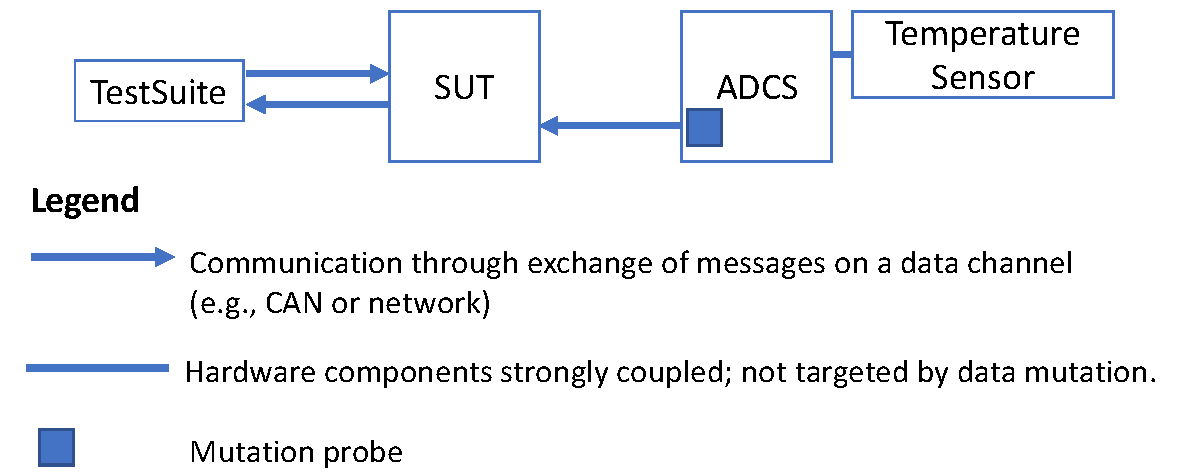
\includegraphics[width=8cm]{damat/RunningExampleArch}
\caption{Architecture of the running example system.}
\label{fig:damat:RunningExampleArch}
\end{figure}

Our first set of running examples concerns the presence of a single message exchange and test cases covering distinct input partitions.

Our examples concern an SUT that exchanges with the ADCS component one type of message. More precisely, the ADCS sends a message (hereafter, \emph{TempMessage}) with the temperature collected by its sensor. The architecture of such system is shown in Figure~\ref{fig:damat:RunningExampleArch}. For simplicity, we assume that the ADCS periodically sends a TempMessage to the SUT. The ADCS is connected to the TemperatureSensor. The communication between the ADCS and the TemperatureSensor is not affected by data-driven mutation. We may assume the ADCS and the TemepratureSensor are simulated during the execution of the test suite. The SUT and the ADCS communicate through a channel 
(e.g., a CAN bus). The data mutation probe is inserted in the ADCS simulator; in practice we mutate the data generated by the ADCS. The test suite exercises the software under test by communicating through a data channel; the type of communication channel used by the test suite is not relevant for the purpose of the running example.

For our running example, the SUT has two state variables that are observable by the test suite, \emph{temperature} and \emph{temperature\_alarm}. The state variable \emph{temperature} reports the temperature returned by the sensor in the last message. 
The state variable \emph{temperature\_alarm} is set to 1 if the temperature returned by the sensor is above 100.

The test suite is comprised of two test cases. \emph{Test 1} exercises the SUT with a temperature in the nominal case (i.e., temperature below 100), \emph{Test 2} concerns the non nominal case (i.e., temperature above 100). The two test cases of the test suite exercise the same sequence of interactions, which are depicted in the UML Sequence diagram of Figure~\ref{fig:damat:RunningExample1Sequence}. The sequence diagram shows that the test case first starts the ADCS simulator and the SUT; then, it waits for the ADCS to send the TempMessage before requesting the values of the variables \emph{temperature} and \emph{temperature\_alarm}. Figure~\ref{fig:damat:RunningExample1Sequence} also shows that, in this case, the mutation is performed within the ADCS simulator.

\begin{figure}[tb]
\centering
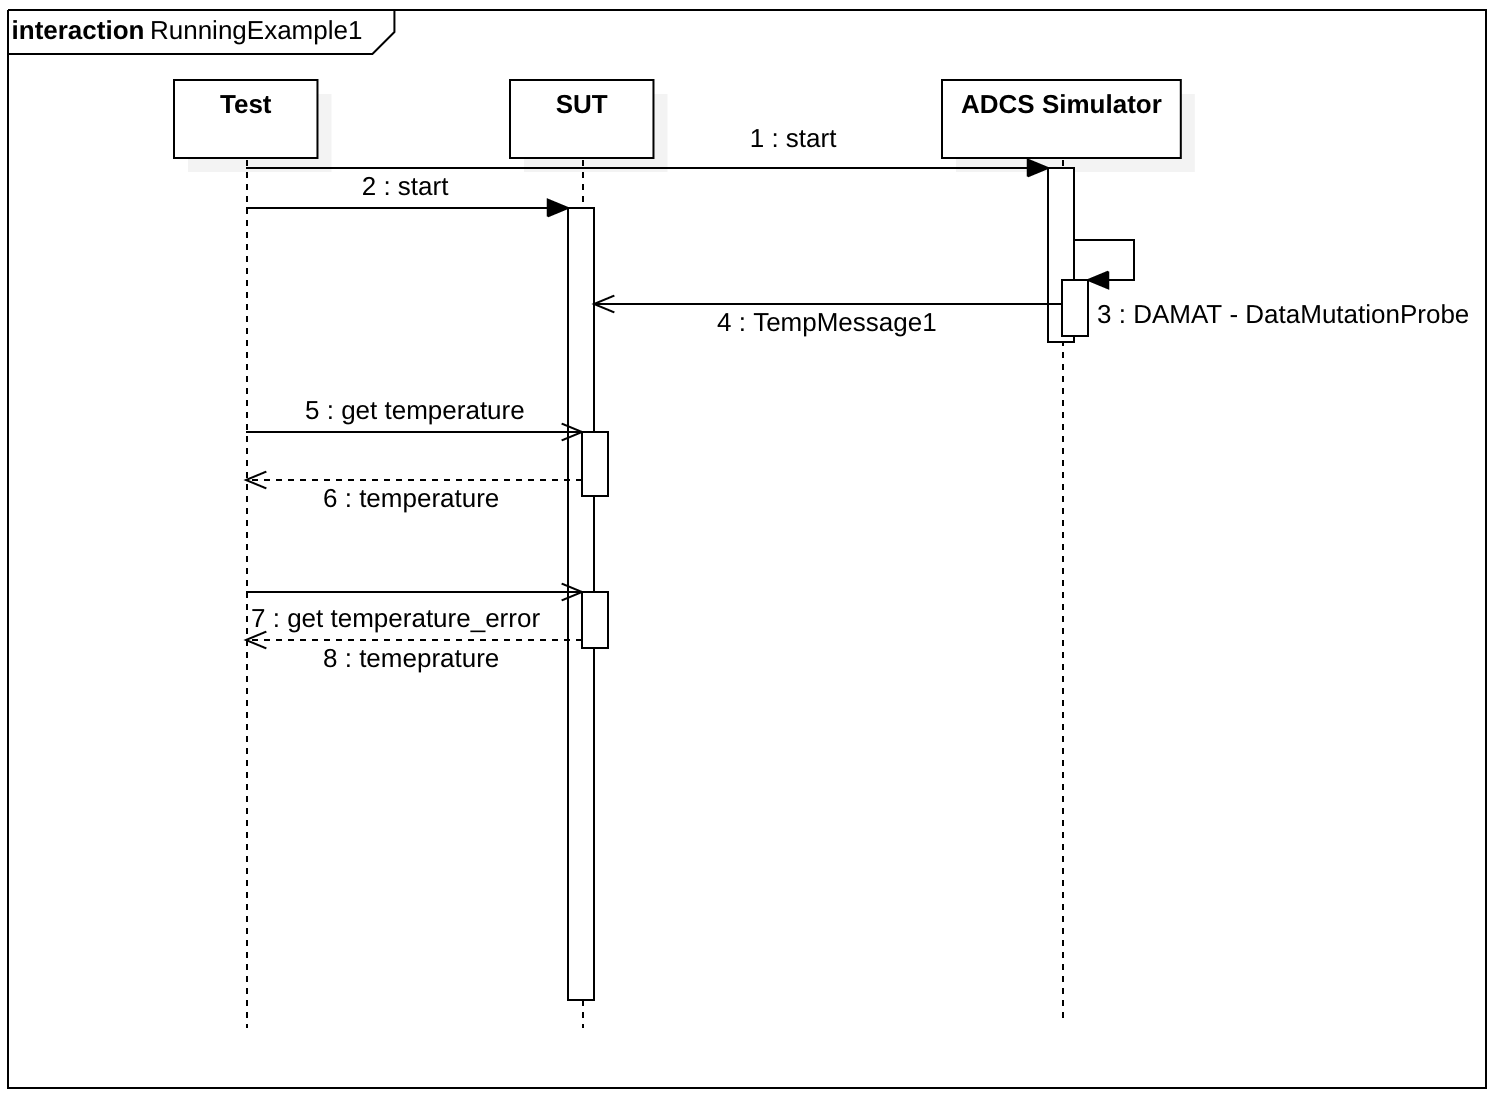
\includegraphics[width=8cm]{damat/images/runningExamplesSequence1.png}
\caption{Interactions exercised by the test cases belonging to the running example set 1.}
\label{fig:damat:RunningExample1Sequence}
\end{figure}


Figures~\ref{fig:damat:RunningExample1A} to~\ref{fig:damat:RunningExample1C} show our running examples. On the top, we report the fault model. In this case the fault model applies the operators VAT (value above threshold) and FVAT (fix value above threshold). The VAT operator is configured with a threshold of 100 and a delta of 10 (i.e., it replaces values below the threshold with the value 110). The FVAT operator is configured in the same manner (i.e., it replaces values above threshold with the value 90). The operator VAT leads to \emph{MUTANT 1}, the operator FVAT leads to \emph{MUTANT 2}; \REVTOOL{P-5}{to summarize, in this example we have two mutants, each implements one distinct mutation operator.}

In Figure~\ref{fig:damat:RunningExample1A}, under \emph{Exchanged data}, we report the sequence of data messages exchanged by the test cases of the test suite (one column for each test case).
In the following rows, we report the oracles. For each oracle we indicate how it verifies if a state variable has been assigned with a correct value; we indicate $"=="$ if it verifies the exact value taken by the state variable (e.g., \emph{temperature == 50)}, "$>=$" if it verifies that the value is above a threshold (e.g., \emph{temperature $>=$ 50}). Please note that, according to standard practice, test cases for non nominal cases verify that state variables contain the expected alarm and anomalous values (i.e., the test case passes only if the SUT report the anomaly). 

For each mutant, we report the value of the data exchanged during the execution and the data of the state variables read by the oracle. In red we indicate data that has been mutated according to the fault model. 
If an oracle does not read the value of a variable we leave the cell empty.
Failing oracles are highlighted in yellow.
\REVTOOL{P-5}{Note that for each mutant we provide multiple columns (named \emph{Test 1} and \emph{Test 2}), each provides the data exchanged during the execution of the test case.}
Finally, for each mutant, for each oracle, we report the test cases that detect the anomalous value (if any); also, we report if the mutant had been killed.


Please note that, following the \APPR procedures, MUTANT 1 does not mutate the data exchanged by Test 2 because it is already above the threshold. MUTANT 2 does not mutate the data exchanged by Test 1 because it is already below the threshold.

TestSuite1 is an optimal test suite that verifies the expected value of all the state variables. For MUTANT 1, Test 1 fails because the assertion about temperature fails (expected 50 observed 110).
For MUTANT 2, Test 2 fails because the assertion about temperature fails (expected 120 observed 90).
\REVTOOL{P-6}{We have a fault model coverage (\emph{FMC}) of 100\% because we have only one fault model and it is covered (i.e., the test suite exchanged the data message under analysis). We have a mutation operator coverage (\emph{MOC}) of 100\% because all the mutation operations associated with the configured mutation operators are applied (in other words, all the mutants perform at least one mutation of a data item instance). We have a mutation score (\emph{MS}) of 100\% because, for each mutant, at least one test case fails.}

TestSuite2 verifies the expected value of the temperature for the nominal case and the presence of a temperature error for the non nominal case. For MUTANT 1, Test 1 fails because the assertion on temperature fails (expected 50 observed 110).
For MUTANT 2, Test 2 fails because the assertion on temperature errors fail (expected 1 observed 0).
\REVTOOL{P-6}{Concerning FMC, MOC, and MS, the same considerations made for TestSuite1 hold.}

TestSuite3 verifies only temperature values while TestSuite4 verifies only temperature alarms. They all kill the mutants for the same reasons reported in the cases above. \REVTOOL{P-6}{Concerning FMC, MOC, and MS, the same considerations made for TestSuite1 hold.}


TestSuite5 is a copy of TestSuite2 having an imprecise oracle (i.e., it verifies that temperature is above 50 instead of equal to 50). Consequently the test suite does not fail for MUTANT 1 and the mutation score is not 100\%; consequently, \APPR enables an engineer to detect the limitation of the test suite.

\REVTOOL{P-6}{TestSuite6} is a copy of TestSuite2 without an oracle for Test2 (i.e., it does not verify the presence of temperature alarms). Consequently, the test suite does not fail for MUTANT 2 and the mutation score is not 100\%; consequently, \APPR enables an engineer to detect the limitation of the test suite.

TestSuite7 is a copy of TestSuite2 with multiple test cases covering the same input partitions; indeed, Test3 covers the same input partition of Test1 (i.e., it exercises the value 0, which is a nominal value like 50), Test4 covers the same input partition of Test2 (i.e., it exercises the value 101, which is a non nominal value like 120). All the mutants are killed by the test suite and we do not observe equivalent mutants.

TestSuite8 is a copy of TestSuite7 with the same limitations of TestSuite6 (i.e., Test2 does not contain an oracle).
In this case, the mutation score is 100\% because Test 4 contains an appropriate oracle and covers the same input partition not appropriately verified by Test 2. We do not observe equivalent mutants.

TestSuite9 is a copy of TestSuite7 without oracles for both Test2 and Test4; similarly to the case of TestSuite6, since the non-nominal partition is not appropriately verified, the mutation score is not 100\%; consequently, \APPR enables an engineer to detect the limitation of the test suite.

TestSuite10 covers the case of a test suite that does not exercise an input partition; precisely, it does not exercise non nominal values. 
In this case, \APPR can detect that MUTANT 2 is never applied (to exemplify it, we do not report any red value for MUTANT 2 in Figure~\ref{fig:damat:RunningExample1C}); consequently, the MOC is not 100\% and the engineer can determine what is the limitation of the test suite. Indeed, since the mutant not covered is FVAT, the engineer can know that the test suite does not exercise the value above threshold for the temperature (FVAT applies the mutation only if a value above threshold is observed).

\begin{figure}[tb]
\centering
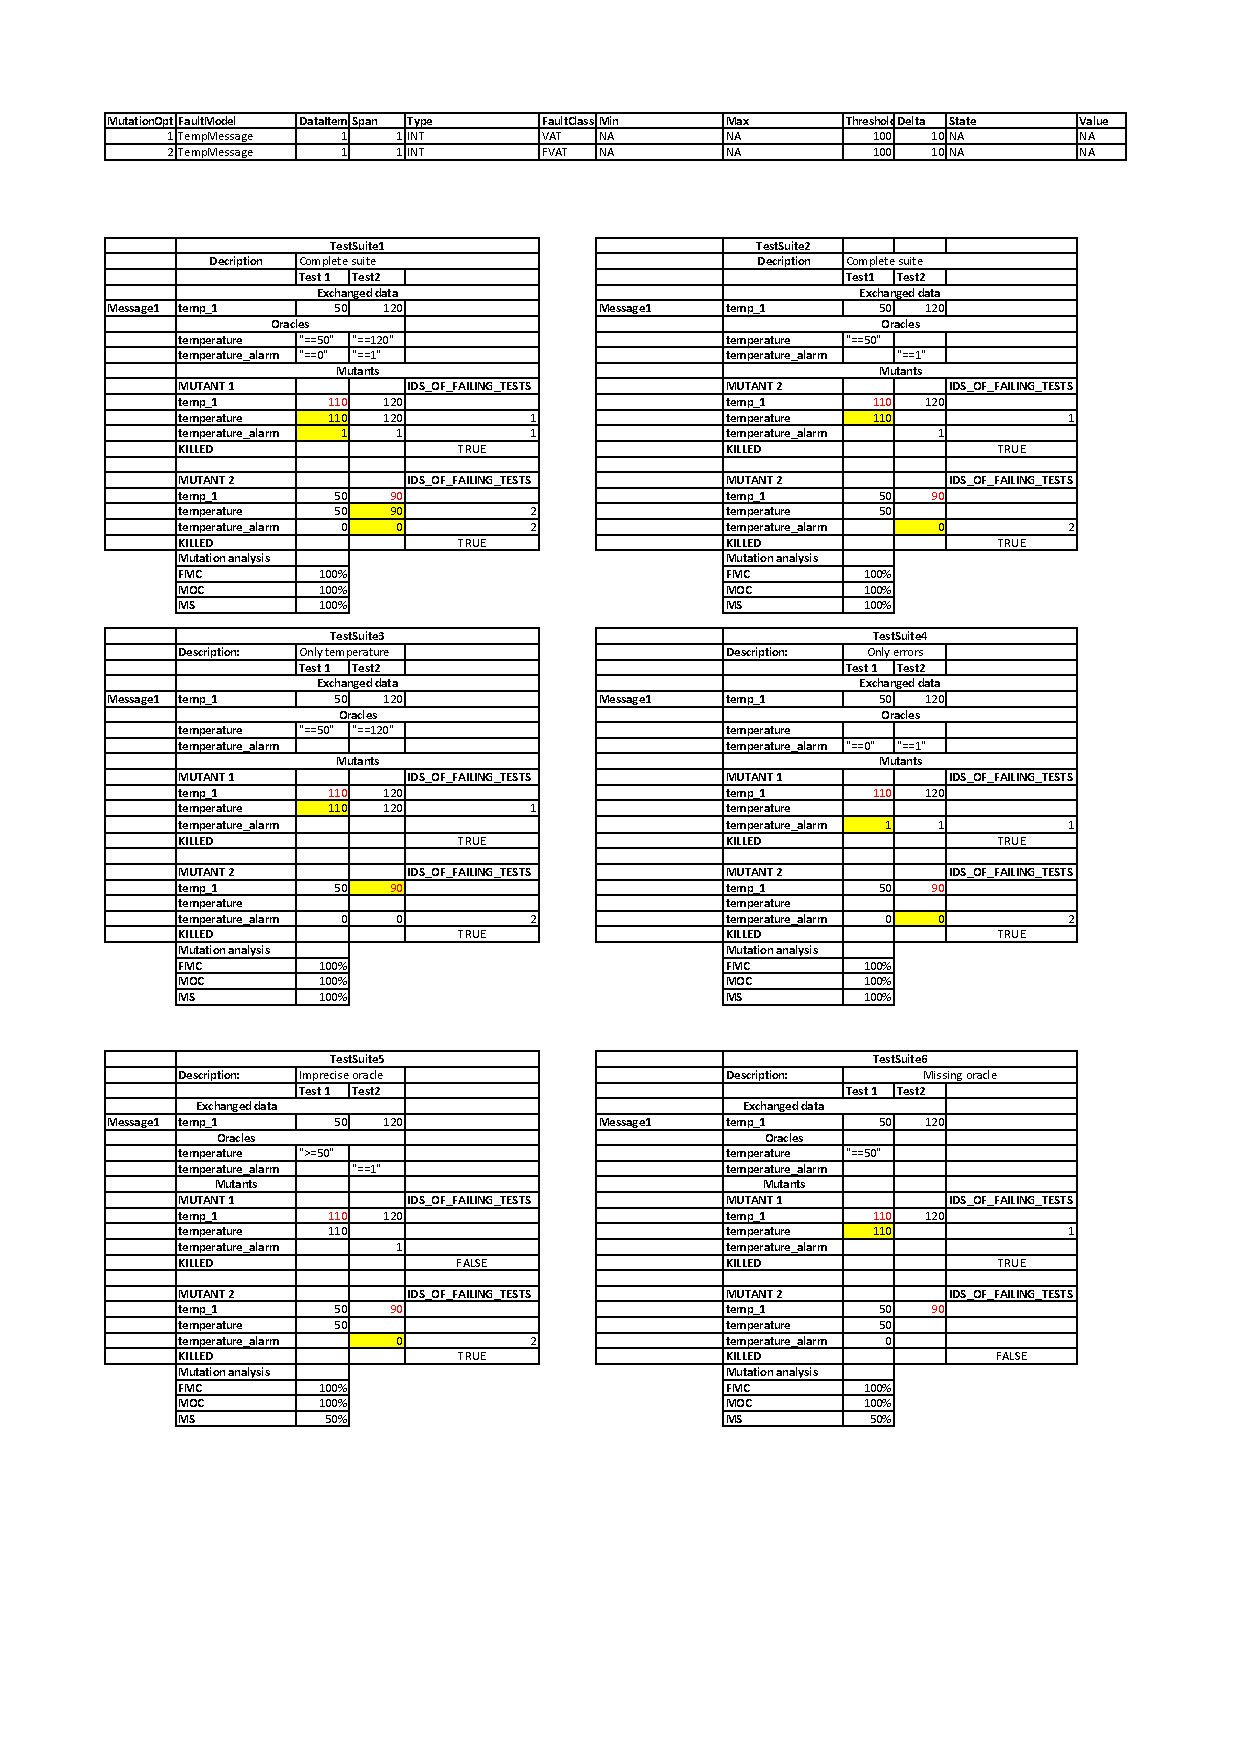
\includegraphics[width=18cm]{damat/DataDrivenExample1A}
\caption{Running example set 1 - Part A.}
\label{fig:damat:RunningExample1A}
\end{figure}

\begin{figure}[tb]
\centering
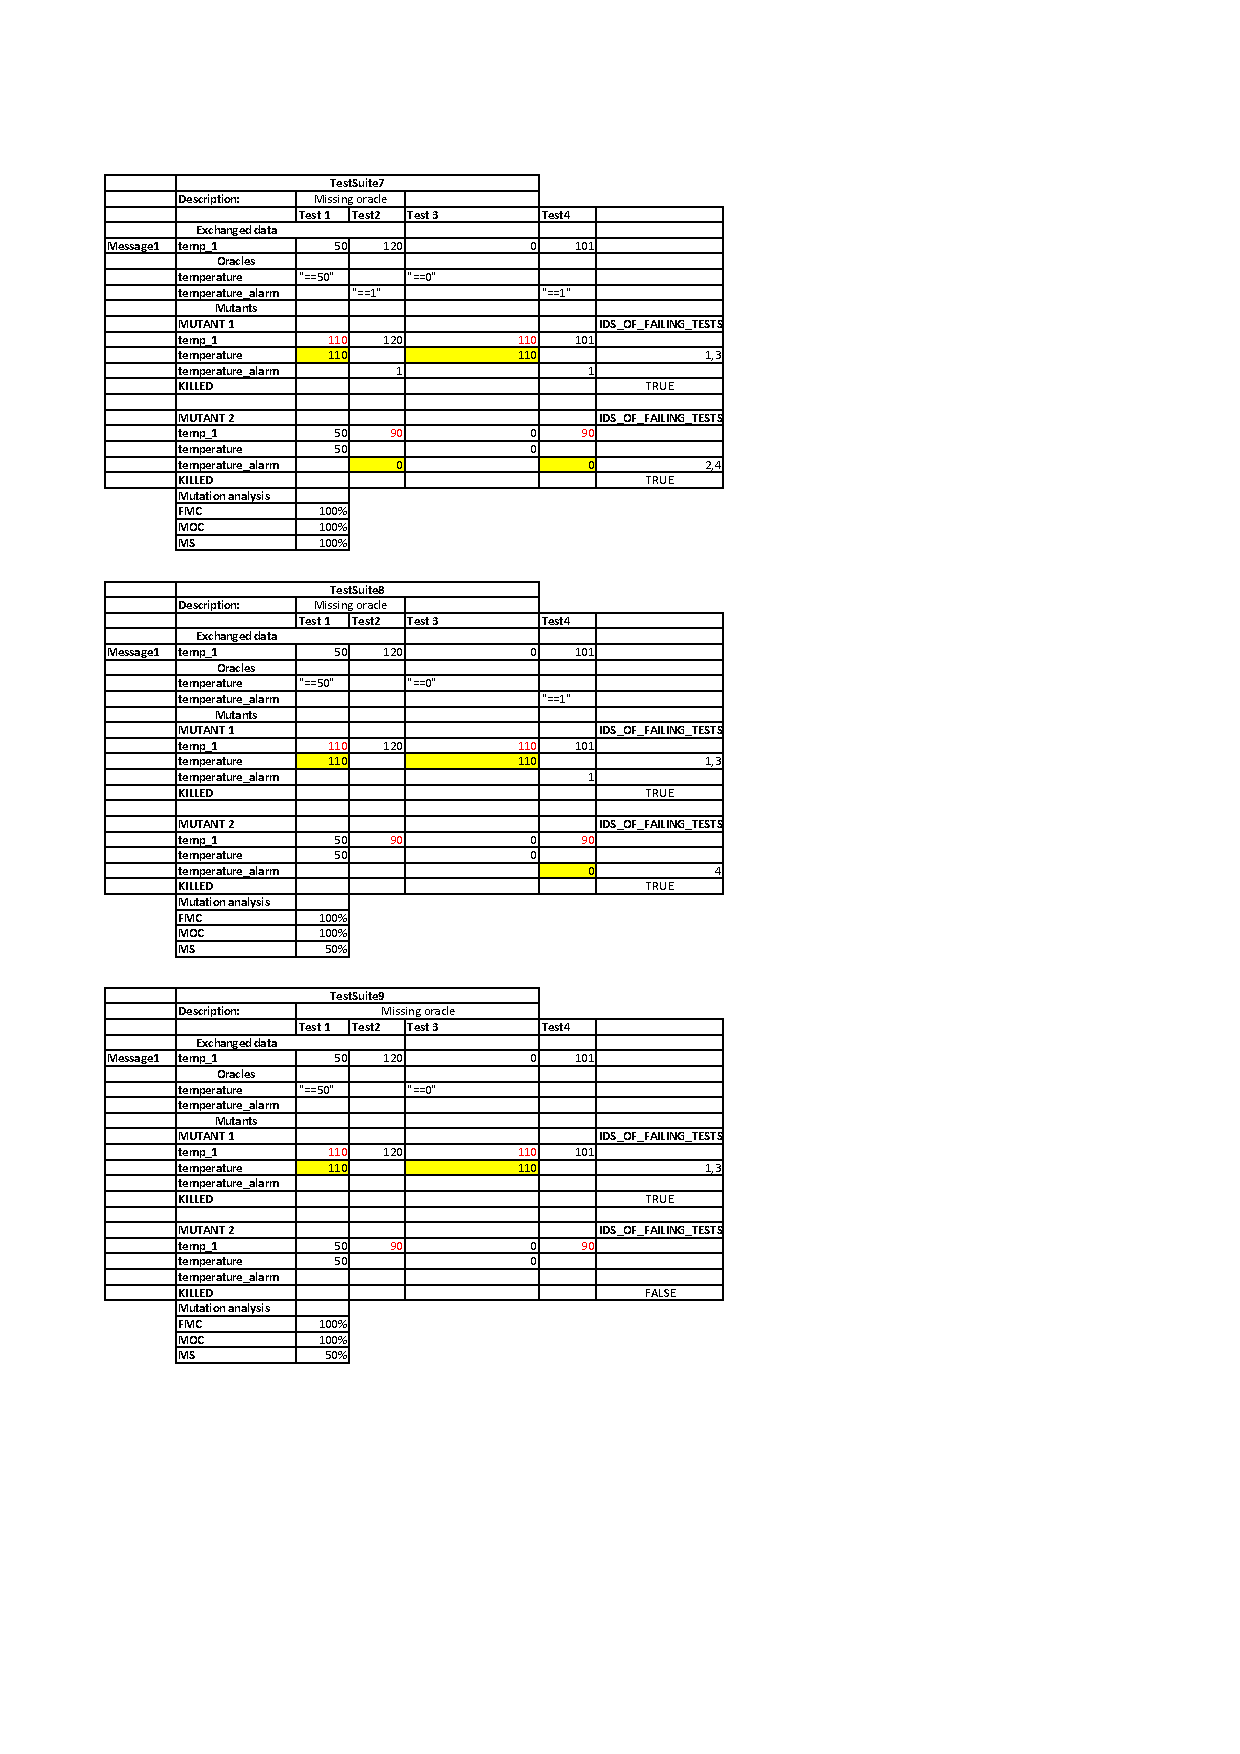
\includegraphics[width=18cm]{damat/DataDrivenExample1B}
\caption{Running example set 1 - Part B.}
\label{fig:damat:RunningExample1B}
\end{figure}

\begin{figure}[tb]
\centering
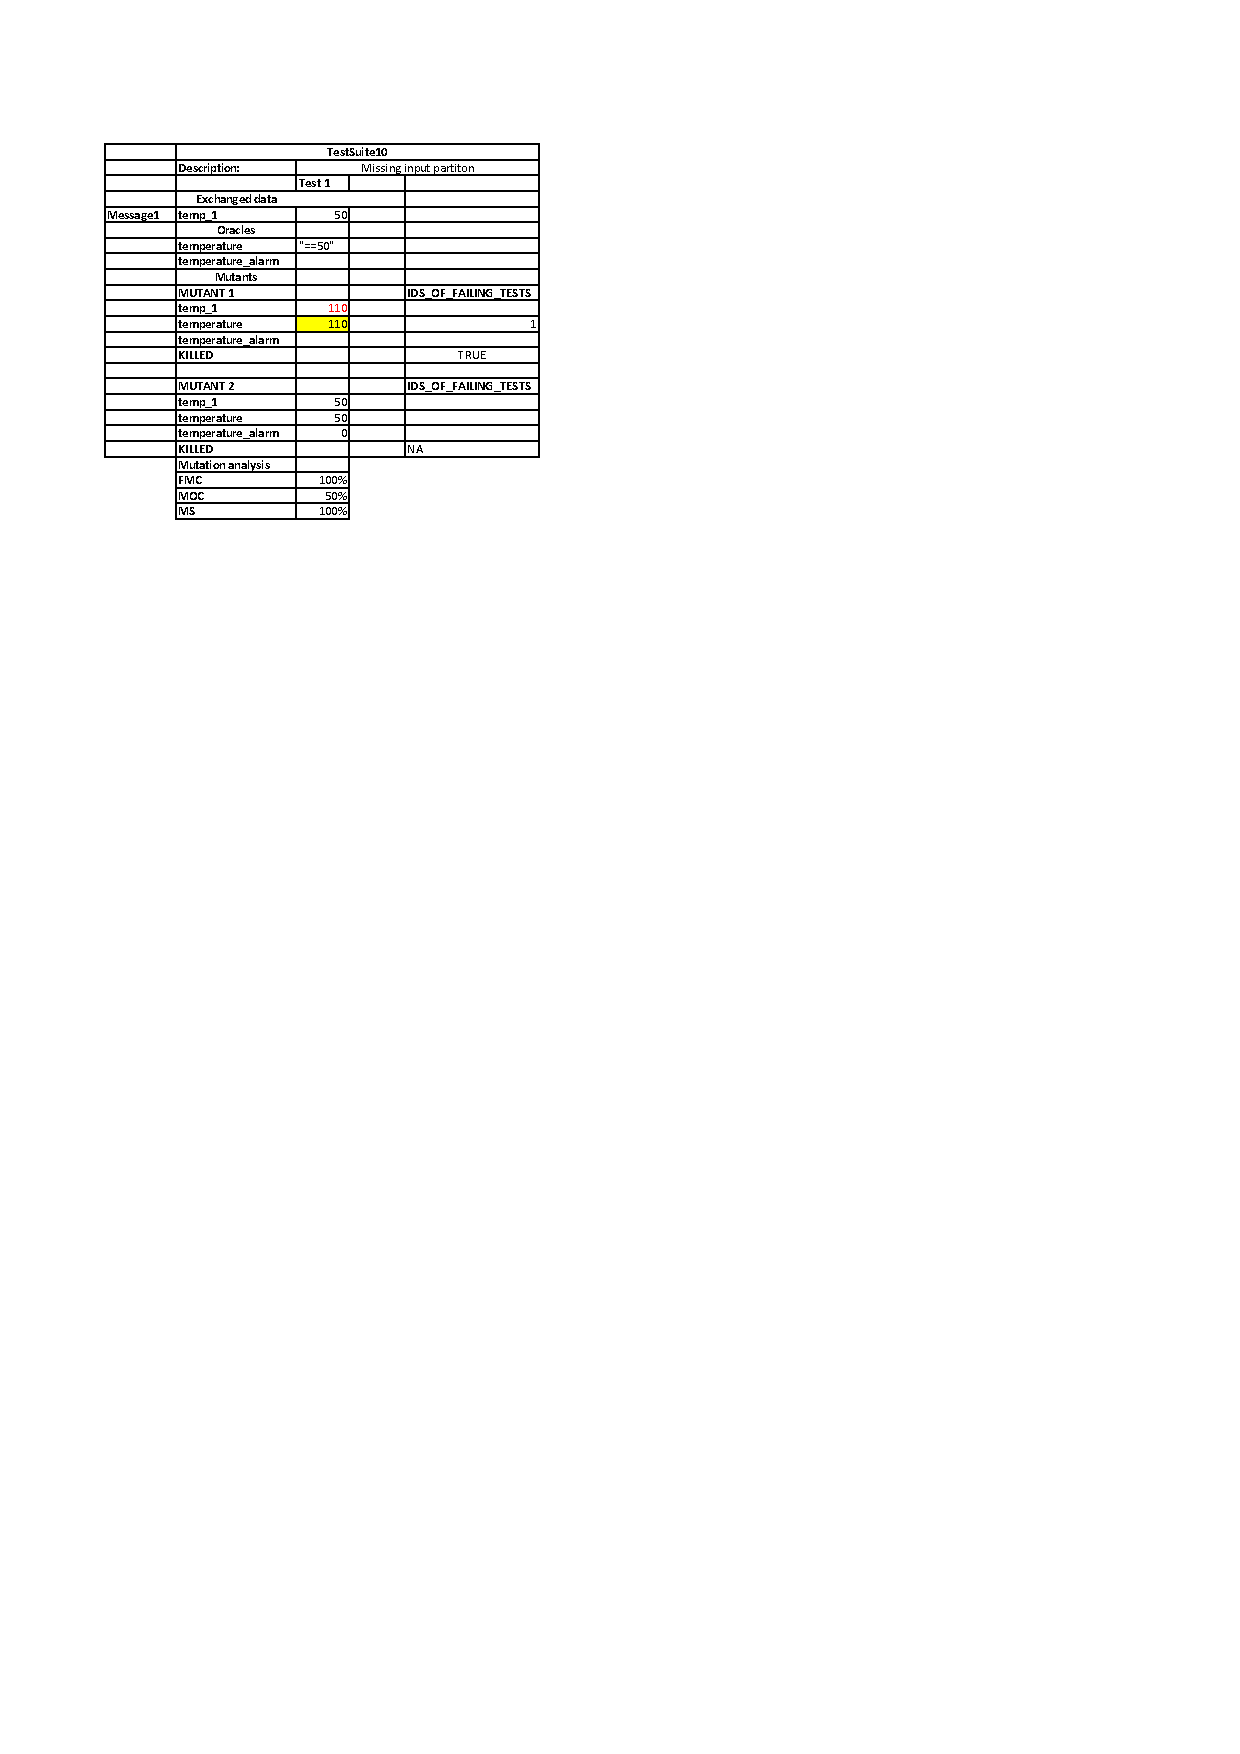
\includegraphics[width=18cm]{damat/DataDrivenExample1C}
\caption{Running example set 1 - Part C.}
\label{fig:damat:RunningExample1C}
\end{figure}

%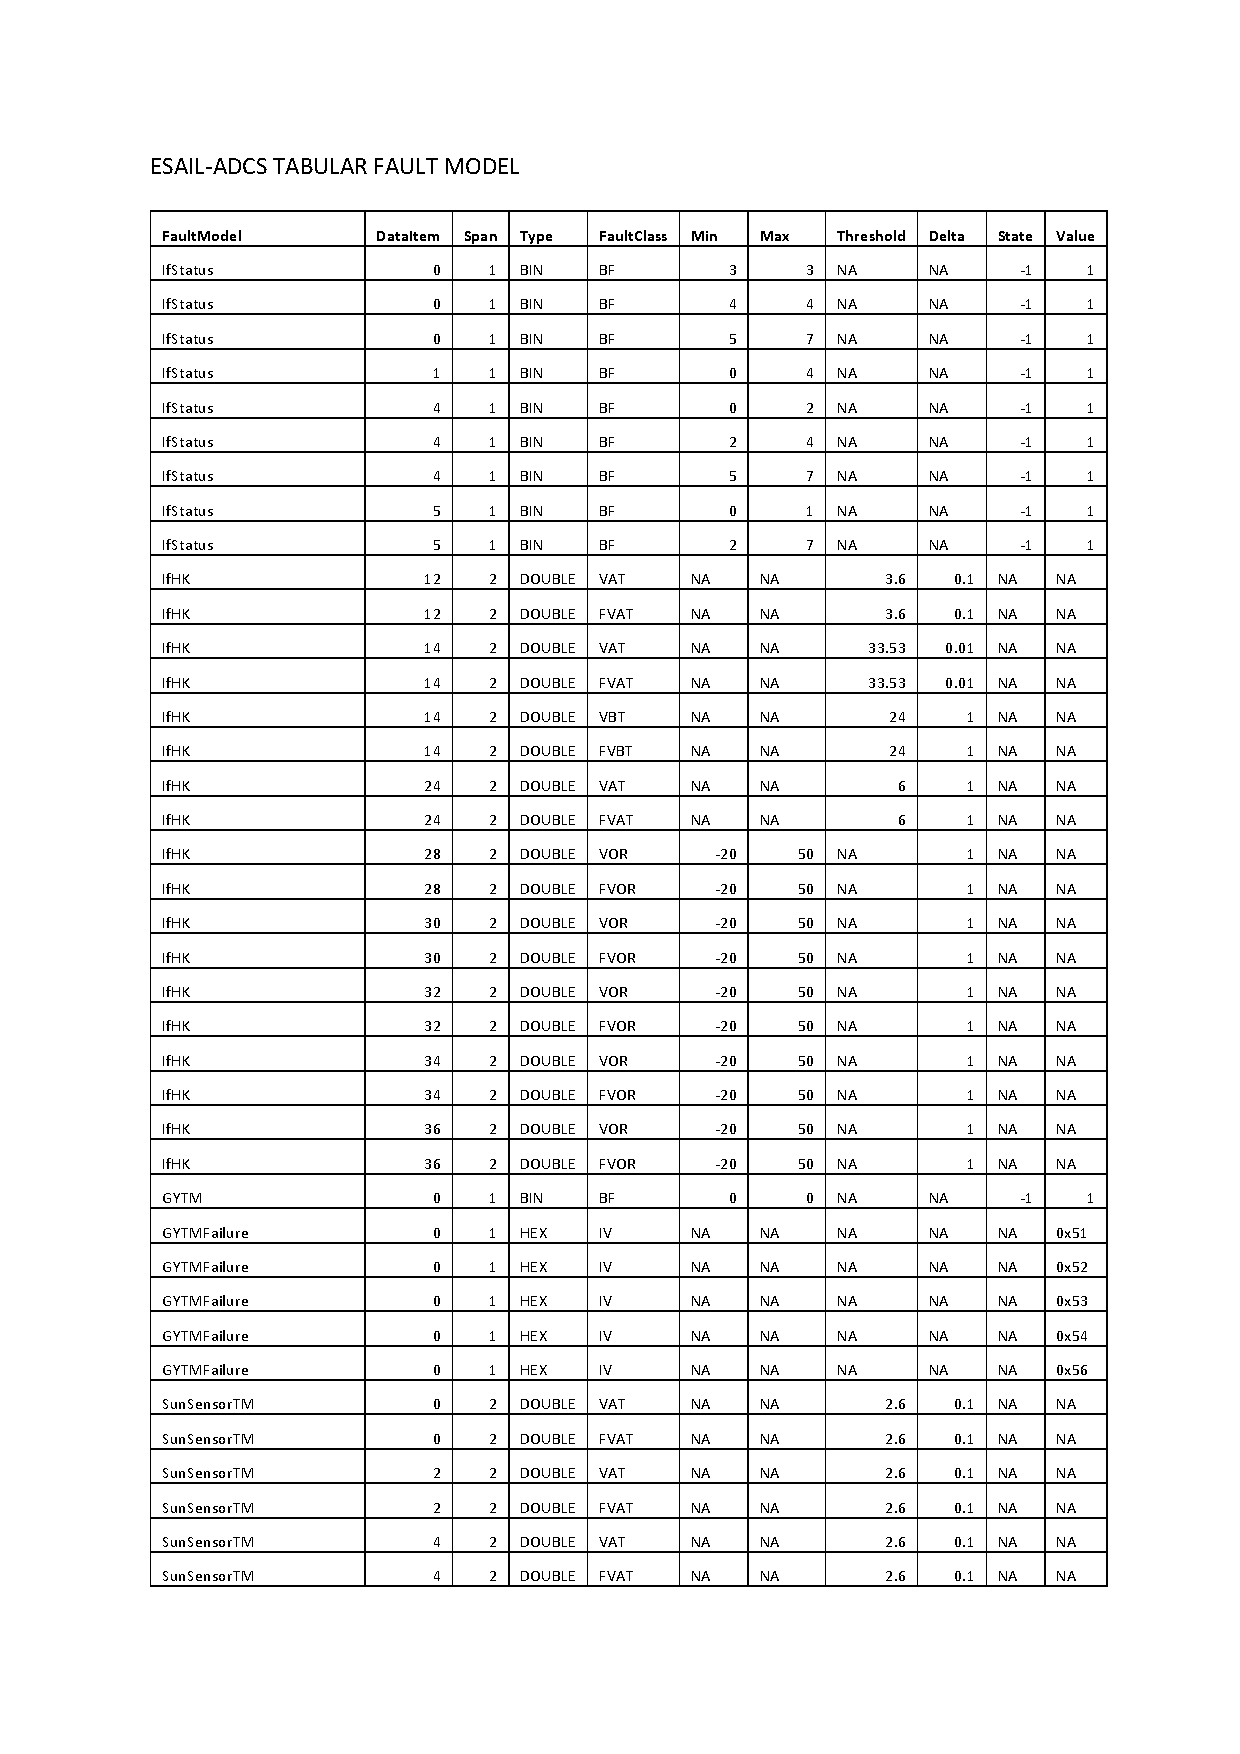
\includepdf[pages=-,scale=0.9,offset=0mm -75]{faultModels/FaultModels.pdf}

\clearpage

\subsubsection{Example set 2: One message exchange, distinct input partitions, faulty software}
\label{sec:dataDriven:example:2}

This running example (see Figure~\ref{fig:damat:RunningExample2}) covers the same case of Section~\ref{sec:dataDriven:example:1}, with the difference that we assume the software to be faulty. More precisely, we assume that the value of \emph{temperature alarm} is always set to 0. We ignore the test suites number 1, 2, 4, 5, 6, 7, 8 because they would detect the presence of the fault before mutation analysis (i.e., the oracles "==1" would fail). For completeness, in Figure~\ref{fig:damat:RunningExample2}, we report the values of state variables also when they are not verified by oracles. We highlight failing oracles in yellow.

For TestSuite6 and TestSuite9, which do not detect the fault because they lack an oracle for the faulty variable, \APPR would indicate that MUTANT 2 is not killed thus enabling the engineer to introduce an appropriate oracle (i.e., "temperature\_alarm == 1") and thus discover the fault. 

For TestSuite3, \APPR would not help the engineer in detecting the fault because the test suite kills the mutant. What we observe in this case is a sort of masking effect due to the fact that two outputs are affected by the same data; indeed, \APPR ensures that the effect of data mutation is propagated to at least one software output but it cannot verify that the effects of data mutation are propagated to all the software outputs that depend on the mutated data. 
%In this specific case, we would like to highlight that a correct test case would have verified first the presence of temperature_alarms. 
%For the detection of algorithmic faults, code-driven mutation analysis might be more appropriate.

\begin{figure}[tb]
\centering
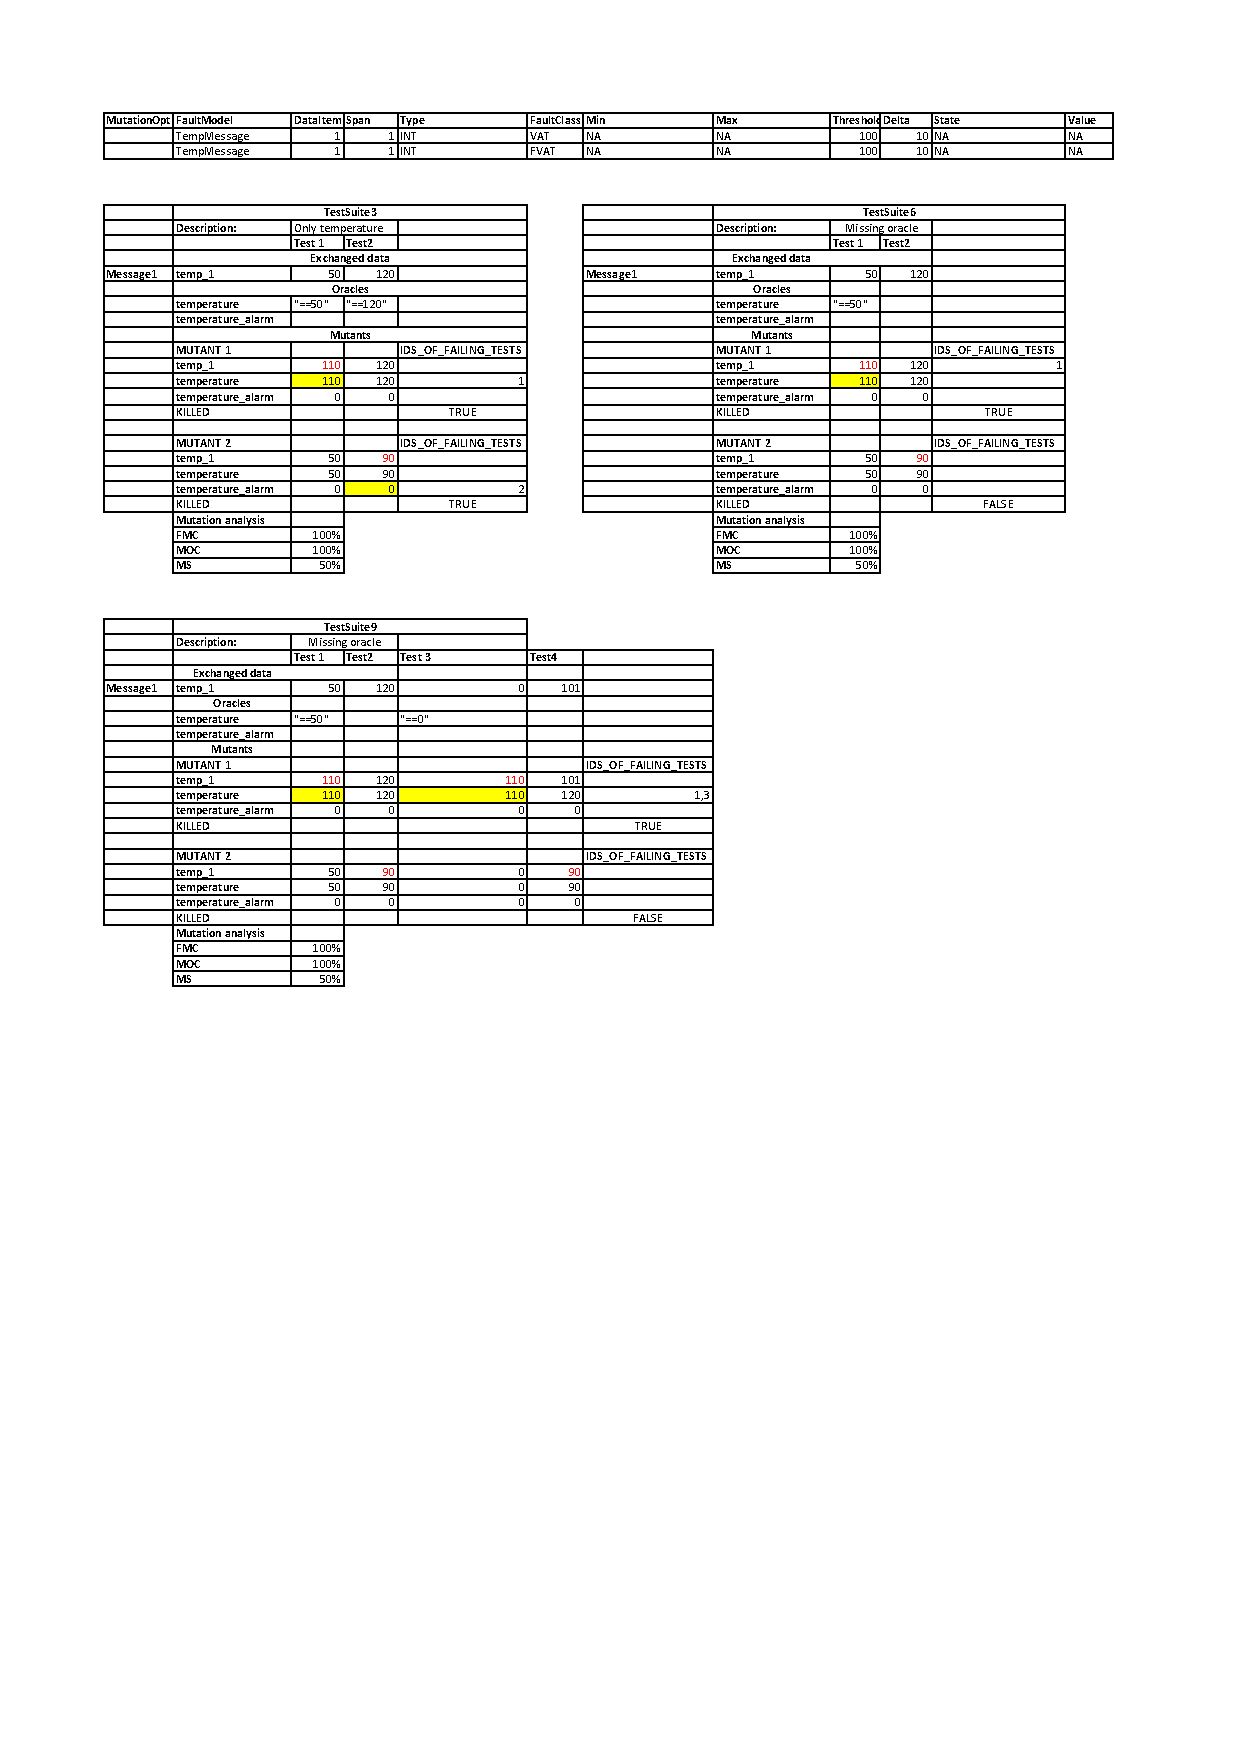
\includegraphics[width=14cm]{damat/DataDrivenExample2}
\caption{Running example set 2.}
\label{fig:damat:RunningExample2}
\end{figure}

\clearpage 
\subsubsection{Example set 3: Multiple message exchanges, distinct input partitions}
\label{sec:dataDriven:example:3}

For the third running example set, we consider a system that has the same architecture of  Figure~\ref{fig:damat:RunningExampleArch} but exchanges also messages of type \emph{BoardStatus}. We assume that \emph{BoardStatus} messages indicate the voltage of the board and the sensors. The SUT has an additional output state variable called \emph{voltage\_error}. A voltage error occurs when the voltage is out of the range (10;14). In the presence of a voltage error, the software shall not update the value of the \emph{temperature} state variable.

Below we discuss two possible test suites, TestSuite1 and TestSuite2, which are affected by different type of limitations.
More precisely, we rely on TestSuite1 to (1) show how \APPR spot a test suite shortcoming difficult to determine manually and (2) demonstrate that \APPR may unlikely lead to equivalent mutants (i.e., by showing that if a mutant is not killed it's because relevant assertions are missing). We rely on TestSuite2 to exemplify the case of lack of coverage of a fault model.

\paragraph{TestSuite1}

Figure~\ref{fig:damat:RunningExample3Sequence} shows the interactions exercised by the test cases in the test suite named TestSuite1 for the running example set 3. Each test case, after starting the ADCS simulator and SUT, waits till the ADCS has sent the following sequence of messages: one BoardStatus message, one TempMessage, one BoardStatus message, and one TempMessage. Then it requests and verifies the values of the state variables \emph{temperature}, \emph{temperature\_alarm}, and \emph{voltage\_error}.

\begin{figure}[tb]
\centering
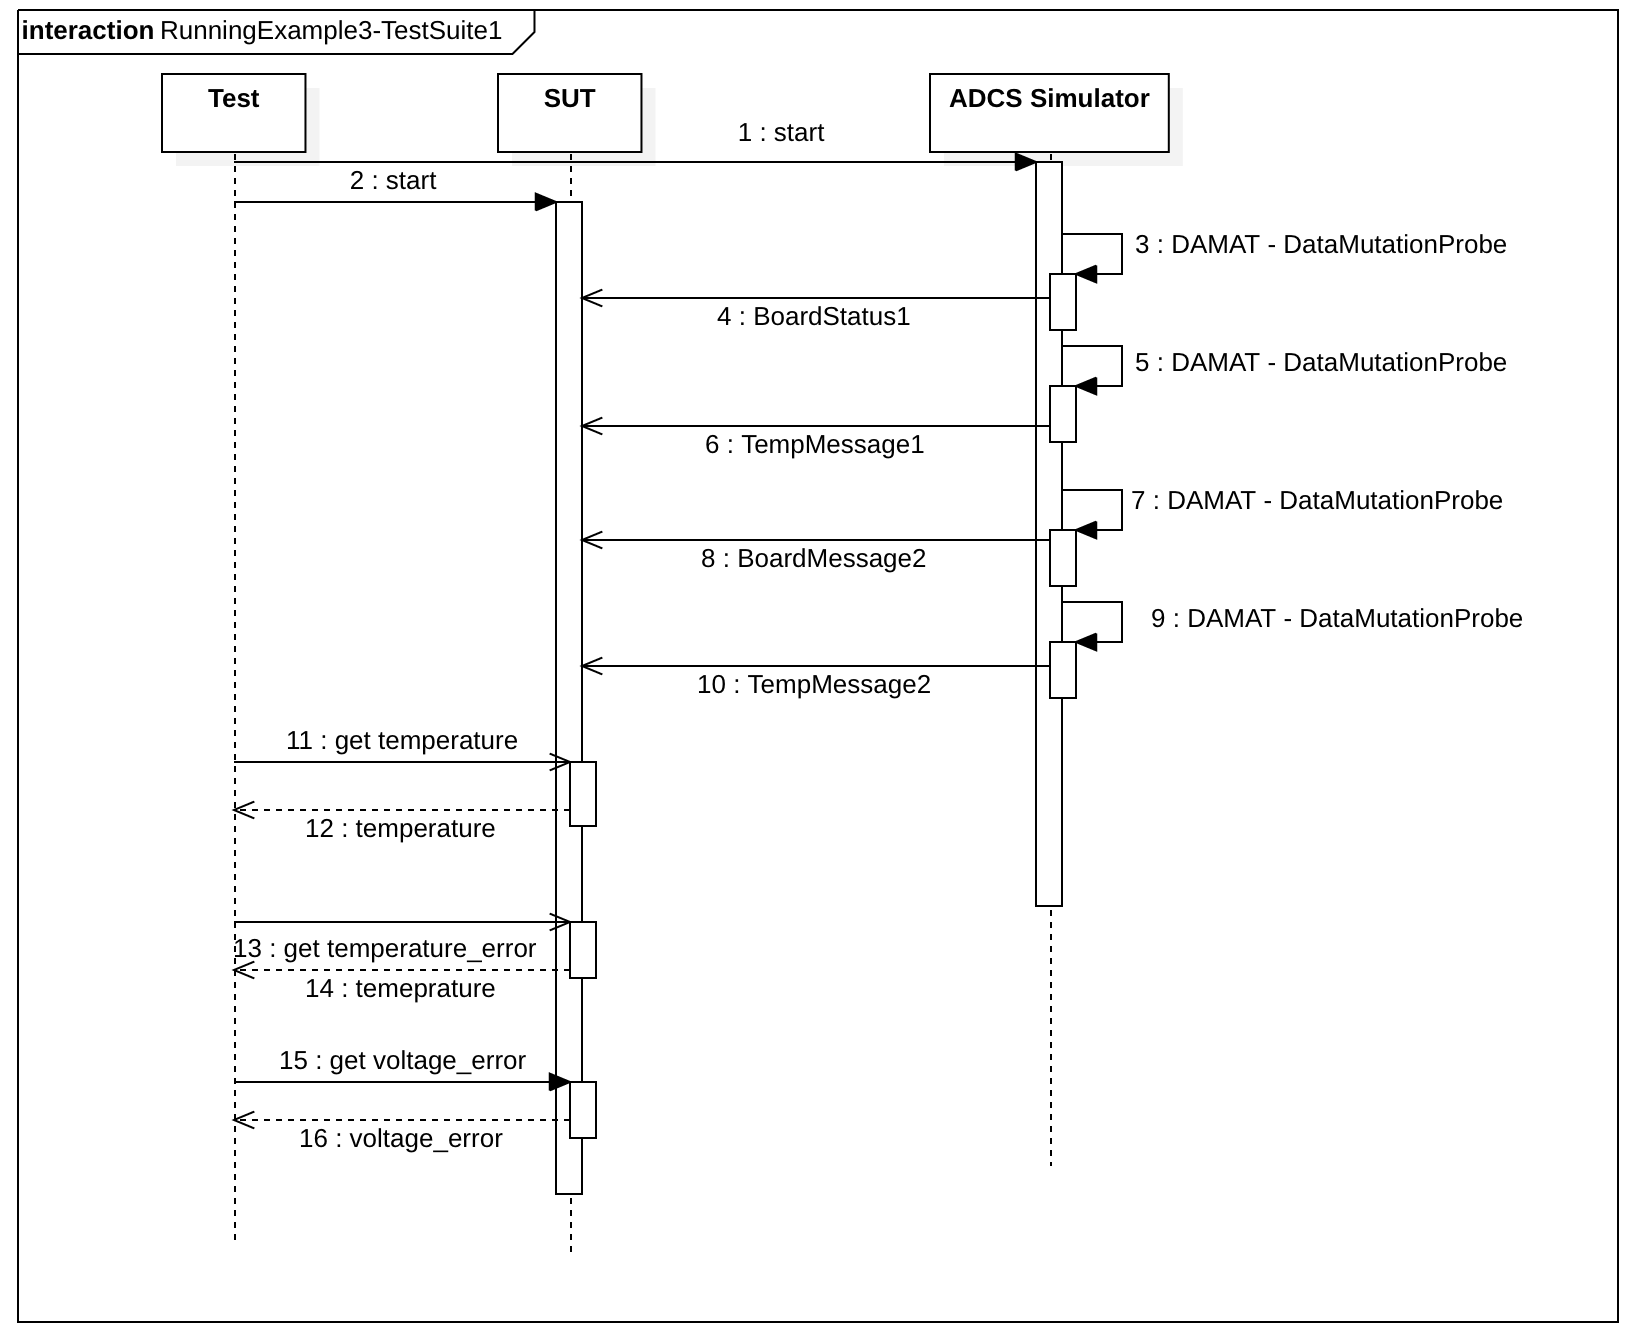
\includegraphics[width=8cm]{damat/images/RunningExampleSequence3.png}
\caption{Interactions exercised by the test cases of TestSuite1 in the running example set 3.}
\label{fig:damat:RunningExample3Sequence}
\end{figure}

Figures~\ref{fig:damat:RunningExample3A} and~\ref{fig:damat:RunningExample3B} show the data exchanged in our running example. With respect to the example set 1, the fault model includes also one VOR and FVOR operator to mutate the BoardStatus message. In Figures~\ref{fig:damat:RunningExample3A} and~\ref{fig:damat:RunningExample3B}, in the row named \emph{PASS}, we explicitly indicate the result of each test case (i.e., PASS or FAIL).

TestSuite1 covers all the possible combinations of values for the sequence of messages reporting about messages voltage error absent (true or false), temperature alarm absent (true or false), voltage error absent (true or false), temperature alarm absent (true or false); indeed, in total, we have 16 test cases.

TestSuite1 kills MUTANT 1. MUTANT 1 applies VAT, that is, it sets the temperature value above the threshold when it is below the threshold. To not kill MUTANT 1, the test suite should not include any failing oracle. Since the failing oracles include the complete set of oracles that either verify the temperature being in the nominal range or verify the absence of a temperature alarm, we conclude that whenever MUTANT 1 is not killed, we cannot be in the presence of an equivalent mutant but in the presence of a test suite limitation.

TestSuite1 kills MUTANT 2. MUTANT 2 applies FVAT, that is, it sets the temperature value below the threshold when it is above the threshold. To not kill MUTANT 2, the test suite shall not include any of the failing oracles. Since the failing oracles include the complete set of oracles that either verify the temperature being out of the nominal range or verify the presence of a temperature alarm, we conclude that whenever MUTANT 2 is not killed, we cannot be in the presence of an equivalent mutant but in the presence of a test suite limitation.

TestSuite1 kills MUTANT 3. MUTANT 3 applies the first mutation procedure of VOR, that is, it sets the value above range if it is within range. To not kill MUTANT 2, the test suite shall not include any of the failing oracles. Since the failing oracles include the complete set of oracles that either verify the temperature being in the nominal range or verify the absence of a temperature alarm, we conclude that whenever MUTANT 3 is not killed, we cannot be in the presence of an equivalent mutant but in the presence of a test suite limitation.

TestSuite1 kills MUTANT 4. MUTANT 4 applies the second mutation procedure of VOR, that is, it sets the value below range if it is in range. MUTANT 4 leads to the same system outputs as MUTANT 3 thus we can make the same conclusion (no equivalent mutant possible).

TestSuite1 kills MUTANT 5. MUTANT 5 applies the first mutation procedure of FVOR, that is, it sets the value within range if it is above range. 
To not kill MUTANT 5, the test suite shall not include any of the failing oracles. All the failing oracles belong to test cases that verify a scenario in which a voltage error is present just before the last temperature message is collected; consequently, the lack of such oracles would indicate a major limitation of the test suites (i.e., it would not test if the software identifies the error condition simulated by the scenario under test). Similarly, MUTANT 5 is killed if all such test cases would be missing; even in this case we would be in the presence of a major test suite limitation (i.e., the test suite does not simulate an important error condition). We thus conclude that MUTANT 5 cannot lead to equivalent mutants. 

TestSuite1 does not kill MUTANT 6. MUTANT 6 applies the second mutation procedure of FVOR, that is, it sets the value in range if it is below range. Since no values below range are observed during the execution of the test cases, \APPR never applies this mutation operation. For this reason the mutation operation for the test suite is 83\% (i.e., five out of six mutation operation are covered). Although TestSuite1 seems complete because it tests all the pairwise combinations of the conditions \emph{voltage error absent} and \emph{temperature alarm absent}, \APPR enables us to determine that when defining the test suite we did not consider the fact that the input partitions for voltage error are three (i.e., voltage within range, voltage above range, and voltage below range) not two (i.e., voltage error absent, voltage error present).




\begin{figure}[tb]
\centering
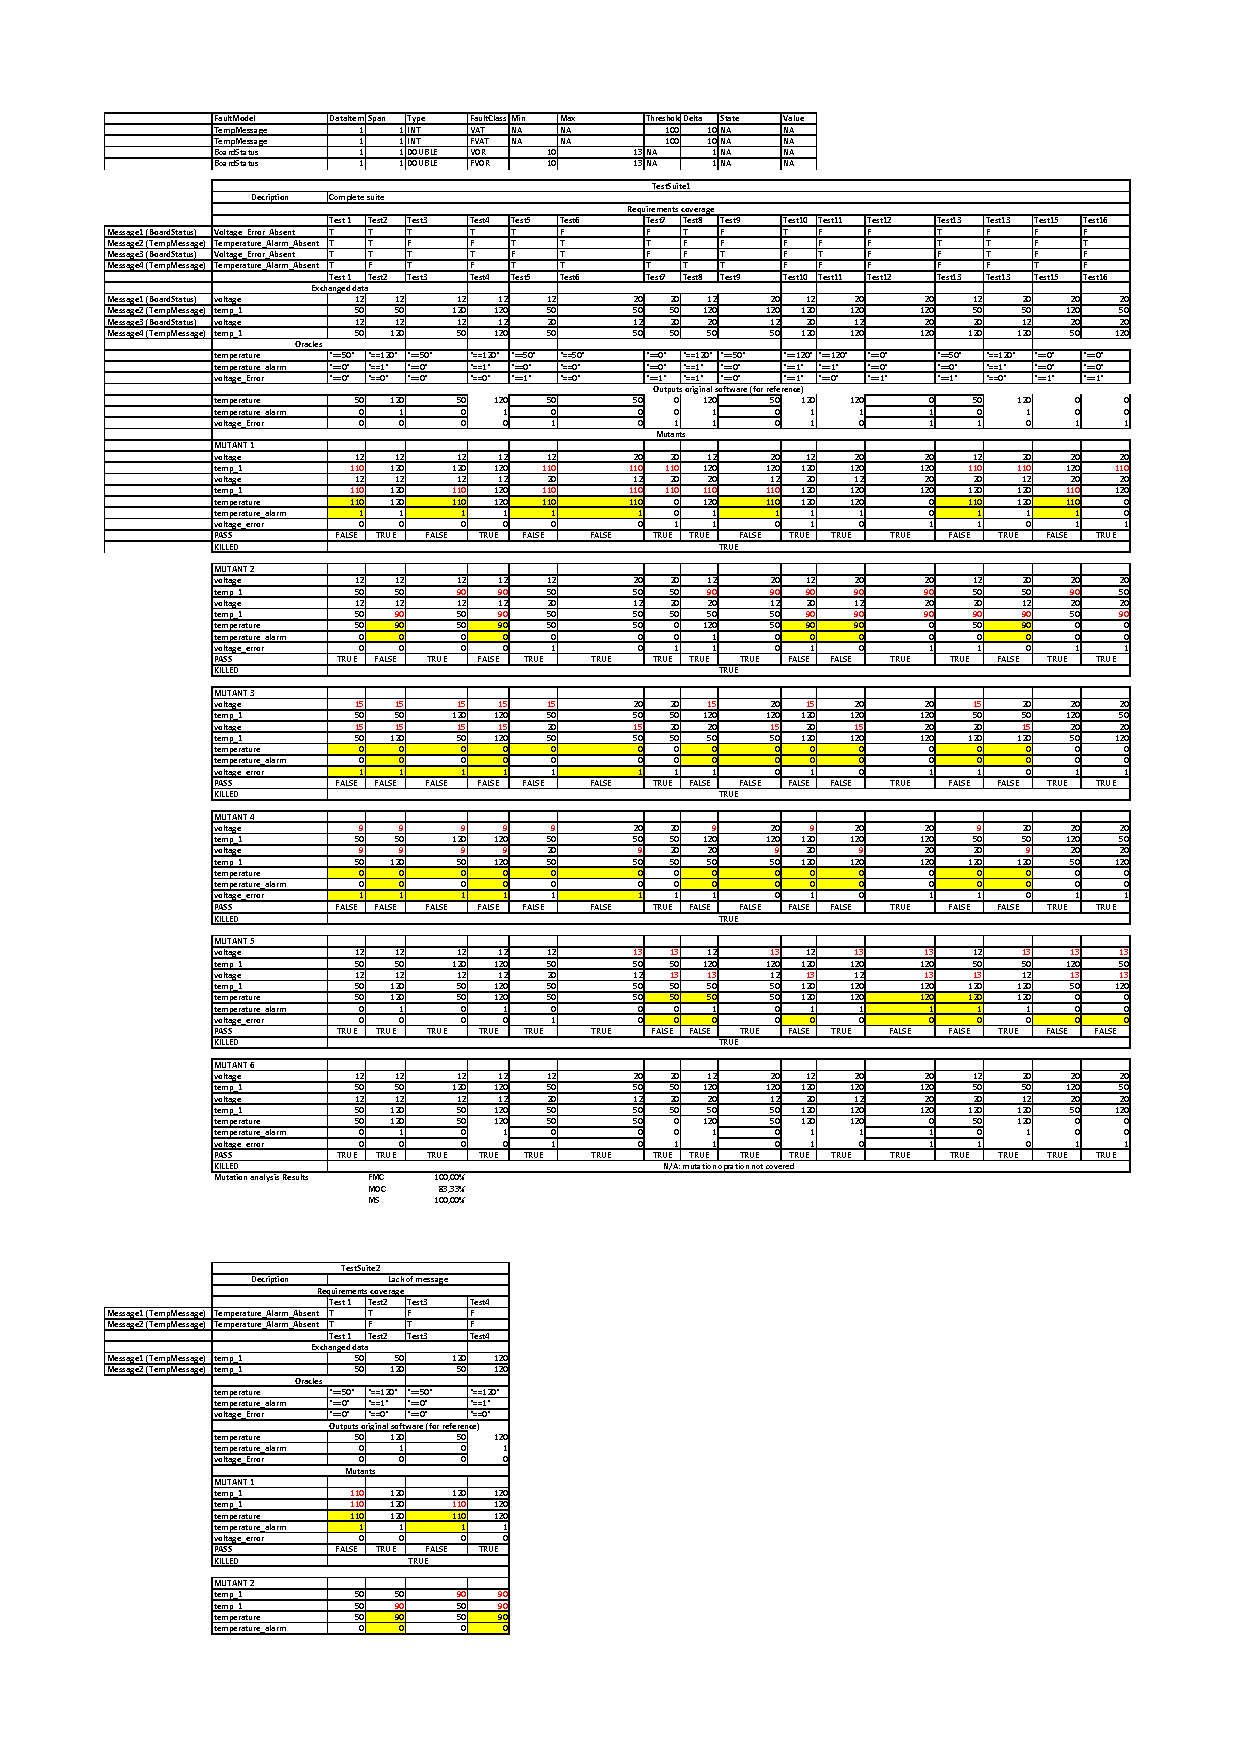
\includegraphics[width=18cm]{damat/DataDrivenExample3A}
\caption{Running example set 3 - Part A.}
\label{fig:damat:RunningExample3A}
\end{figure}

\begin{figure}[tb]
\centering
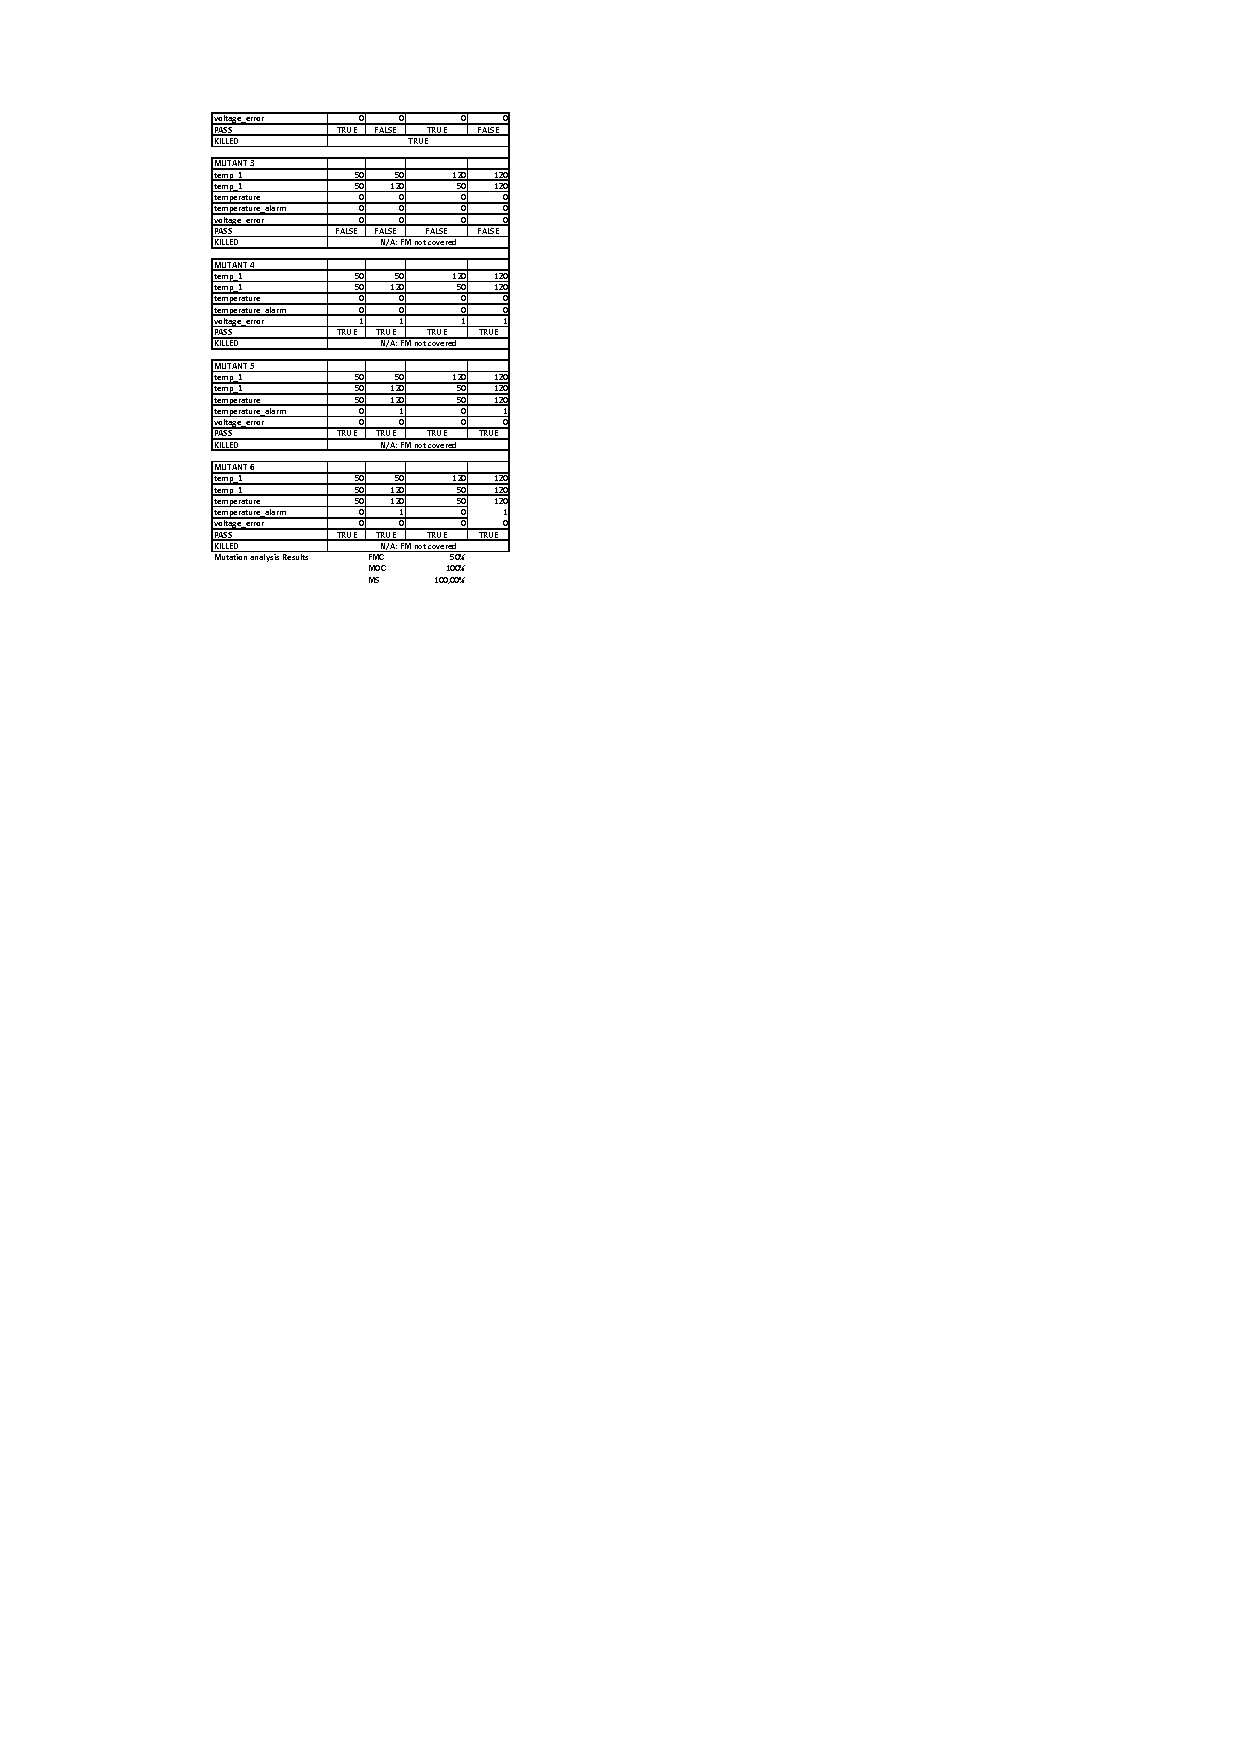
\includegraphics[width=18cm]{damat/DataDrivenExample3B}
\caption{Running example set 3 - Part B.}
\label{fig:damat:RunningExample3B}
\end{figure}


\paragraph{TestSuite2}



\begin{figure}[tb]
\centering
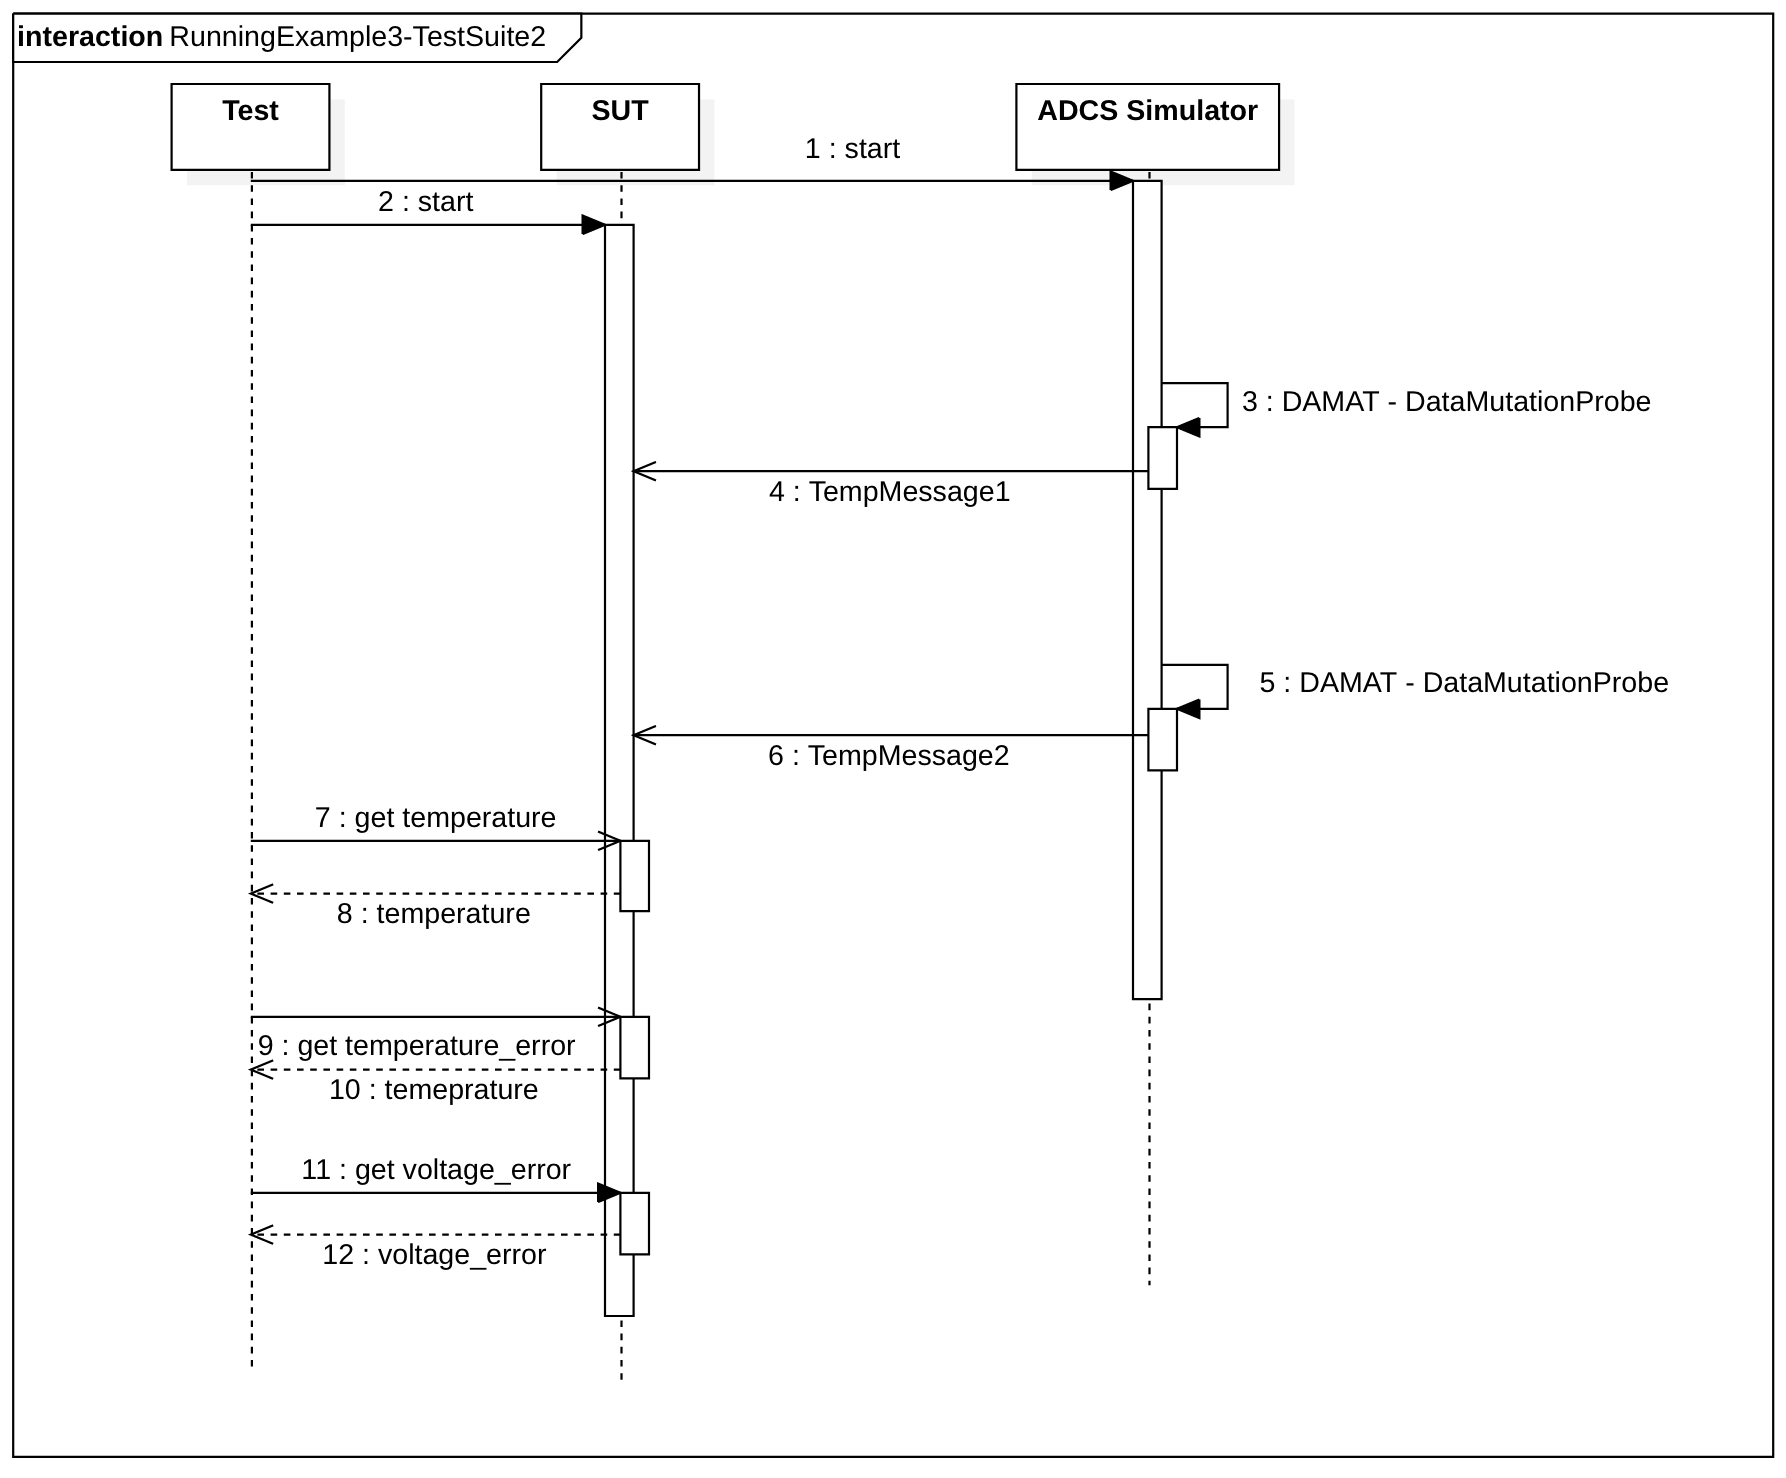
\includegraphics[width=8cm]{damat/images/runningExamplesSequence3_2.png}
\caption{Interactions exercised by the test cases of TestSuite2 in the running example set 3.}
\label{fig:damat:RunningExample3Sequence2}
\end{figure}

TestSuite 2 does not trigger messages of type BoardStatus; its interactions are depicted in Figure~\ref{fig:damat:RunningExample3Sequence2}. For the remaining message type (i.e., TempMessage) it covers all the possible combinations of temperature alarms being present/absent for two TempMessages sent in sequence; in total, we have 4 test cases.

The fault model BoardStatus is not covered; therefore the fault model coverage (FMC) is 50\%. Since MUTANTS 3 to 6 belong to BoardStatus they are not considered in the computation of the other mutation analysis metrics. MOC and MS are thus 100\%; indeed all the mutants not belonging to BoardStatus are killed by the test suite.

MUTANT 1 could be live only if relevant oracles are missing; more precisely, only if oracles concerning the nominal temperature value are missing. MUTANT 1 is killed by TestSuite2.

MUTANT 2 could be live only if relevant oracles are missing; indeed, only if oracles concerning the non nominal temperature value are missing. MUTANT 2 is killed by TestSuite2.
% !TEX root = MAIN.tex




\section{Data-driven Mutation Testing: DAMTE} % (fold)
\label{sec:data:test_suite_augmentation}



The \INDEX{test suite augmentation process} it consists of four activities \INDEX{Identify Test Inputs}, \INDEX{Generate Test Oracles}, \INDEX{Execute the SUT}, \INDEX{Fix the SUT}. It has the objective of increasing the score generated by the mutation analysis process.

FAQAS focussed on a methodology (i.e., data-driven mutation testing, \INDEX{DAMTE}) that specifies how to rely on KLEE to generate test inputs that increase the fault model coverage and the mutation operation coverage.
FAQAS does not address increasing the mutation score because infeasible in automated manner.
We recall that two might be the reasons for a low MS: poor oracle quality and missing test input sequences.
If the low mutation score is due to poor oracle quality, manual work is needed because automated approaches to automatically generate test oracles in the presence of system or integration test suites are not available. 
If the low mutation score is due to missing test input sequences (i.e., the software does not reach the state in which it could kill the mutant), manual work is required because existing test generation approaches (e.g., KLEE) might suffer from scalability problem that prevent bringing the system into a desired state; also, they cannot deal with systems whose components communicate through channels. 

For the cases targeted by FAQAS (i.e.,
in the presence of fault model coverage and mutation operation coverage below 100\%), test generation has the objective of generating test inputs that enable the application of all the mutation operators. 
We thus rely on an  \INDEX{extended data mutation probe} that
invokes a version of the data mutation API that instead of mutating the data targeted by the mutation operator not covered by the fault model, includes a reachability assertion that is used to make KLEE find a test input that reaches the mutant code. The test input shall then be inspected by the engineer, who will need then to integrate it into his test suite.
%Figure~\ref{fig:dataDrivenTestSuiteAugmentationB} exemplifies how data driven mutation testing works, for the producer consumer and client-server cases.
%
%
%
%
%\begin{figure}[h]
%  \centering
%    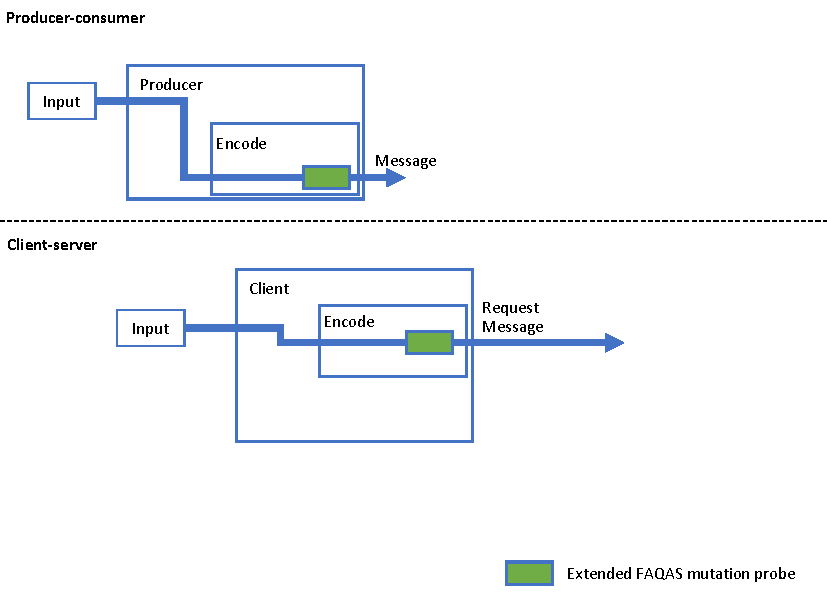
\includegraphics[width=14cm]{images/dataDrivenTestSuiteAugmentationB}
%      \caption{Data-driven mutation analysis for different architectures.}
%      \label{fig:dataDrivenTestSuiteAugmentationB}
%\end{figure}










%%
%% The acknowledgments section is defined using the "acks" environment
%% (and NOT an unnumbered section). This ensures the proper
%% identification of the section in the article metadata, and the
%% consistent spelling of the heading.
%\begin{acks}
%Acks
%\end{acks}

%%
%% The next two lines define the bibliography style to be used, and
%% the bibliography file.
\bibliographystyle{ACM-Reference-Format}
\bibliography{./bibliography.bib}



\end{document}
\endinput
%%
%% End of file `sample-authordraft.tex'.
